%%
% BIThesis 本科毕业设计论文模板（全英文） —— 使用 XeLaTeX 编译 The BIThesis Template for Undergraduate Thesis
% This file has no copyright assigned and is placed in the Public Domain.
% Compile with: xelatex -> biber -> xelatex -> xelatex
%%

% !TeX program = xelatex
% !BIB program = biber

% 我校英文论文尚无统一规范，目前存在各种学院变体，请参考 README.md 调整。

% 开启盲审格式 blindPeerReview=true (如：[type=bachelor_english,blindPeerReview=true])

\documentclass[type=bachelor_english]{bithesis}

% 若需中文封面或在经管学院，请参考 ./README.md 中「BITSetup 学院变体」一节。
% 此处仅列出常用的配置。全部配置用法请见「bithesis.pdf」手册。
\BITSetup{
  cover = {
    % 封面需要「北京理工大学」字样图片，如无必要请勿修改该项。
    headerImage = images/header.pdf,
    % 封面标题需要“华文细黑”，如无必要请勿修改该项。
    xiheiFont = STXIHEI.TTF,
    % 可用以下参数自定义封面日期。
    % date = {November 5, 1955},
  },
  info = {
    % 想要删除某项封面信息，直接删除该项即可。
    % 想要让某项封面信息留空（但是保留下划线），请传入空白符组成的字符串，如"{~}"。
    % 如需要换行，则用 “\\” 符号分割。
    title = 基于多模态数据的目标融合与行为分析系统设计,
    titleEn = {Design of a Target Fusion and Behavior Analysis System Based on Multimodal Data},
    school = School of Computer,
    major = Computer Science and Technology,
    author = Wang Chenxu,
    studentId = 1120223433,
    supervisor = Pang Jinhui,
    keywords = {多模态目标融合；视觉地点识别；时空图建模；图匹配；行为异常检测},
    keywordsEn = {Multimodal Target Fusion; Visual Place Recognition; Spatiotemporal Graph Modeling; Graph Matching; Behavior Anomaly Detection},
    % 如果你的毕设为校外毕设，请将下面这一行语句解除注释（删除第一个百分号字符）并填写你的校外毕设导师名字
    externalSupervisor = Zhang Haitao,
  },
  % 有些专业名带上“Bachelor of…”太长，学院可能建议把 degree 改成 major。
  % 若要将封面的“Degree:”改为“Major:”，请解除下一行的注释。
  % const/info/major = {Major},
  %
  style = {
    % 页眉若要改为中文，请解除下一行的注释。
    % head = {北京理工大学本科生毕业设计（论文）},
    %
    % 开启该选项后，将用 Times New Roman 的开源字体 TeX Gyre Termes 作为正文字体。
    % 这个选项适用于以下情况：
    % 1. 不想在系统中安装 Times New Roman。
    % 2. 在 Linux/macOS 下遇到 `\textsc` 无法正常显示的问题。
    betterTimesNewRoman = true,
  },
  misc = {
    % 微调表格行间距
    tabularRowSeparation = 1.25,
  },
}

% 这份模板提供了代码块示例，采用 listings 宏包及其预定义样式。
% 使用代码块时，也可选用自己的喜欢的其他宏包，如 minted：https://bithesis.bitnp.net/faq/minted.html
% 如果不需要，直接删除即可。
\usepackage{listings}
\usepackage{float}
\usepackage{pdflscape}


% 大部分关于参考文献样式的修改，都可以通过此处的选项进行配置。
% 详情请搜索「biblatex-gb7714-2015 文档」进行阅读。
\usepackage[
  backend=biber,
  style=gb7714-2015,
  gbalign=gb7714-2015,
  gbnamefmt=lowercase,
  gbpub=false,
  doi=false,
  url=false,
  eprint=false,
  isbn=false,
]{biblatex}

% 参考文献引用文件位于 misc/ref.bib
\addbibresource{misc/ref.bib}

% 若要按计算机学院要求，添加“北京理工大学”水印，请参考
% https://bithesis.bitnp.net/faq/watermark.html

% 文档开始
\begin{document}

% 标题页面：如无特殊需要，本部分无需改动
\MakeCover

% 原创性声明：盲审结束前无需改动
\MakeOriginality
% 后续添加签名时，可考虑先用 Word 制作再导出到 misc/0_originality.pdf，
% 同时注释以上 `\MakeOriginality`，解除注释以下三行代码。
% \begin{blindPeerReview}
%   \includepdf{misc/0_originality.pdf}\newpage
% \end{blindPeerReview}

% 前置内容定义
\frontmatter
% 摘要：在相应 TeX 文件撰写
\begin{abstract}
本文围绕基于多模态数据的目标融合与行为分析系统设计展开研究。针对复杂场景中单一观测手段信息不完整、目标身份难以保持一致以及群体行为理解不足等问题，本文综合利用光学图像、电磁观测数据、合成孔径雷达图像及相关轨迹信息，构建从目标轨迹接入、跨模态目标融合到行为异常分析的完整技术流程，以提高复杂环境下目标表征、目标关联和态势理解的可靠性。
系统框架主要包括四个部分。首先，针对缺少地理坐标的光学图像，引入基于视觉地点识别的参考图像检索方法，并结合后续跨图像目标关联，使图像平面中的目标观测能够接入已有轨迹体系。其次，面向多源观测中存在的缺失、异步和噪声问题，建立统一的数据表示与时空图建模方式，为后续跨模态处理提供结构化输入。再次，构建基于轨迹编码和多集合图匹配的多模态目标融合方法，通过实体级配准实现不同观测源之间的目标对应和信息融合。最后，在融合后的目标轨迹基础上进行个体行为和群体行为分析，利用异常检测、群体时空一致性建模和态势热力图生成等方法输出可解释的行为分析结果。
实验与分析表明，所设计的各功能模块能够分别支持无坐标光学图像的参考检索、多模态目标实体配准以及基于融合轨迹的行为异常分析。本文的研究为复杂场景下多源目标数据的统一组织、可靠融合和高层行为理解提供了一种系统化实现思路。
项目代码、实验脚本、可视化材料和论文相关文件已公开于：\url{https://github.com/wcx12/FusionTrack}。
\end{abstract}

\begin{abstractEn}
This thesis studies the design of a target fusion and behavior analysis system based on multimodal data. The research focuses on integrating optical imagery, electromagnetic observation data, SAR imagery, and related trajectory information to improve target representation, target association, and group behavior understanding in complex scenes.
The overall framework consists of four major stages. First, for optical images without geographic coordinates, a reference image retrieval and trajectory access procedure is designed based on visual place recognition and cross-image target association, so that pixel-level target observations can be connected to the existing trajectory system. Second, unified data representation and spatiotemporal graph modeling are introduced to handle missing, asynchronous, and noisy multimodal observations. Third, a multimodal target fusion method is constructed through trajectory encoding and multi-set graph matching, enabling entity-level registration and fusion across heterogeneous sources. Fourth, behavior analysis is performed on the fused target data through individual anomaly detection, group spatiotemporal consistency modeling, and situation heatmap generation.
The experiments and analyses show that the proposed modules can support reference retrieval for coordinate-missing optical images, entity-level multimodal target registration, and behavior anomaly analysis based on fused trajectories. This thesis provides a systematic implementation route for organizing, fusing, and interpreting multisource target data in complex scenes.
The project code, experimental scripts, visualization materials, and thesis-related files are publicly available at: \url{https://github.com/wcx12/FusionTrack}.
\end{abstractEn}


\MakeTOC

% 正文开始
\mainmatter

% 在这里引用各章 TeX 文件，按需添加
\chapter{Introduction}

\section{Research Background and Significance}
Reliable target understanding in complex dynamic scenes requires more than object detection in individual frames. A practical perception system must estimate where a target is, how it moves, whether it corresponds to an existing entity, and whether its behavior departs from normal scene evolution. These requirements are central to situation awareness, where low-level observations are converted into target states and higher-level scene interpretation \cite{endsley1995situation,blasch2009blueprint}. Target fusion and behavior analysis are therefore coupled tasks: behavior analysis depends on target states that are complete, consistent, and interpretable.

Single-modal sensing rarely satisfies these requirements in realistic environments. Optical images provide rich appearance, category, and contextual information, but they are sensitive to illumination, viewpoint, occlusion, weather, and missing geographic metadata. Electromagnetic and radar-like observations can provide complementary physical or motion-related cues, although they often carry weaker semantic information. Synthetic aperture radar (SAR) supports wide-area and all-weather observation, yet its imaging mechanism differs substantially from optical sensing. Existing trajectory records add temporal continuity and historical context, but they may be incomplete or inconsistent with newly observed targets. These complementary strengths motivate multimodal fusion rather than reliance on any single source.

Multimodal data become useful only after their cross-source relationships are made explicit. Different sensors may use different coordinate systems, sampling rates, spatial resolutions, and uncertainty models. They may also assign different identifiers to the same physical target. In some optical images, geographic coordinates may be unavailable. Target detections from these images then remain in the image plane and cannot directly enter a georeferenced trajectory system. If such observations are fused without reliable spatial and identity relationships, the resulting target states may contain false associations.

These limitations motivate the processing chain studied in this thesis. Coordinate-missing optical images are first connected to the trajectory system through visual reference retrieval and downstream target association. The resulting optical observations are then aligned with heterogeneous target entities through graph-based registration. The fused trajectories finally support individual and group behavior analysis. This design treats optical access, cross-modal fusion, and behavior analysis as connected stages rather than separate tasks. The following section formalizes this connected problem.

\section{Problem Description}
This thesis considers multimodal target fusion and behavior analysis under heterogeneous and partially incomplete observations. The available data include optical images with or without geographic metadata, target detections or modality-specific track fragments, electromagnetic observations, SAR observations, and existing target trajectories. These data sources provide complementary information, but they are not directly comparable. They may differ in spatial reference, temporal coverage, feature representation, and target identity assignment. The objective is to transform these heterogeneous observations into consistent entity-level target trajectories and then use the fused trajectories for behavior anomaly analysis and situation presentation.

A key sub-problem is the access of coordinate-missing optical images to the existing trajectory system. For coordinate-known optical images, detected targets can be represented in a common spatial frame and then considered by downstream target-association methods. For coordinate-missing optical images, however, target detections remain in the image plane and cannot be directly compared with georeferenced trajectories. Therefore, this thesis treats optical reference retrieval as a prerequisite for optical trajectory access. The retrieval result provides coordinate-known reference candidates and constrains the downstream target-level association process. It does not directly determine target identity or recover complete geographic trajectories.

Another sub-problem is entity-level registration across modalities. After single-modal preprocessing, each modality may produce its own target observations or trajectory fragments. These modality-specific target sets may contain the same physical targets, but their attributes, noise levels, sampling times, and confidence values can differ. The fusion problem is therefore not only to combine features, but also to estimate which entities from different modalities correspond to the same target. This thesis formulates the task as cross-modal entity registration, where target representations and relational structures are jointly used to estimate correspondences.

The final sub-problem is behavior analysis based on fused target trajectories. The fused trajectory is regarded as the target-level representation for subsequent analysis. Individual anomalies may appear as route deviation, abnormal speed, unusual trajectory shape, or sudden state change. Group-level anomalies may appear as inconsistent local motion, target departure from a group, group splitting, or group merging. The behavior analysis task is therefore defined as estimating interpretable anomaly indicators from both individual trajectories and group spatiotemporal relations.

Overall, the thesis addresses a connected problem chain. Coordinate-missing optical observations are first connected to the trajectory system through reference retrieval and target-level association constraints. Heterogeneous target entities are then aligned and fused. The fused trajectories are finally used for behavior analysis. This formulation separates the problem definition from the detailed technical challenges and provides the basis for the following chapters.

\section{Key Challenges}
The problem formulation above leads to several technical challenges. These challenges arise not only from the heterogeneity of the data sources, but also from the uncertainty that propagates across optical access, multimodal fusion, and behavior analysis.

Visual reference uncertainty is introduced by missing spatial metadata. Coordinate-missing optical images do not directly provide target locations in the same frame as existing trajectories. Their visual content may contain useful scene cues, but those cues can be distorted by viewpoint changes, illumination variation, seasonal appearance changes, occlusion, and dynamic objects. As illustrated in Fig.~\ref{fig:intro-vpr-challenges}, the same place may present different visual appearances across observation conditions. Training-based VPR also introduces an additional deployment burden because new scenes may lack labeled image pairs for training or domain adaptation. As a result, the system must establish reliable visual reference relationships under limited supervision and large appearance variation.

\begin{figure}[htbp]
  \centering
  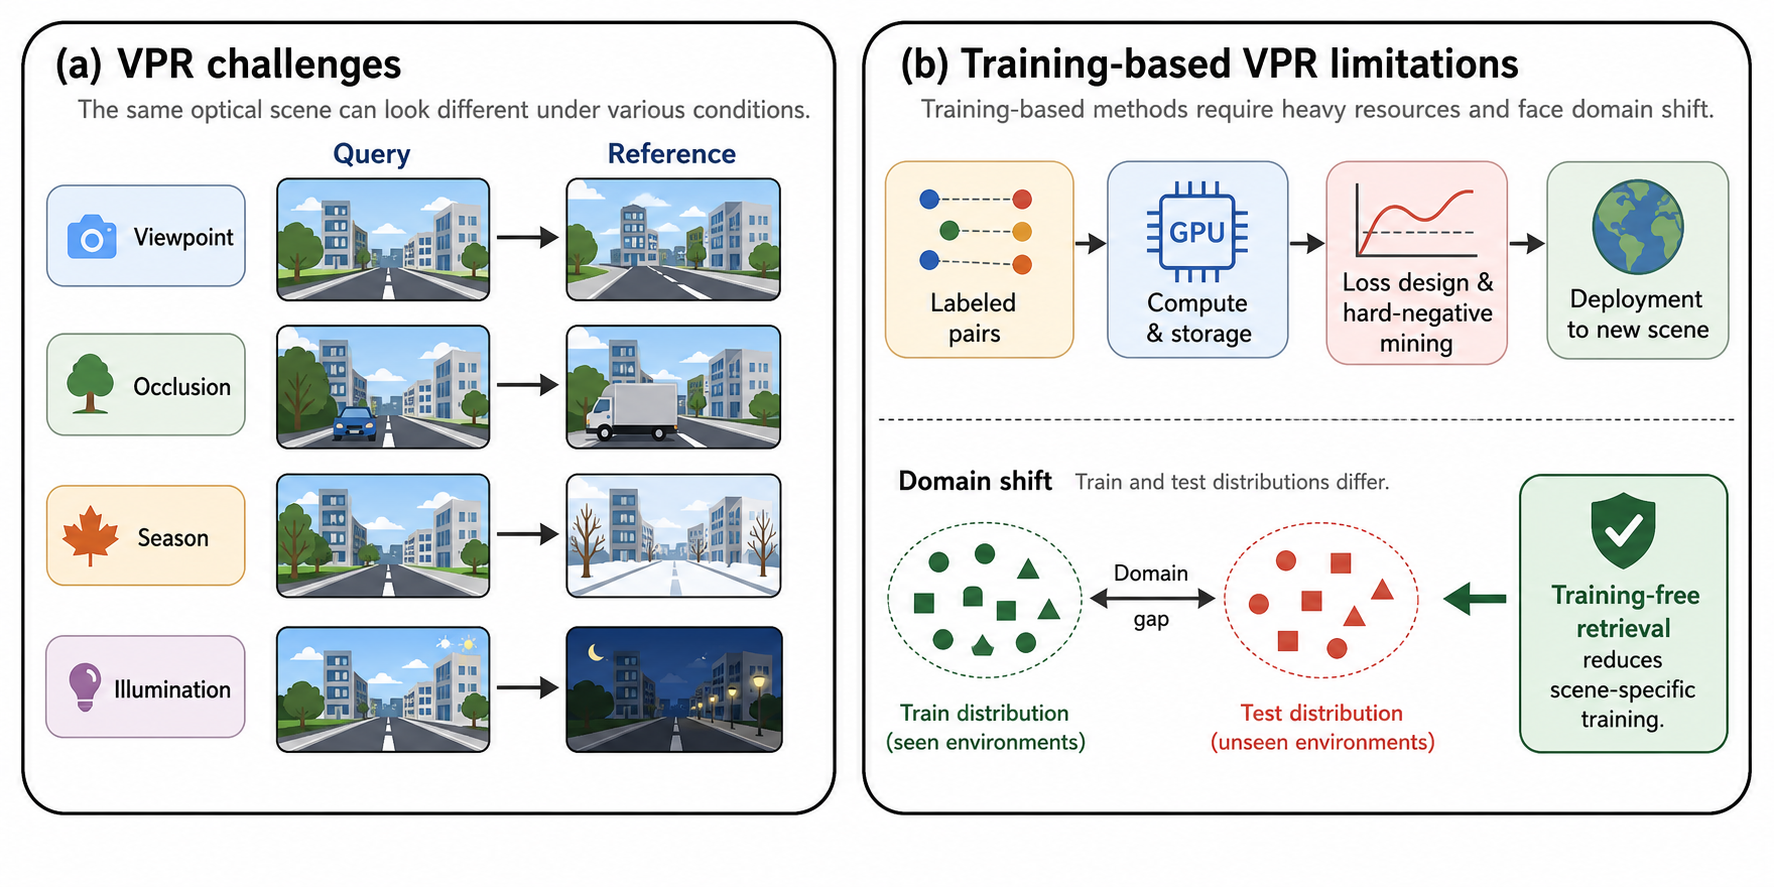
\includegraphics[width=0.95\linewidth]{images/chapter1/vpr_challenges_training_free_motivation.png}
  \caption{Conceptual illustration of VPR challenges and training-based VPR limitations in coordinate-missing optical scenes.}
  \label{fig:intro-vpr-challenges}
\end{figure}

Multimodal observation also introduces temporal inconsistency and incompleteness. This challenge is summarized in Fig.~\ref{fig:intro-temporal-inconsistency}, where optical, electromagnetic, and SAR observations are shown as separate timelines rather than naturally aligned frames. The colored windows indicate intervals in which a modality can provide observations, while the markers and gray crosses distinguish valid observations from missing ones at the reference times. The figure therefore makes two sources of incompleteness explicit. First, temporal incompleteness arises because sensors have different sampling rates and may produce interrupted tracklets. Second, spatial incompleteness arises because the sensor footprints or fields of view may not cover the same region at the same time. As a result, a target can be observed in one modality while absent in another, and a reference time may contain only partial or asynchronous evidence. Direct frame-level fusion is unstable under this condition because a complete synchronized multimodal observation tuple cannot be assumed. The fusion representation must instead tolerate missing observations, align asynchronous tracklets, and account for modality-dependent reliability.

\begin{figure}[H]
  \centering
  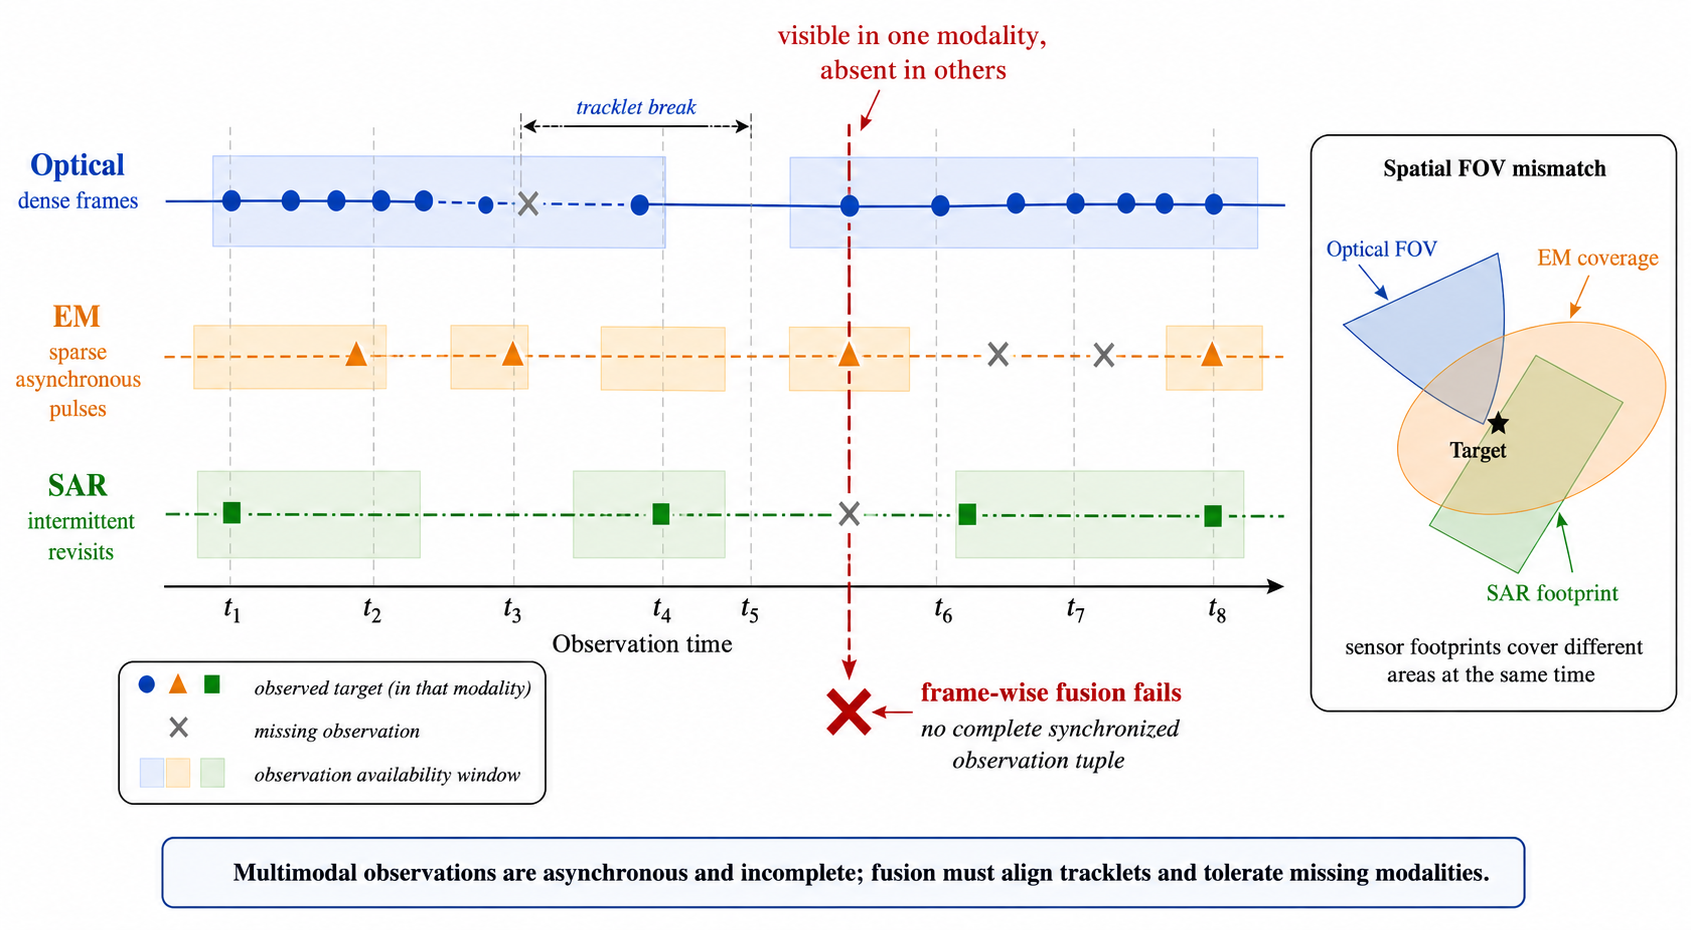
\includegraphics[width=0.95\linewidth]{images/chapter1/temporal_inconsistency_incomplete_observation.png}
  \caption{Temporal inconsistency and incompleteness in multimodal observation. The figure shows why asynchronous sampling, interrupted observations, and spatial coverage mismatch make direct frame-level fusion unreliable.}
  \label{fig:intro-temporal-inconsistency}
\end{figure}

Cross-modal identity ambiguity further arises from heterogeneous representations. As illustrated in Fig.~\ref{fig:intro-cross-modal-identity}, each modality may form its own target graph with modality-specific node attributes, missing entities, and neighborhood relations. Optical observations mainly provide appearance and semantic cues, electromagnetic observations describe signal-related responses, and SAR observations capture scattering and spatial response patterns. These heterogeneous representations create two coupled difficulties. First, different targets within one modality may have similar local features, such as visually similar optical targets. Second, the same physical target may appear dissimilar across modalities because its optical appearance, electromagnetic signal, and SAR response are generated by different sensing mechanisms. The local similarity matrices in Fig.~\ref{fig:intro-cross-modal-identity} show the resulting ambiguity: a feature-only matcher may produce multiple high-score candidate correspondences, such as several optical targets competing for one electromagnetic target or one electromagnetic target being compatible with multiple SAR detections. Therefore, cross-modal association cannot rely only on local feature similarity. It must be treated as a graph-level assignment problem that jointly exploits temporal continuity, spatial compatibility, and relational structure among targets.

\begin{figure}[H]
  \centering
  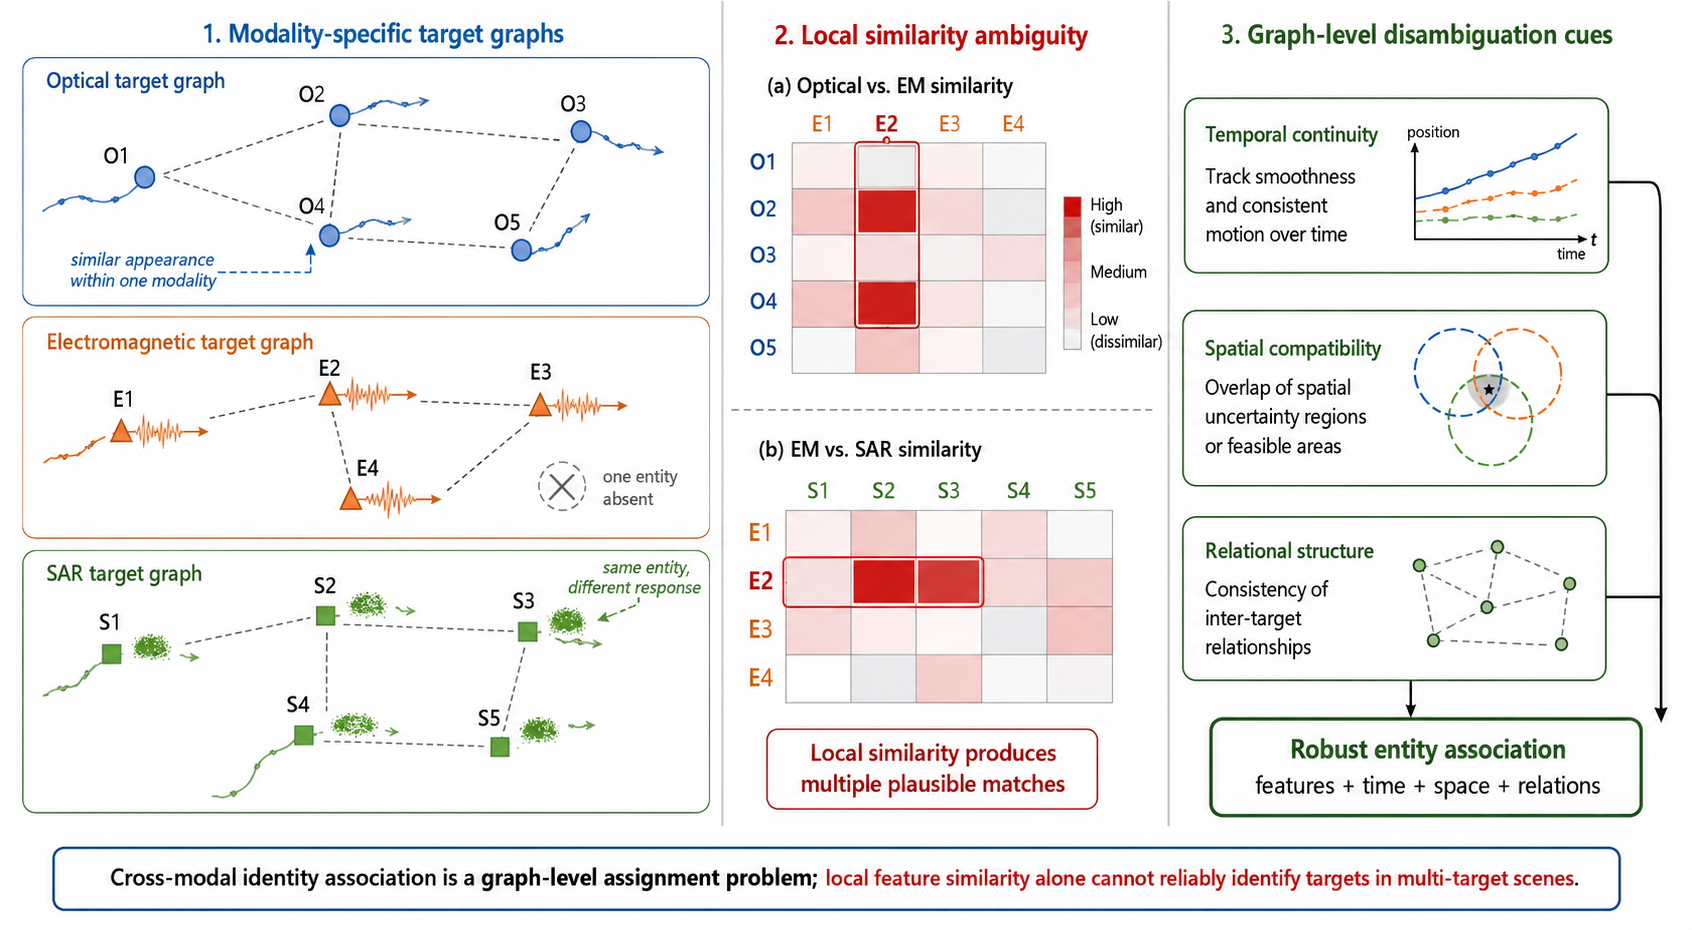
\includegraphics[width=0.98\linewidth]{images/chapter1/cross_modal_identity_ambiguity.png}
  \caption{Cross-modal identity ambiguity under heterogeneous target representations. The figure shows that local feature similarity can produce multiple plausible matches, so identity association must also use temporal, spatial, and relational consistency.}
  \label{fig:intro-cross-modal-identity}
\end{figure}

Behavior analysis must remain interpretable under fused-data uncertainty. As shown in Fig.~\ref{fig:intro-behavior-uncertainty}, the behavior analysis stage receives fused trajectories rather than ground-truth motion traces. These trajectories may still contain localization uncertainty, missing observations, cross-modal association errors, and noisy fused states caused by the previous optical access and multimodal fusion stages. The middle part of the figure separates behavioral evidence into two levels. Individual-level evidence describes route deviation, abnormal speed, and unusual motion shape, while group-level evidence describes relative motion changes, neighborhood structure variation, and membership changes. These two levels do not always agree. A trajectory may look normal in isolation but abnormal relative to its group. Conversely, a short individual anomaly may not indicate a meaningful situation-level event if the group relation remains stable. Therefore, the output should not be limited to a single anomaly score. It should combine uncertainty-aware score curves, explanation tags, and spatial event summaries so that the system can indicate both what is abnormal and how reliable the supporting evidence is. The behavior analysis method must therefore provide anomaly indicators that are robust to upstream uncertainty and interpretable for situation assessment.

\begin{figure}[H]
  \centering
  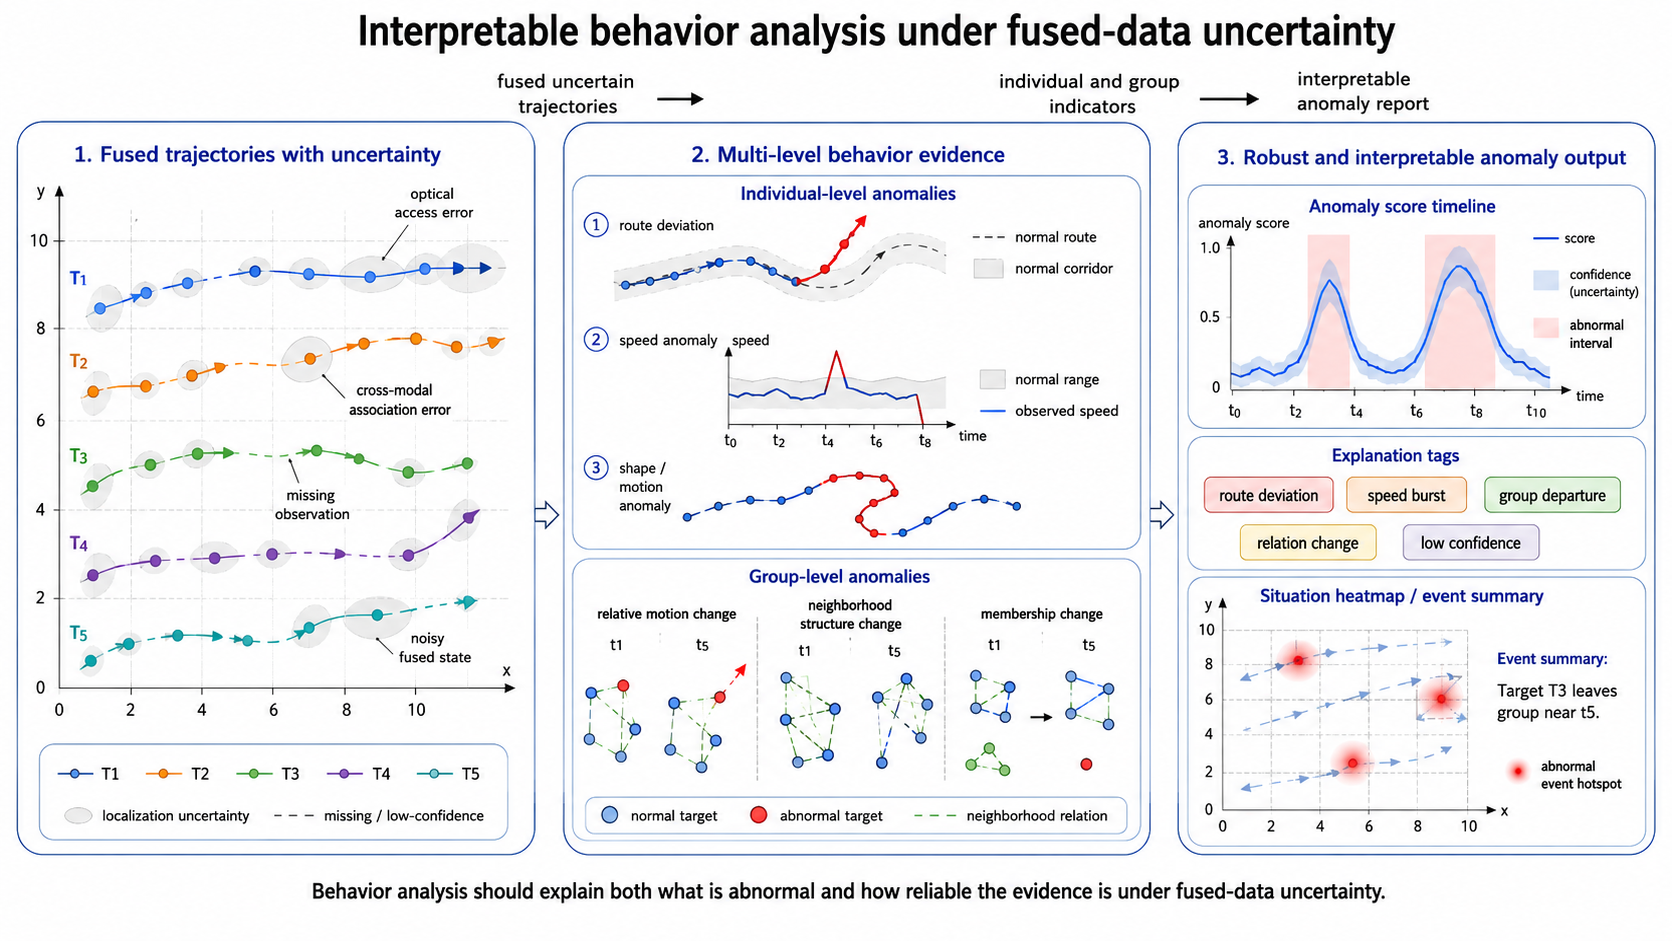
\includegraphics[width=0.98\linewidth]{images/chapter1/interpretable_behavior_uncertainty.png}
  \caption{Interpretable behavior analysis under fused-data uncertainty. The figure links uncertain fused trajectories to individual and group anomaly evidence, highlighting that the output should explain both abnormal behavior and evidence reliability.}
  \label{fig:intro-behavior-uncertainty}
\end{figure}

These challenges motivate a review of related work on visual place recognition, multimodal target fusion, graph-based registration, and trajectory-based anomaly detection.

\section{Related Work}

\subsection{Visual Place Recognition and Optical Trajectory Association}
Visual place recognition (VPR) aims to retrieve reference images that depict the same or a nearby physical location as a query image \cite{yin2025gprs,wang2026tfvpr}. It is a core component in robotic localization, loop-closure detection, long-term navigation, and visual retrieval \cite{murartal2017orbslam2,milford2008seqslam}. In this thesis, VPR is introduced for a narrower purpose. It supports coordinate-missing optical access by providing scene-level reference candidates, rather than by making target-level identity decisions.

The main difficulty in VPR is appearance variation. The same place may differ substantially across viewpoints, illumination conditions, seasons, occlusions, and domains \cite{yin2025gprs,wang2026tfvpr}. As shown in Fig.~\ref{fig:intro-vpr-challenges}, this difficulty is especially relevant to coordinate-missing optical images, because visual content is the only available cue for establishing a reference relationship with coordinate-known scenes.

Existing VPR methods have developed from hand-crafted retrieval pipelines to learned visual descriptors. Early systems often used local feature aggregation strategies such as Bag-of-Words and VLAD \cite{galvez2012bags,jegou2010vlad}. Deep VPR methods then improved descriptor discriminability through several complementary routes, including trainable VLAD-like aggregation, local-to-global patch matching, geographically structured supervision, viewpoint-robust training, and holistic feature mixing \cite{arandjelovic2016netvlad,hausler2021patchnetvlad,berton2022cosplace,berton2023eigenplaces,alibey2023mixvpr}. Graph-based VPR methods further exploit relationships among regions or patches to improve robustness under viewpoint changes and local ambiguity \cite{qin2021gatvpr,zuo2025prgs,chen2025sage}.

Despite these advances, many high-performing VPR methods still depend on scene-level supervision signals, such as paired place images, geographic labels, task-specific training objectives, or target-domain optimization \cite{arandjelovic2016netvlad,berton2022cosplace,alibey2023mixvpr}. These requirements limit their use when a new scene lacks reliable annotations. Large-scale visual pretraining provides a more flexible alternative: contrastive image-text learning, vision transformers, masked image modeling, and self-supervised dense representation learning have all shown the ability to produce transferable visual features \cite{radford2021clip,dosovitskiy2020vit,he2022mae,oquab2023dinov2}. AnyLoc shows that frozen foundation-model features can support zero-shot place recognition \cite{keetha2024anyloc}, while TF-VPR further studies training-free descriptor generation and refinement for VPR \cite{wang2026tfvpr}. This training-free direction matches the setting of this thesis. It reduces dependence on scene-specific annotation and provides coordinate-known reference candidates for downstream optical trajectory association. The detailed method is presented in Chapter 3.

\subsection{Multimodal Target Fusion}
Multimodal target fusion seeks to combine heterogeneous observations into target states that are more complete and reliable than those from a single sensor. Multisensor fusion research commonly distinguishes signal-level fusion, object-level estimation, and situation-level interpretation \cite{hall1997multisensor,blasch2009blueprint}. In target analysis, this hierarchy is often reflected in feature-level, decision-level, and target-level fusion.

Feature-level fusion projects heterogeneous observations into a shared representation before prediction or association. It can exploit complementary information at an early stage, but it usually assumes accurate temporal and spatial alignment. Decision-level fusion combines outputs from modality-specific models. This strategy is easier to deploy when sensors have separate processing pipelines, but it may lose fine-grained target interactions. Target-level fusion focuses on whether observations correspond to the same physical entity and how their states should be integrated. This level is most relevant to this thesis because behavior analysis requires consistent trajectories, not independent modality-specific decisions.

The central limitation of practical target-level fusion is that heterogeneous observations are rarely aligned in advance. Different modalities may have different sampling rates, localization accuracy, attribute spaces, and missing-observation patterns. Recent studies on multimodal registration and fusion show that cross-source alignment must account for geometry, semantics, uncertainty, and modality-specific reliability \cite{wu2024jointsemantic,chen2026multimodal,zhang2025optsar}. These requirements connect multimodal fusion to entity correspondence estimation. Graph modeling and registration therefore provide a more specific technical route for the present work.

\subsection{Graph Modeling and Entity-Level Registration}
Graph modeling provides a structured way to represent targets and their relations. A graph can encode target attributes as node features and describe temporal continuity, spatial neighborhoods, or contextual dependencies as edges. This representation is useful in multi-target scenes because identity consistency often depends on both local target evidence and relational structure.

Single-modal tracking methods provide an important basis for target identity maintenance. Classical probabilistic methods, including multiple hypothesis tracking and joint probabilistic data association, model uncertainty under missed detections and clutter \cite{reid1979mht,fortmann1983jpda}. Modern tracking-by-detection methods maintain trajectory continuity by combining efficient motion prediction, deep appearance association, low-confidence detection recovery, and robust association strategies such as camera-motion compensation \cite{bewley2016sort,wojke2017deepsort,zhang2022bytetrack,aharon2022botsort}. These methods are effective for producing modality-specific trajectories. However, they do not by themselves resolve correspondence between entities observed by different modalities.

Graph matching and registration extend this idea from within-modality association to cross-set alignment. Instead of matching isolated nodes independently, graph matching seeks correspondences supported by both node similarity and structural consistency. This property is valuable when local target features are ambiguous but relational roles remain informative. Registration methods have developed from iterative closest point and its variants \cite{besl1992icp,rusinkiewicz2001icpvariants,segal2009gicp} to probabilistic, soft-assignment, and learning-based correspondence estimation \cite{gold1996softassign,myronenko2010cpd,wang2019dcp,yew2020rpmnet}. Recent graph-based registration studies further improve robustness under structural ambiguity and incomplete observations \cite{fu2023deepgraphmatching,zhao2022graphreg,liu2024s2anet}.

These studies suggest that multimodal entity registration should use both attributes and relations. The same physical target may appear different across modalities, whereas its motion trend, temporal continuity, and relation to neighboring targets may remain more stable. This thesis therefore uses graph-based entity registration as the main route for cross-modal target alignment. Chapter 4 details the trajectory encoding, graph interaction, soft correspondence estimation, and fusion strategy.

\subsection{Research on Behavior Analysis and Anomaly Detection}
Trajectory-based behavior analysis studies how motion traces reflect normal movement, abnormal deviation, and higher-level target activity. Classical trajectory mining methods use geometric similarity, density statistics, clustering, and local segmentation. TRACLUS partitions trajectories into line segments and groups similar sub-trajectories to identify common movement patterns \cite{lee2007traclus}. Partition-and-detect methods show that abnormality may occur in a local trajectory segment rather than in the full track \cite{lee2008traod}. Isolation-based methods identify unusual trajectories by measuring how easily they can be separated from normal patterns \cite{zhang2011ibat}.

Recent trajectory anomaly detection has shifted toward learned normal-pattern modeling. Current methods study route, speed, and shape anomalies, diffusion-based reconstruction, context-aware scoring, and graph-enhanced trajectory anomaly detection \cite{cao2025cetrajectory,li2024difftad,hu2024contexttrajad,mbuya2025getad}. These studies indicate that abnormal behavior should be analyzed from multiple aspects of a trajectory rather than through a single distance measure.

Individual trajectory analysis is not sufficient when behavior is constrained by neighboring targets. Multi-agent prediction research has shown that such dependencies can be modeled through social pooling, adversarial generation of socially plausible futures, spatiotemporal graph convolution, graph-structured recurrent forecasting, and agent-aware attention \cite{alahi2016sociallstm,gupta2018socialgan,mohamed2020socialstgcnn,salzmann2020trajectronpp,yuan2021agentformer}. For anomaly detection, this implies that a target may be abnormal because its relation to a group changes, even when its individual trajectory appears plausible.

Spatiotemporal graph anomaly detection provides mechanisms for this relational analysis. Recent methods explicitly model feature-wise and temporal dependencies, learn inter-sensor graph structures, capture intra- and inter-modal correlations, and handle missing or irregularly sampled observations through graph-based temporal processes \cite{zhao2020mtadgat,deng2021gdn,ding2023mstgat,zheng2024gstpro}. Situation presentation further requires mapping anomaly scores into interpretable spatial outputs. Kernel density estimation and spatiotemporal hotspot mapping provide common tools for this purpose \cite{hu2018stkde,han2023cstkde,jing2024sthgnet,shao2025tnkde}. Based on these ideas, this thesis analyzes behavior from fused target trajectories rather than raw video actions. Chapter 5 presents individual anomaly scoring, group consistency analysis, and heatmap generation.

\section{Research Content and Contributions}

\subsection{Research Content}
The research content of this thesis is organized around a connected processing route from multimodal observations to situation-level behavior output. As shown in Fig.~\ref{fig:intro-technical-route}, the route first constructs modality-specific trajectories from heterogeneous inputs, then performs entity-level multimodal registration and reliability-aware fusion, and finally analyzes individual behavior, group behavior, and regional situation patterns. The figure also shows how the main technical stages correspond to the following chapters.

\begin{figure}[H]
  \centering
  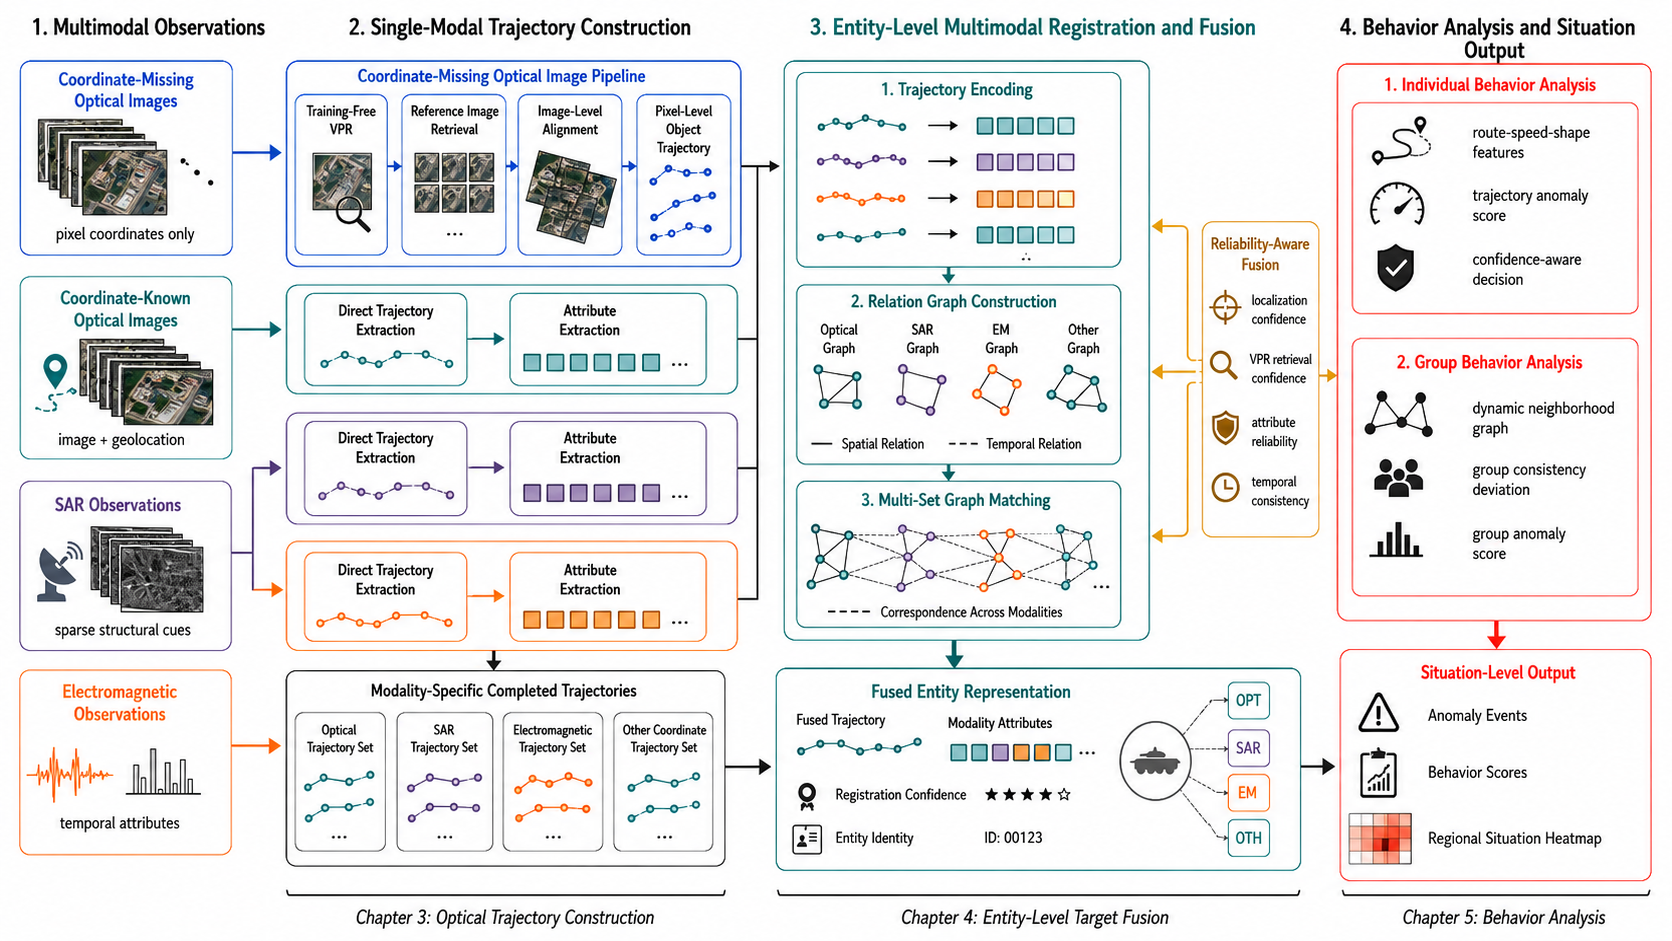
\includegraphics[width=\linewidth]{images/chapter1/overall_technical_route.png}
  \caption{Overall technical route of the proposed multimodal target fusion and behavior analysis system. The pipeline links multimodal observations, single-modal trajectory construction, entity-level registration and fusion, and behavior analysis with situation-level output.}
  \label{fig:intro-technical-route}
\end{figure}

First, corresponding to the single-modal trajectory construction stage in Fig.~\ref{fig:intro-technical-route}, this thesis addresses optical reference retrieval for coordinate-missing images. When reliable geographic coordinates are unavailable, pixel-level target detections cannot be directly transformed into the coordinate frame of existing trajectories. To provide a scene-level access mechanism, this thesis introduces a training-free VPR module based on TF-VPR. The module retrieves coordinate-known reference images for a coordinate-missing query and produces ranked visual reference candidates. These candidates do not serve as direct target-identity decisions; instead, they constrain downstream target association and support optical trajectory access.

Second, corresponding to the entity-level registration and fusion stage in Fig.~\ref{fig:intro-technical-route}, this thesis investigates multimodal target fusion through entity-level registration. After optical observations are connected to the trajectory system, they need to be fused with electromagnetic, SAR, and historical trajectory information. This stage formulates fusion as a cross-modal entity registration problem. Modality-specific trajectories are encoded as target-level representations, graph interaction refines these representations using intra-set structure and cross-set information, and a soft correspondence matrix estimates entity alignments across modalities. The aligned observations are then integrated into unified target trajectories.

Third, corresponding to the behavior analysis and situation output stage in Fig.~\ref{fig:intro-technical-route}, this thesis develops behavior analysis methods for fused multimodal target data. The fused trajectories are used as target-level inputs for individual and group behavior analysis. Individual analysis characterizes route, speed, and shape deviations, whereas group analysis characterizes spatiotemporal consistency, neighborhood variation, splitting, merging, and other relational changes. The outputs include anomaly scores, interpretable event labels, and situation heatmaps.

\subsection{Contributions}
The main contributions of this thesis are summarized as follows.

\begin{enumerate}
  \item This thesis constructs an integrated framework for multimodal target fusion and behavior analysis. The framework links coordinate-missing optical access, cross-modal entity registration, target-level fusion, and behavior anomaly analysis, thereby clarifying the input-output relationships among the main modules and supporting system-level implementation.

  \item This thesis introduces a TF-VPR-based optical reference retrieval strategy for coordinate-missing optical images. The strategy retrieves coordinate-known reference images without additional training on the target scene and uses the resulting candidates to constrain downstream target-level association, thereby reducing dependence on labeled place-recognition data in new scenes.

  \item This thesis designs an entity-level multimodal fusion method based on trajectory representation and graph matching. The method represents modality-specific trajectories as structured entity sets, refines their features through intra-set and cross-set interactions, estimates soft correspondences, and fuses matched observations into unified target trajectories.

  \item This thesis develops a behavior analysis method driven by fused trajectories. The method combines individual anomaly indicators with group-level spatiotemporal consistency analysis, supporting anomaly detection from both single-target motion patterns and multi-target relational changes.
\end{enumerate}

\section{Organization of the Thesis}
The remainder of this thesis is organized as follows.

Chapter 2 presents the overall system architecture and multimodal data modeling. It defines the input data sources, preprocessing flow, unified target representation, and module roles.

Chapter 3 studies optical reference retrieval with TF-VPR. It focuses on coordinate-missing optical images, training-free visual place recognition, and the use of retrieval results for downstream target association.

Chapter 4 studies multimodal target fusion and entity-level registration. It describes trajectory encoding, graph interaction, soft matching, cross-modal correspondence estimation, and entity-level fusion.

Chapter 5 studies behavior analysis based on fused multimodal data. It introduces individual trajectory anomaly scoring, group spatiotemporal consistency analysis, event interpretation, and situation heatmap generation.

Chapter 6 presents system implementation and integrated demonstration. It describes the implementation environment, major modules, data flow, and demonstration workflow.

Chapter 7 concludes the thesis. It summarizes the main research work, discusses limitations, and outlines future directions.

\chapter{System Architecture and Multimodal Data Modeling}

\section{System Design Objectives and Modeling Scope}
Chapter 1 has described the research content and main contributions of this thesis. On that basis, this chapter focuses on the system-level model rather than restating the technical route. Its purpose is to specify how heterogeneous observations are organized before the dedicated methods in later chapters are introduced. Therefore, the emphasis of this section is placed on design objectives, input assumptions, module boundaries, and common data structures.

\begin{enumerate}
  \item Target-centered organization. The system does not directly concatenate raw signals from different sources. Optical images, electromagnetic records, SAR observations, and historical trajectories are first converted into target-level observations or trajectory fragments. This organization keeps the later fusion process focused on physical entities rather than on isolated sensor records.

  \item Missing-data modeling. Different modalities may provide observations at different times and with different spatial references. The model distinguishes coordinate-known observations, coordinate-missing optical images, absent target states, and unreliable detections. The system records such uncertainty through coordinate status, confidence values, and validity masks.

  \item Scene retrieval and target association. For optical images without coordinates, visual reference retrieval can provide coordinate-known scene candidates, but it cannot directly determine target identity. The system design therefore treats retrieval results as constraints for later association, not as final fusion decisions.

  \item Relation-aware representation. Target identity and behavior cannot always be determined from a single target state. The data model must preserve temporal continuity, spatial neighborhoods, and possible cross-modal correspondences. These relations provide the shared basis for entity-level registration and behavior analysis.
\end{enumerate}

Accordingly, the output of this chapter is a system specification rather than an algorithmic contribution. The following sections define the overall architecture, data-source characteristics, coordinate-missing optical access condition, unified target state, modality-specific trajectory set, fused entity form, and spatiotemporal graph representation. These definitions provide a common notation and data interface for the later method chapters.

\section{Overall System Architecture}
The proposed system is organized into six functional layers: multimodal data input, preprocessing, optical reference retrieval, entity-level fusion, behavior analysis, and result presentation. Each layer corresponds to a different level of information abstraction, from raw observations to interpretable situation outputs.

Fig.~\ref{fig:chapter2-layered-architecture} provides the corresponding layered view. It shows how heterogeneous observations are progressively transformed from raw inputs into target records, reference candidates, fused entities, anomaly evidence, and final situation outputs. The figure also indicates the method layers that are developed in Chapters 3, 4, and 5.

\begin{figure}[htb]
  \centering
  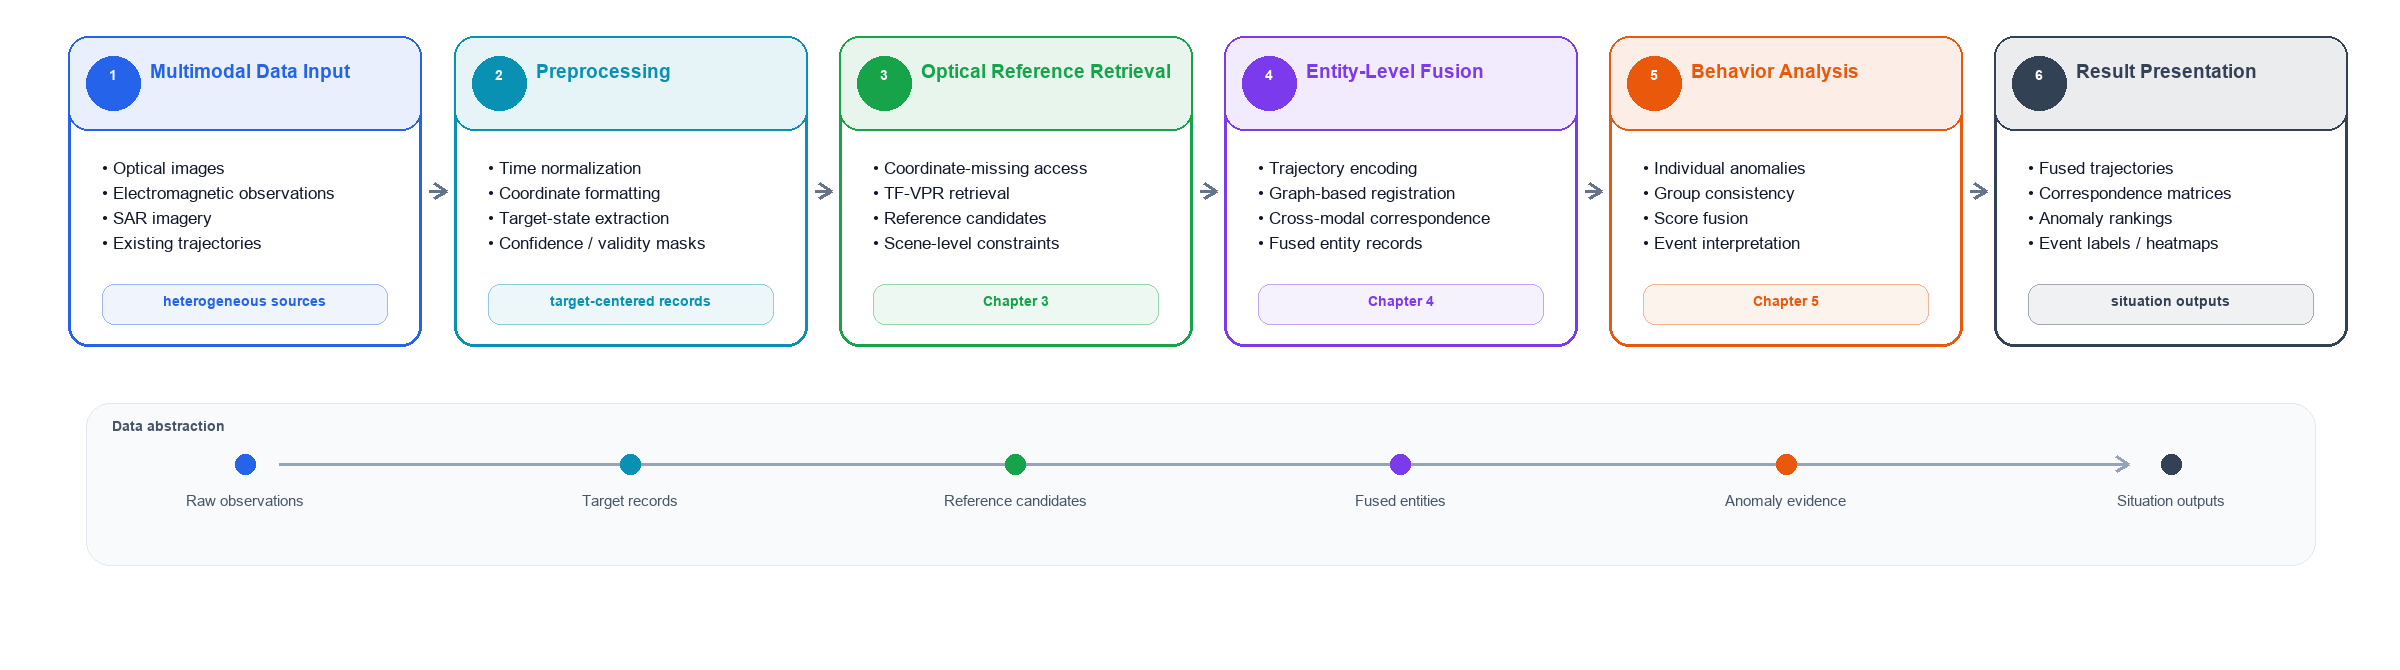
\includegraphics[width=\textwidth]{images/chapter2/chapter2_layered_architecture.png}
  \caption{Layered architecture of the multimodal target fusion and behavior analysis system. Heterogeneous observations are organized through preprocessing, TF-VPR-based optical reference retrieval, entity-level fusion, behavior analysis, and result presentation.}
  \label{fig:chapter2-layered-architecture}
\end{figure}

The multimodal data input layer receives heterogeneous observations. Optical images provide visual appearance, target categories, local image context, and image-plane locations. Electromagnetic observations may provide signal-related or motion-related cues. SAR images provide wide-area sensing under adverse weather or illumination conditions, but their imaging geometry differs from optical imagery. Existing trajectories provide historical target states and temporal continuity. These sources are complementary, but their coordinate systems and feature spaces are not directly compatible.

The preprocessing layer converts raw observations into modality-specific target records. This layer performs time formatting, coordinate normalization, target-state extraction, confidence estimation, missing-value marking, and trajectory organization. Its output is a set of single-modal or partially completed trajectories, rather than the final fused result.

The optical reference retrieval layer handles coordinate-missing optical images. For such images, detected target positions cannot be projected directly into the spatial frame used by other modalities. The system therefore uses TF-VPR to retrieve coordinate-known reference images for each coordinate-missing query. These references provide scene-level constraints for downstream target association.

The entity-level fusion layer estimates whether entities from different modalities correspond to the same physical target. Completed trajectories are first encoded into target-level embeddings. These embeddings are refined through intra-set and cross-set graph interaction, and soft correspondences are then estimated across modality-specific entity sets. Reliable correspondences are used to aggregate trajectory states and modality-specific attributes into fused entity records.

The behavior analysis layer evaluates fused entities. It contains an individual-level detector and a group-level detector. The individual detector measures whether a target's own motion pattern is unusual. The group detector measures whether the target remains consistent with its local group and whether the group undergoes abnormal structural changes. The two sources of evidence are combined into object-level anomaly scores and event decisions.

The result presentation layer converts the system outputs into interpretable records. These records include fused trajectories, cross-modal correspondence matrices, anomaly rankings, event explanations, and situation heatmaps. They support later inspection of both fusion quality and behavior-level situation changes.

After the structural overview in Fig.~\ref{fig:chapter2-layered-architecture}, Table~\ref{tab:chapter2-module-interface} summarizes the interfaces of the main modules. The table describes each module at the system level. Detailed algorithmic designs are presented in Chapters 3, 4, and 5.

\begin{table}[htb]
  \centering
  \caption{Functional interfaces of the main system modules.}
  \label{tab:chapter2-module-interface}
  \setlength{\tabcolsep}{4pt}
  \renewcommand{\arraystretch}{0.95}
  \small
  \begin{tabular}{>{\raggedright\arraybackslash}p{0.20\textwidth}>{\raggedright\arraybackslash}p{0.25\textwidth}>{\raggedright\arraybackslash}p{0.25\textwidth}>{\raggedright\arraybackslash}p{0.22\textwidth}}
    \toprule
    Module & Input & Output & Main function \\
    \midrule
    Multimodal preprocessing & Raw optical, electromagnetic, SAR, and trajectory data & Modality-specific target records & Normalizes format, time, coordinates, attributes, and confidence information \\
    TF-VPR reference retrieval & Coordinate-missing optical image and coordinate-known reference image database & Top-\(k\) reference image candidates & Provides scene-level constraints for optical target association \\
    Target association and trajectory organization & Pixel-level detections and retrieved references & Completed optical trajectory segments & Connects image-plane observations to target or trajectory identifiers \\
    Entity-level registration & Modality-specific trajectory sets & Cross-modal correspondence matrices & Estimates whether entities from different modalities refer to the same physical target \\
    Multimodal fusion & Matched entity groups and correspondence confidence & Fused target records & Aggregates trajectories, attributes, and confidence into unified entities \\
    Behavior analysis & Fused entity trajectories & Anomaly scores, event labels, and heatmaps & Detects individual and group anomalies and supports situation presentation \\
    \bottomrule
  \end{tabular}
\end{table}

\section{Multimodal Data Sources and Feature Analysis}
The system uses several types of input data. Each modality contributes useful information to target understanding, but each also introduces specific uncertainty. Analyzing these properties is necessary before defining the data model.

Optical images provide rich appearance and semantic information. Targets can be described by bounding boxes, centers, local patches, category labels, visual features, and surrounding scene context. Optical data are useful for recognition and visual association. However, they are sensitive to illumination variation, viewpoint change, occlusion, weather, and image quality. Some optical images also lack reliable geographic metadata, which prevents direct comparison with spatial trajectories.

Electromagnetic observation data provide complementary target-related evidence, such as signal characteristics, motion cues, or observation confidence. This modality may be less affected by visual appearance changes. However, it usually has weaker semantic descriptions of target category and local structure. Its feature space may also differ substantially from image-based feature spaces.

SAR imagery provides wide-area and all-weather observation. It can remain informative when optical images are degraded by weather or illumination. However, SAR uses a different imaging mechanism. Target appearance and background structure in SAR images are not directly comparable with optical images. Geometric distortion and speckle noise can further complicate target-level association.

Existing trajectories provide historical target states and temporal continuity. They are important because behavior analysis depends on target evolution over time. Nevertheless, existing trajectories may be incomplete, asynchronous with new observations, or inconsistent with newly detected targets. They may also contain missing segments or identity switches.

These complementary properties motivate target-level multimodal fusion. Optical images provide semantic and appearance cues. Electromagnetic and SAR observations provide additional sensing evidence. Existing trajectories provide temporal context. At the same time, their heterogeneity requires a unified representation and an explicit cross-modal registration mechanism. Table~\ref{tab:chapter2-data-source} summarizes the main properties of the data sources considered in this thesis.

\begin{table}[htb]
  \centering
  \caption{Characteristics of multimodal data sources.}
  \label{tab:chapter2-data-source}
  \small
  \begin{tabular}{p{0.17\textwidth}p{0.25\textwidth}p{0.25\textwidth}p{0.25\textwidth}}
    \toprule
    Data source & Main information & Advantage & Limitation \\
    \midrule
    Optical imagery & Appearance, category, image-plane position, scene context & Rich visual semantics and intuitive target description & Sensitive to illumination, viewpoint, occlusion, weather, and missing geographic metadata \\
    Electromagnetic observation & Signal-related attributes, motion-related cues, observation confidence & Provides complementary non-visual evidence & Weak visual semantics and modality-specific feature space \\
    SAR imagery & Wide-area target response and spatial structure & All-weather and wide-area observation capability & Different imaging geometry, speckle noise, and difficult optical-SAR comparison \\
    Existing trajectories & Historical positions, velocities, and target identities & Provides temporal continuity and prior target context & May be incomplete, asynchronous, or inconsistent with new observations \\
    \bottomrule
  \end{tabular}
\end{table}

From a system-design perspective, these data sources should not be fused directly at the raw-signal level. Their raw forms are too different, and direct concatenation would obscure modality-specific reliability. This thesis therefore adopts target-level fusion. Each modality is first converted into target observations or trajectory fragments. Fusion is then performed after target-level representations have been established.

\section{Existing Trajectories and Coordinate-Missing Optical Images}
The data condition considered in this thesis includes both coordinate-known and coordinate-missing observations. For coordinate-known optical images and other spatially referenced observations, target detections can be projected into a common coordinate frame and linked with existing trajectories through spatial and temporal constraints. By contrast, coordinate-missing optical images provide only pixel-level target observations. These observations cannot be directly compared with trajectories from electromagnetic, SAR, or historical sources. Therefore, an additional access mechanism is required to connect image-plane observations to the existing trajectory system.

As illustrated in Fig.~\ref{fig:chapter2-optical-access}, the access mechanism separates scene-level reference retrieval from target-level association. TF-VPR retrieves coordinate-known reference candidates for a coordinate-missing query and thereby narrows the candidate search space. The downstream association module then uses the pixel-level detections, retrieved references, and existing trajectory records to estimate target-level correspondence and generate an optical trajectory segment or association record.

\begin{figure}[htb]
  \centering
  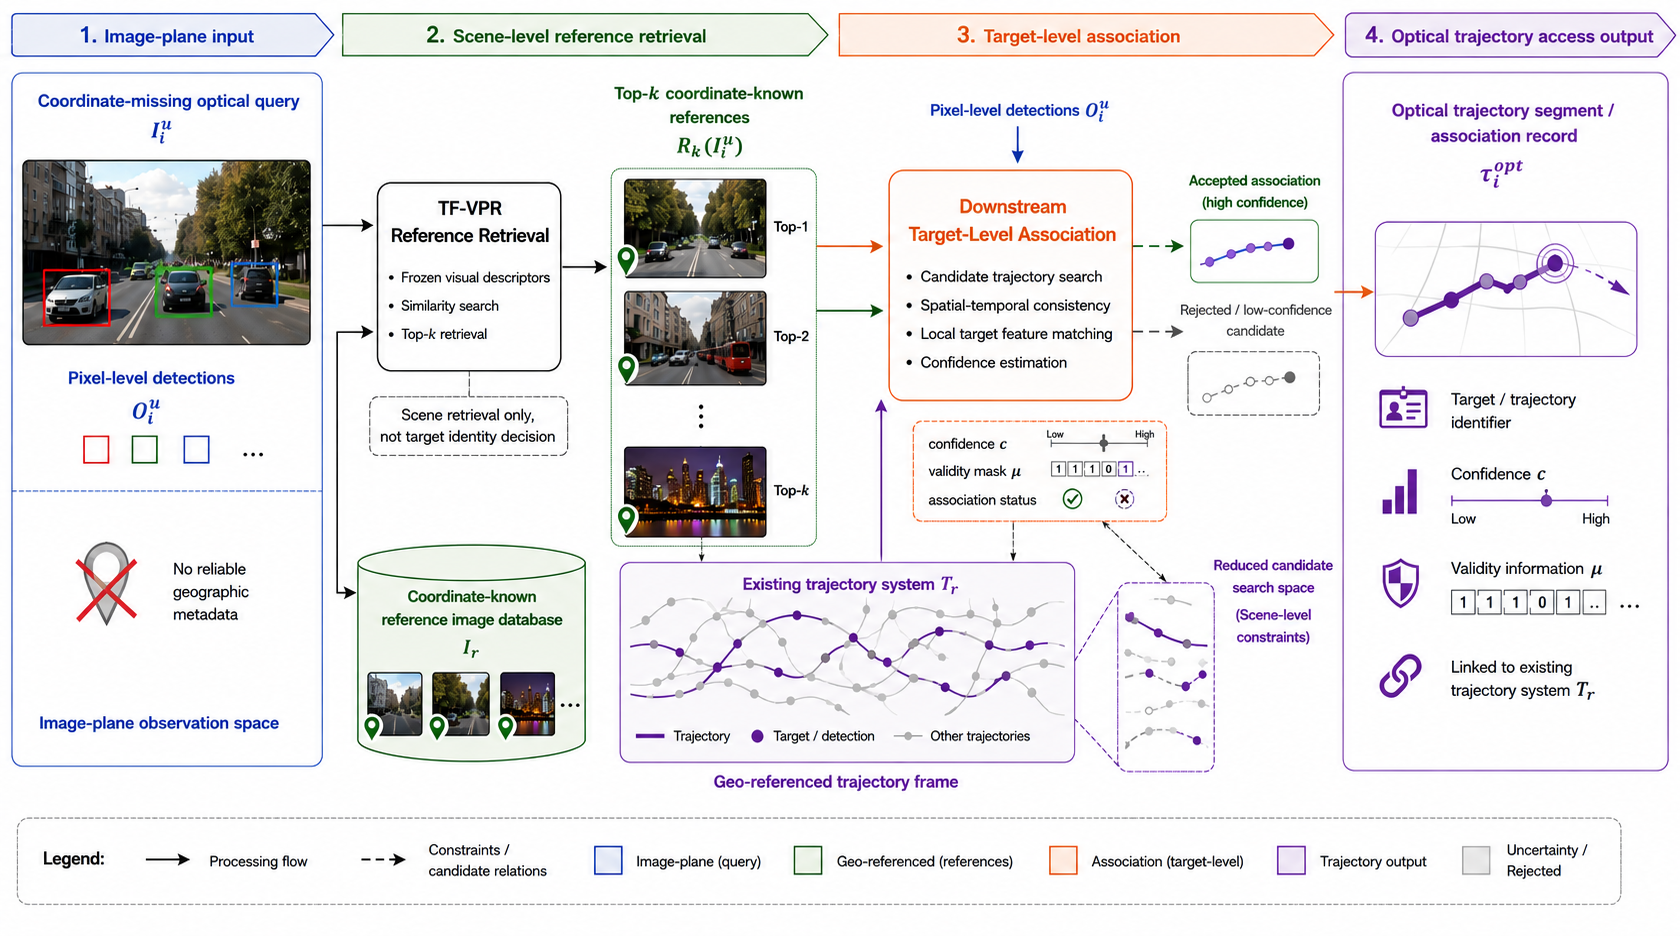
\includegraphics[width=\textwidth,height=0.42\textheight,keepaspectratio]{images/chapter2/coordinate_missing_optical_access.png}
  \caption{Coordinate-missing optical access mechanism. TF-VPR provides scene-level coordinate-known reference candidates for coordinate-missing optical queries, while the downstream association module uses these candidates to constrain target-level trajectory association and output an optical trajectory segment or association record.}
  \label{fig:chapter2-optical-access}
\end{figure}

Consistent with the notation in Fig.~\ref{fig:chapter2-optical-access}, let \(I_u=\{I^u_1,I^u_2,\ldots,I^u_{N_u}\}\) denote the set of coordinate-missing optical images, where \(N_u\) is the number of such images. Let \(I_r=\{I^r_1,I^r_2,\ldots,I^r_{N_r}\}\) denote the coordinate-known optical reference database, where \(N_r\) is the number of reference images. For the \(i\)-th coordinate-missing image \(I^u_i\), a target detector can provide pixel-level observations
\begin{equation}
  O^u_i = \{o^u_{i,1},o^u_{i,2},\ldots,o^u_{i,n_i}\},
\end{equation}
where \(O^u_i\) is the observation set of image \(I^u_i\), \(o^u_{i,l}\) is the \(l\)-th detected target observation in that image, and \(n_i\) is the number of detected target observations. Each observation may include a bounding box, a target center, a category label, and a local target feature. Without a geographic reference, \(O^u_i\) cannot be directly mapped into the spatial trajectory set.

The system therefore first performs image-level reference retrieval:
\begin{equation}
  \mathcal{R}_k(I^u_i)
  =
  \operatorname{TopK}_{I^r_j\in I_r}
  \operatorname{sim}\big(g(I^u_i),g(I^r_j)\big),
\end{equation}
where \(g(\cdot)\) denotes the image descriptor generated by TF-VPR. The function \(\operatorname{sim}(\cdot,\cdot)\) denotes descriptor similarity. The retrieved set \(\mathcal{R}_k(I^u_i)\) contains the top-\(k\) coordinate-known references that are visually related to the query.
Here, \(k\) is the number of retained reference candidates, and \(\operatorname{TopK}_{I^r_j\in I_r}\) returns the \(k\) reference images with the highest similarity scores among all \(I^r_j\) in \(I_r\).

The retrieval result is a scene-level constraint, not a final target-level association. A high image similarity score indicates that the query and reference images are visually related. It does not prove that a detected target in the query corresponds to a specific target in the reference data. As shown by the constraint path in Fig.~\ref{fig:chapter2-optical-access}, the retrieved references are therefore used to reduce the search space for downstream association. The target association module then compares pixel-level detections, local target features, temporal consistency, and candidate trajectory states within this constrained set.

After target association, coordinate-missing optical observations can be converted into optical trajectory segments or association records:
\begin{equation}
  \tau^{\mathrm{opt}}_a
  =
  \{x^{\mathrm{opt}}_{a,t_1},x^{\mathrm{opt}}_{a,t_2},\ldots,x^{\mathrm{opt}}_{a,t_{L_a}}\}.
\end{equation}
Here, \(a\) indexes an associated optical target, \(t_1,\ldots,t_{L_a}\) are the time stamps of the segment, \(L_a\) is the segment length, and \(x^{\mathrm{opt}}_{a,t}\) is the optical target state at time \(t\). This output corresponds to the optical trajectory access result in Fig.~\ref{fig:chapter2-optical-access}. These segments do not need to be perfect before entering the fusion stage. They provide target-level evidence with explicit confidence and validity information. Chapter 4 then combines this optical evidence with other modalities and suppresses unreliable correspondences through relation-aware matching.

This design has two advantages. First, it avoids assuming that every optical image has accurate geographic metadata. Second, it separates image-level scene retrieval from target-level identity association. TF-VPR locates candidate reference scenes without additional scene-specific training. The downstream association module then focuses on target correspondence within a smaller candidate space.

\section{Multimodal Data Preprocessing and Unified Representation}
Before multimodal fusion, observations from different sources must be converted into a common target-centered format. The purpose of preprocessing is not to remove modality differences. Instead, it organizes heterogeneous information so that it can be compared, registered, and fused at the entity level.

The preprocessing stage contains four basic operations. First, time stamps are normalized to a common temporal reference. When modalities have different sampling rates, each observation is assigned to a discrete time index or interval. Second, spatial information is formatted consistently. Coordinate-known observations are represented in the spatial frame when possible. Coordinate-missing optical observations remain in the image plane until they are connected to reference trajectories. Third, modality-specific attributes are extracted and stored without forcing them into identical feature dimensions. Fourth, missing observations and uncertainty are recorded through masks and confidence scores.

For modality \(m\), the target state of entity \(i\) at time \(t\) is represented as
\begin{equation}
  x_{i,t}^{(m)}
  =
  \big[
  p_{i,t}^{(m)},\,
  v_{i,t}^{(m)},\,
  f_{i,t}^{(m)},\,
  c_{i,t}^{(m)},\,
  \mu_{i,t}^{(m)}
  \big],
  \label{eq:chapter2-target-state}
\end{equation}
where \(p_{i,t}^{(m)}\) denotes position information, \(v_{i,t}^{(m)}\) denotes motion information, and \(f_{i,t}^{(m)}\) denotes modality-specific attributes. The term \(c_{i,t}^{(m)}\) denotes observation confidence, and \(\mu_{i,t}^{(m)}\) denotes the validity mask.

The position term \(p_{i,t}^{(m)}\) may have different meanings before and after reference connection. For spatially referenced observations, it represents a position in the common coordinate frame. For coordinate-missing optical images before association, it may represent an image-plane center or bounding-box position. After TF-VPR-based retrieval and target association, optical observations can be linked to candidate trajectory identifiers and used in the fusion stage.

The motion term \(v_{i,t}^{(m)}\) describes target dynamics, such as velocity, displacement, or direction. It can be computed from consecutive positions when raw velocity is unavailable. The attribute term \(f_{i,t}^{(m)}\) preserves modality-specific information, including optical appearance features, electromagnetic attributes, SAR response descriptors, or historical trajectory descriptors. The confidence term \(c_{i,t}^{(m)}\) records observation reliability. The mask term \(\mu_{i,t}^{(m)}\in\{0,1\}\) indicates whether modality \(m\) provides a valid observation for target \(i\) at time \(t\).

Based on Eq.~\eqref{eq:chapter2-target-state}, a modality-specific trajectory is written as
\begin{equation}
  \tau_i^{(m)}
  =
  \{x_{i,t_1}^{(m)},x_{i,t_2}^{(m)},\ldots,x_{i,t_L}^{(m)}\},
\end{equation}
and the trajectory set of modality \(m\) is written as
\begin{equation}
  \mathcal{T}^{(m)}
  =
  \{\tau_1^{(m)},\tau_2^{(m)},\ldots,\tau_{N_m}^{(m)}\}.
\end{equation}
Here, \(\tau_i^{(m)}\) denotes the trajectory of entity \(i\) in modality \(m\), \(t_1,t_2,\ldots,t_L\) denote the ordered time stamps of the trajectory, and \(L\) denotes the number of states in the trajectory. The set \(\mathcal{T}^{(m)}\) contains all modality-\(m\) trajectories, and \(N_m\) denotes the number of trajectories in this modality.

This representation has three functions. First, it allows all modalities to share a target-level structure while preserving modality-specific attributes. Second, it avoids treating missing data as ordinary numerical values. Missing observations are explicitly marked by \(\mu_{i,t}^{(m)}\). Third, it provides the input interface for entity-level registration in Chapter 4 and behavior analysis in Chapter 5.

After cross-modal registration and fusion, the final fused entity can be represented as
\begin{equation}
  e_j = \{T_j,F_j,C_j\},
\end{equation}
where \(e_j\) denotes the \(j\)-th fused entity, \(T_j\) denotes its fused trajectory component, \(F_j\) denotes its fused multimodal attribute component, and \(C_j\) denotes its confidence information. Chapter 4 describes how this fused representation is generated. In this chapter, the key point is that Eq.~\eqref{eq:chapter2-target-state} defines the data basis from which fused entities are constructed.

\section{Spatiotemporal Graph Construction}
Target fusion and behavior analysis both require relational information. A target cannot always be identified by local attributes alone, especially when different modalities use different feature spaces. Similarly, abnormal behavior cannot always be detected from one trajectory alone. Many abnormal events are defined by the relation between a target and its surrounding group. The system therefore organizes preprocessed target records as spatiotemporal graphs.

At time \(t\), visible target states are treated as graph nodes:
\begin{equation}
  \mathcal{V}_t
  =
  \{z_{i,t}\mid \mu_{i,t}=1\}.
\end{equation}
Here, \(z_{i,t}\) denotes the graph node corresponding to target \(i\) at time \(t\), and \(\mu_{i,t}\) denotes the validity mask of the corresponding target state. When the graph is built for a specific modality, the superscript \((m)\) in \(\mu_{i,t}^{(m)}\) is omitted for readability. Each node stores the target-centered state in Eq.~\eqref{eq:chapter2-target-state}, or a feature embedding derived from that state. The graph contains three types of edges: temporal edges, spatial edges, and cross-modal candidate edges.

Temporal edges connect observations or states that belong to the same target across adjacent time steps:
\begin{equation}
  \mathcal{E}^{\mathrm{time}}
  =
  \{(z_{i,t},z_{i,t+1})\mid z_{i,t}\in\mathcal{V}_t,\ z_{i,t+1}\in\mathcal{V}_{t+1}\}.
\end{equation}
These edges preserve trajectory continuity and support later motion modeling. In this formula, the same target index \(i\) indicates that the two nodes belong to the same target at adjacent time steps.

Spatial edges connect targets that are close in position, motion, or local context within the same time step:
\begin{equation}
  \mathcal{E}^{\mathrm{space}}_t
  =
  \{(z_{i,t},z_{j,t})\mid j\in\mathcal{N}_K(i,t)\},
\end{equation}
where \(\mathcal{N}_K(i,t)\) denotes the \(K\)-nearest neighbors of target \(i\) at time \(t\), \(j\) denotes a neighboring target index, and \(K\) is the preset neighborhood size. The neighborhood can be defined by spatial distance, motion similarity, category consistency, confidence, or a combination of these factors. These edges provide the structural basis for group behavior modeling in Chapter 5.

Cross-modal candidate edges connect entities from different modalities when they may correspond to the same physical target:
\begin{equation}
  \mathcal{E}^{\mathrm{cross}}
  =
  \{(\tau_i^{(m)},\tau_j^{(n)})\mid m\neq n,\ \operatorname{comp}(\tau_i^{(m)},\tau_j^{(n)})>\delta\},
\end{equation}
where \(m\) and \(n\) are two different modality indices, \(i\) and \(j\) are trajectory indices within the corresponding modalities, and \(\operatorname{comp}(\cdot,\cdot)\) denotes a compatibility score based on temporal overlap, spatial consistency, attribute similarity, and confidence. The threshold \(\delta\) defines the candidate relation set. These edges do not impose final identity decisions. They only define plausible cross-modal relations to be refined by the registration method in Chapter 4.

The graph representation can be written as
\begin{equation}
  \mathcal{G}
  =
  (\mathcal{V},\mathcal{E}^{\mathrm{time}},\mathcal{E}^{\mathrm{space}},\mathcal{E}^{\mathrm{cross}}).
\end{equation}
In this representation, \(\mathcal{G}\) denotes the spatiotemporal graph, \(\mathcal{V}=\bigcup_t\mathcal{V}_t\) denotes the complete node set over all time steps, and \(\mathcal{E}^{\mathrm{space}}=\bigcup_t\mathcal{E}^{\mathrm{space}}_t\) denotes all spatial edges. Temporal edges describe target evolution, spatial edges describe target interaction, and cross-modal edges describe possible identity correspondences.

The graph is used differently in later chapters. In Chapter 4, graph interaction supports entity-level registration. Modality-specific entity sets are refined through intra-set and cross-set interaction, and the resulting features are used to estimate soft correspondence matrices. In Chapter 5, the graph supports behavior analysis. Spatial and temporal edges describe group structure and motion evolution, while abnormal behavior is detected from prediction errors and interpretable group-event indicators.

The spatiotemporal graph defined here is therefore a system-level data structure rather than a single fixed algorithm. It provides a common relational representation for multimodal fusion and behavior understanding.

\section{Chapter Summary}
This chapter presented the system architecture and data modeling strategy of the proposed multimodal target fusion and behavior analysis framework. The system was organized as a staged pipeline from heterogeneous data input to fused entity representation and behavior analysis output. The chapter also clarified the role of multimodal preprocessing, TF-VPR-based optical reference retrieval, target association, entity-level registration, multimodal fusion, and behavior analysis.

The chapter analyzed the characteristics of optical, electromagnetic, SAR, and existing trajectory data. Their complementary advantages motivate multimodal fusion, but their differences in coordinate systems, sampling rates, feature spaces, and uncertainty require a unified target-level representation. For coordinate-missing optical images, the chapter explained why image-level reference retrieval is needed before target-level association, and why TF-VPR is used as the retrieval module.

Finally, this chapter defined a target-centered state representation and a spatiotemporal graph structure for temporal continuity, spatial neighborhoods, and cross-modal candidate correspondences. These definitions provide the data interface for Chapter 3's TF-VPR retrieval, Chapter 4's entity-level fusion, and Chapter 5's behavior analysis.

\chapter{Optical Reference Retrieval with TF-VPR}

\section{Introduction}
Coordinate-missing optical images are difficult to use directly in a multimodal trajectory system. Images with geographic coordinates can be associated with trajectories through their spatial and temporal metadata, while coordinate-missing images only provide visual observations and pixel-level target information. Before these observations can participate in multimodal fusion, the system must first identify visually related coordinate-known references and use them as scene-level anchors.

Visual place recognition provides a natural technical route for this problem. However, as emphasized in the TF-VPR work \cite{wang2026tfvpr}, most strong VPR systems are built around training-intensive pipelines. Single-stage methods learn compact global descriptors for nearest-neighbor retrieval, and two-stage methods combine coarse global retrieval with local feature matching or geometric verification. Although these paradigms are effective, they usually require annotated place pairs, task-specific loss design, hard-negative mining, and large-scale optimization. Such assumptions are not suitable for the coordinate-missing optical setting considered in this thesis, where new scenes may lack reliable place labels and additional VPR training data.

Recent vision foundation models provide a different opportunity. Models such as CLIP, ViT, MAE, and DINOv2 contain transferable visual representations learned from large-scale pretraining. Instead of fine-tuning these models for every new scene, TF-VPR investigates a training-free paradigm in which descriptors are generated, refined, and matched only at test time. This paradigm reduces dependence on annotated datasets, avoids scene-specific optimization, and enables direct reuse of frozen visual features.

Following this idea, this chapter uses TF-VPR as the optical reference retrieval module in the proposed trajectory completion framework. The module retrieves coordinate-known reference images for each coordinate-missing optical image. These retrieved references do not directly produce an absolute geographic trajectory; rather, they provide a constrained candidate set for the downstream target association model. The target association model then links pixel-level target observations to existing target or trajectory identifiers.

Therefore, the contribution of this chapter is not to propose a new target-level matching network, but to organize a training-free optical reference retrieval process that bridges coordinate-missing optical observations and the multimodal fusion pipeline. The following sections define the retrieval problem, describe the TF-VPR-based descriptor generation and Top-\(k\) retrieval process, and explain how the retrieved references are integrated with downstream target association.

\section{Related Work}
This section extends the brief overview of visual place recognition in Chapter 1 and focuses on the literature most relevant to the optical reference retrieval module. The discussion is organized around four lines of work: conventional VPR, graph-based VPR, VFM-based VPR, and training-free visual adaptation.

\subsection{Visual Place Recognition}
Visual place recognition (VPR) determines whether a query image depicts a previously observed place. It is a core component of robotic localization, loop-closure detection, long-term navigation, and large-scale visual retrieval \cite{yin2025gprs,murartal2017orbslam2,milford2008seqslam}. Unlike generic image retrieval, VPR must remain reliable under viewpoint changes, illumination variation, seasonal shifts, occlusion, dynamic objects, and domain shift. These factors are also present in the optical images studied in this thesis, especially when images are collected under different observation conditions or lack reliable geographic coordinates.

Early VPR methods relied mainly on hand-crafted local features and aggregation strategies, including Bag-of-Words and VLAD \cite{galvez2012bags,jegou2010vlad}. These methods are computationally efficient and easy to deploy, but their representation capacity is limited under large appearance changes. With the development of deep learning, CNN-based and Transformer-based methods have become the dominant approach. Existing VPR pipelines can be broadly divided into single-stage and two-stage paradigms \cite{wang2026tfvpr}.

As shown in Fig.~\ref{fig:tfvpr-single-stage-vpr}, single-stage methods encode each image into a compact global descriptor and retrieve reference images through nearest-neighbor search. NetVLAD introduced a learnable VLAD-style aggregation layer for weakly supervised place recognition \cite{arandjelovic2016netvlad}. Patch-NetVLAD further improved retrieval by combining local and global descriptors at multiple scales \cite{hausler2021patchnetvlad}. More recent methods, including CosPlace, EigenPlaces, and MixVPR, improve descriptor discriminability through better training data construction, viewpoint-robust learning, and feature mixing \cite{berton2022cosplace,berton2023eigenplaces,alibey2023mixvpr}.

Two-stage VPR pipelines use a coarse-to-fine retrieval process. As illustrated in Fig.~\ref{fig:tfvpr-two-stage-vpr}, a global descriptor first retrieves candidate reference images, and local feature matching or geometric verification then reranks these candidates. This design can improve robustness under viewpoint and structural changes by combining global scene-level cues with local spatial correspondences. However, both single-stage and two-stage learning-based paradigms often rely on annotated training data, task-specific losses, and hard-negative mining. These requirements are restrictive in newly observed scenes where coordinate labels, place correspondences, or retrieval annotations are unavailable. For the coordinate-missing optical setting in this thesis, the retrieval module must therefore operate without additional scene-specific VPR training.

\begin{figure}[!htbp]
  \centering
  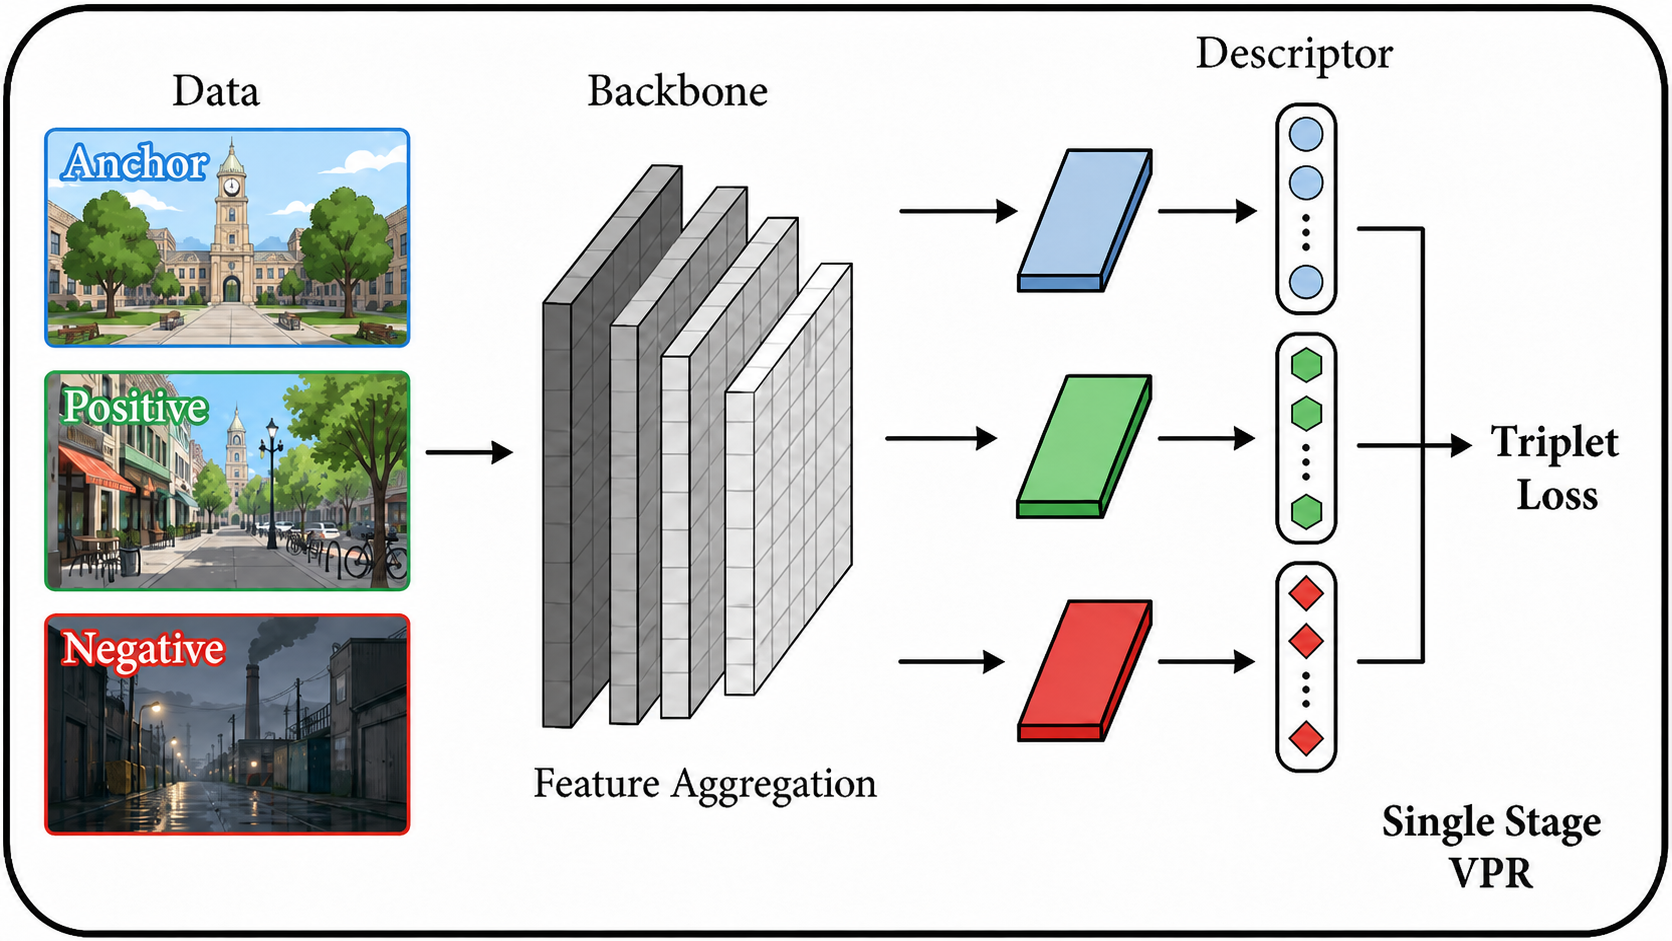
\includegraphics[width=0.88\linewidth,height=0.28\textheight,keepaspectratio]{images/chapter3/single_stage_vpr_pipeline.png}
  \caption{Single-stage VPR pipeline. A query image is encoded by a backbone into a compact global descriptor, and reference images are retrieved by nearest-neighbor search \cite{arandjelovic2016netvlad,hausler2021patchnetvlad}.}
  \label{fig:tfvpr-single-stage-vpr}
\end{figure}

\begin{figure}[!htbp]
  \centering
  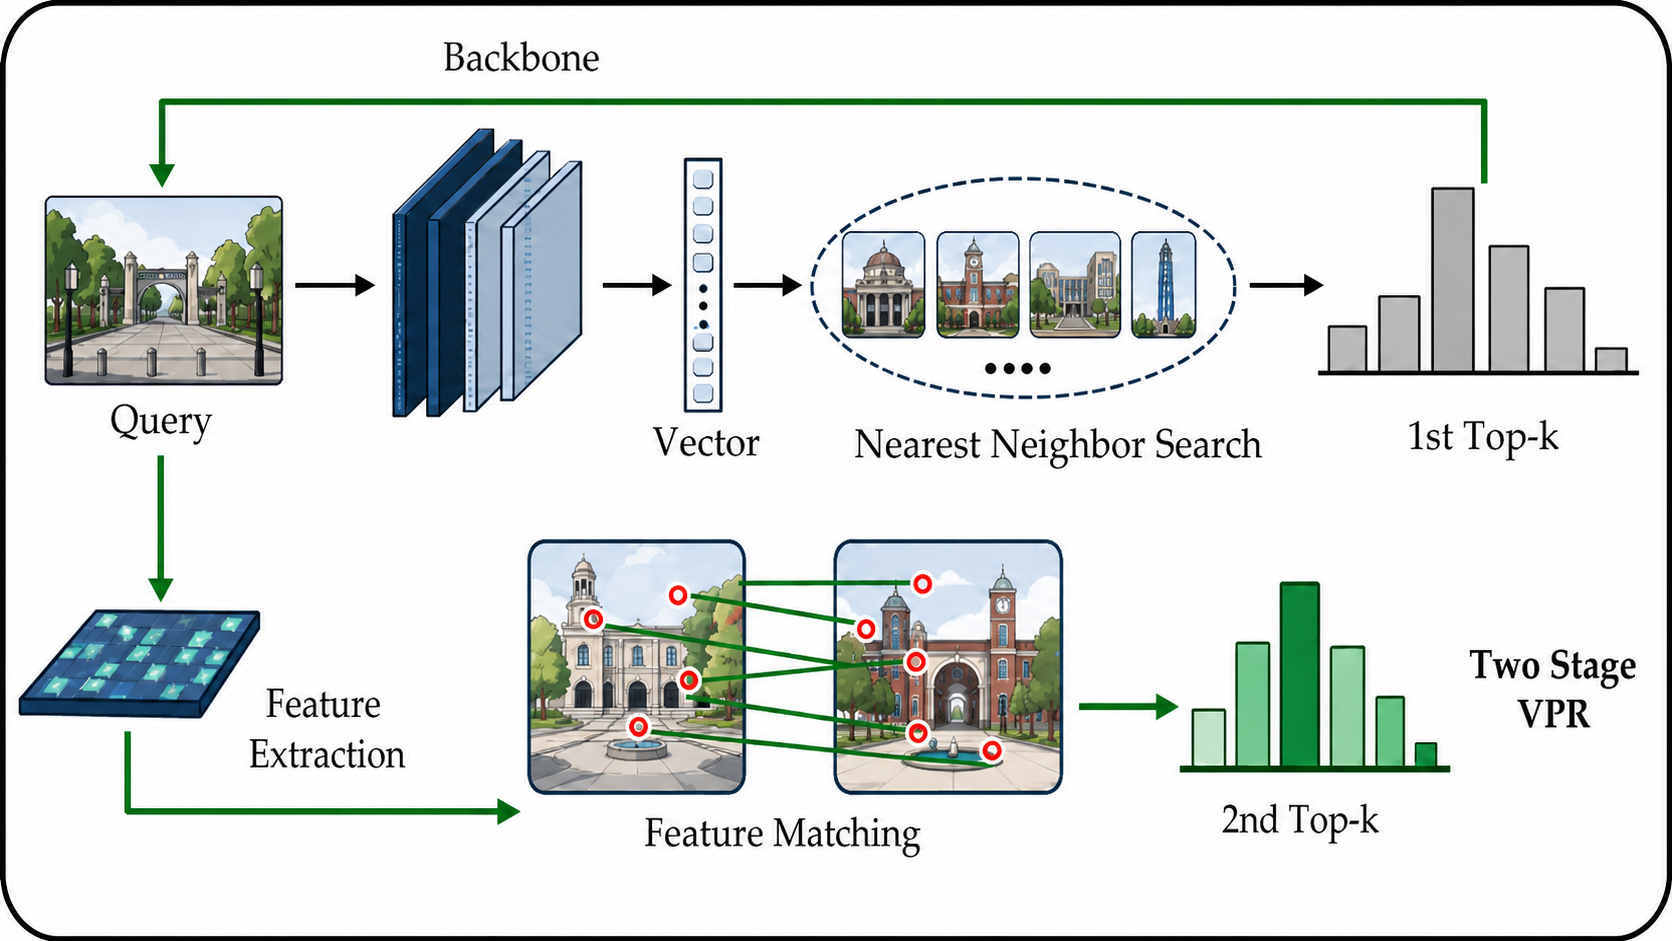
\includegraphics[width=0.88\linewidth,height=0.28\textheight,keepaspectratio]{images/chapter3/two_stage_vpr_pipeline.png}
  \caption{Two-stage VPR pipeline. A global descriptor first retrieves candidate references, and local feature matching then reranks the candidates to obtain a refined Top-k result for more reliable place recognition.}
  \label{fig:tfvpr-two-stage-vpr}
\end{figure}

\subsection{Graph-Based Visual Place Recognition}
Graph-based VPR methods improve retrieval robustness by modeling spatial or semantic relationships among image regions. Rather than treating an image descriptor as a single pooled vector, these methods represent patches, regions, or semantic components as graph nodes and use their relationships for place matching. Qin et al. use learnable feature-map filtering and graph attention networks to model dependencies among feature regions \cite{qin2021gatvpr}. PRGS introduces patch-to-region graph search to improve robustness under viewpoint variation \cite{zuo2025prgs}. SAGE further combines spatial-visual graph exploration with parameter-efficient fine-tuning and dynamic hard-sample mining \cite{chen2025sage}.

These studies show that graph reasoning is useful for VPR because stable spatial structures are often more reliable than isolated visual responses. However, most graph-based VPR methods still require task-specific training or fine-tuning. This limits their direct applicability to coordinate-missing optical images, where labeled VPR pairs may not exist. The TF-VPR strategy adopted in this chapter retains the structural motivation of graph-based VPR while avoiding learned graph parameters. Its Training-Free Graph-Attention Module constructs token relationships directly from frozen visual features and performs parameter-free feature refinement. This makes graph reasoning more suitable for deployment without scene-specific annotation.

\subsection{VFM-Based Visual Place Recognition}
Vision foundation models (VFMs), including CLIP, ViT, MAE, and DINOv2, have shown strong general visual representation ability through large-scale pretraining \cite{radford2021clip,dosovitskiy2020vit,he2022mae,oquab2023dinov2}. Their emergence creates a practical opportunity for VPR. Instead of training a place recognition model from scratch, one can reuse frozen visual representations and evaluate how well they support place retrieval. AnyLoc is a representative training-free VFM-based VPR method. It applies off-the-shelf DINOv2 features with pooling strategies such as GeM or VLAD \cite{keetha2024anyloc}. Its results indicate that frozen VFM features can provide strong zero-shot place recognition across diverse environments.

Simple pooling over frozen VFM tokens, however, may not fully exploit spatial structure or cross-image alignment. In contrast, SALAD introduces an optimal-transport-based aggregation strategy and a dustbin cluster to suppress distractors, including sky regions and dynamic objects, but it requires training or fine-tuning \cite{izquierdo2024salad}. This contrast defines a methodological gap. Training-free VFM features are flexible and annotation-efficient, whereas trained aggregation modules often produce stronger descriptors but reduce deployment flexibility. TF-VPR is positioned in this gap. It keeps the backbone frozen, as in training-free VFM-based methods, and introduces deterministic attention-based refinement to improve descriptor discriminability without additional training \cite{wang2026tfvpr}.

\subsection{Training-Free Visual Adaptation}
Training-free methods in related visual tasks provide useful inspiration for TF-VPR. In training-free segmentation and open-vocabulary dense prediction, frozen foundation models are adapted at inference time by manipulating token interactions, attention maps, or prototype representations rather than updating model parameters. Methods such as MaskCLIP and CLIP-based dense prediction show that frozen vision-language or visual backbones already encode useful dense semantics, although their raw attention responses may contain noise or spatial inconsistency \cite{ding2023maskclip,sun2024clipasrnn}. These observations suggest that performance can often be improved by refining how frozen features are read and aggregated, even when model weights remain unchanged.

Zero-shot classification methods provide another related perspective. Parameter-free attention, non-parametric memory, and test-time calibration strategies can improve the use of frozen features without supervised fine-tuning \cite{guo2023calip,zanella2024testtime}. These ideas are compatible with the deployment requirement of this thesis. The system should process coordinate-missing optical images from new scenes without constructing an additional labeled training set. Therefore, the focus shifts from learning new parameters to extracting, refining, and comparing frozen visual features in a deterministic and reproducible way.

Based on this literature, this chapter adopts TF-VPR as the optical reference retrieval module. As summarized in Fig.~\ref{fig:tfvpr-training-free-benchmark}, its key difference from training-based VPR is that descriptor generation uses a frozen backbone and deterministic aggregation at test time. It does not optimize the backbone or aggregation module on a dedicated VPR training set. The module uses frozen VFM representations and training-free attention mechanisms to retrieve coordinate-known reference images for coordinate-missing optical images. These retrieved references then constrain downstream target association, which links pixel-level observations to target or trajectory identifiers. In this chapter, TF-VPR is used primarily as a scene-level candidate retrieval stage, while target-level correspondence is handled by the downstream association module. In this way, TF-VPR provides the retrieval bridge between coordinate-missing optical images and the multimodal target fusion module developed in the next chapter.

\begin{figure}[!htbp]
  \centering
  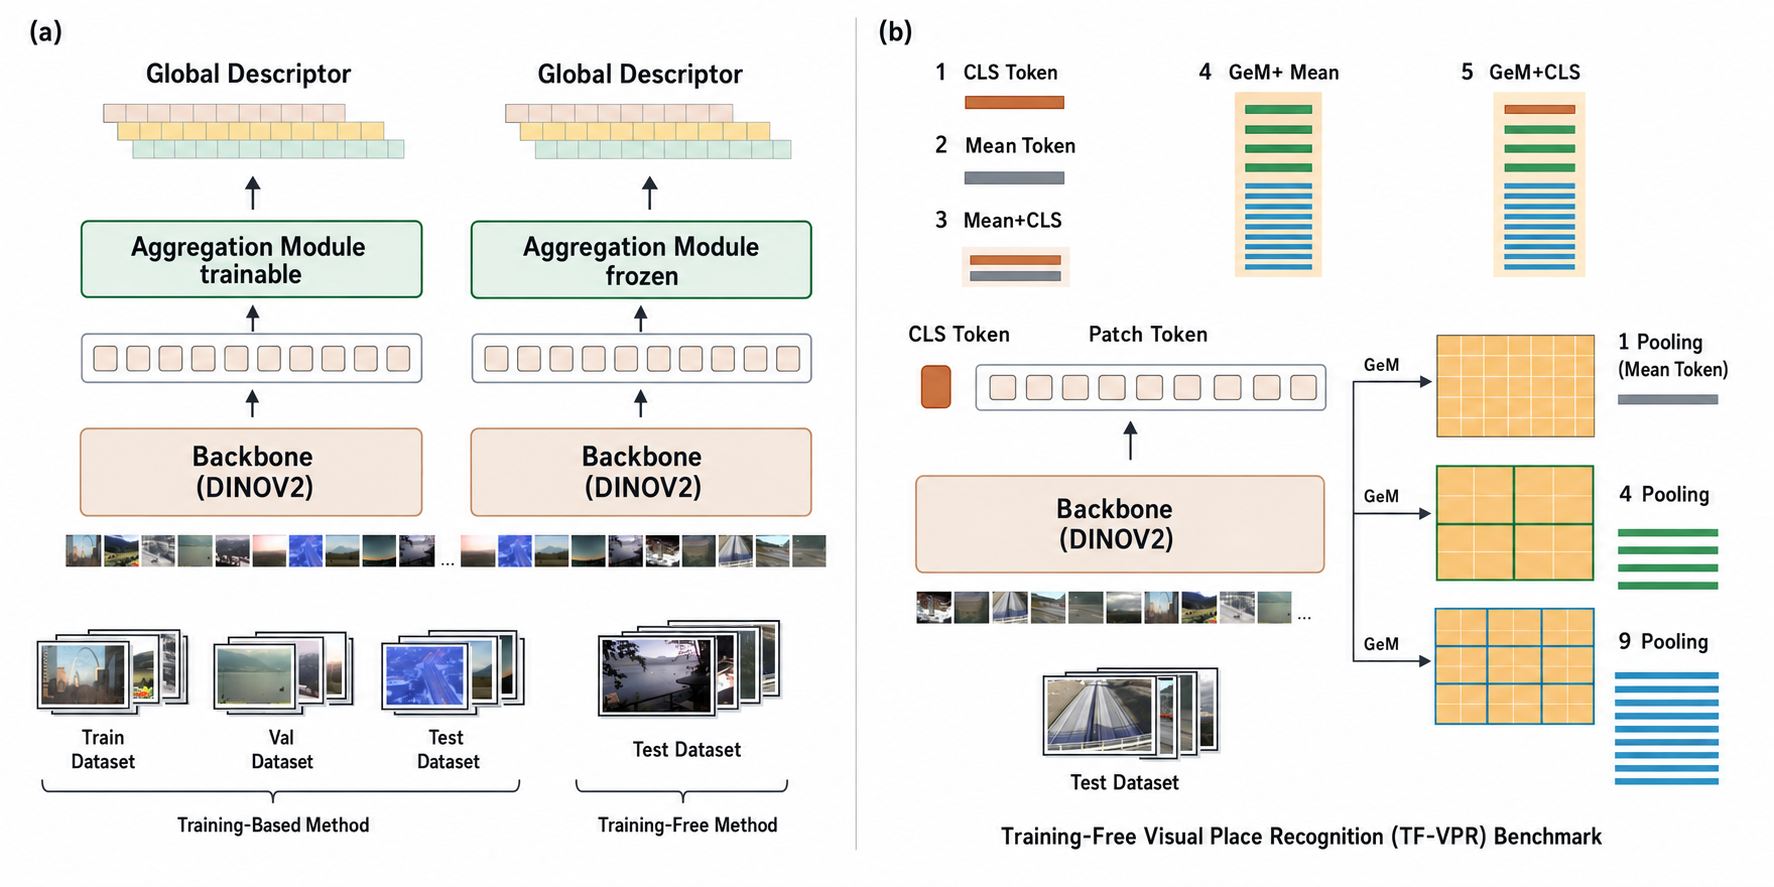
\includegraphics[width=\linewidth,height=0.38\textheight,keepaspectratio]{images/chapter3/tf_vpr_overview.png}
  \caption{Training-free VPR motivation and descriptor benchmark. TF-VPR differs from training-based VPR by keeping the DINOv2 backbone and aggregation process fixed during deployment, and it compares several frozen-token aggregation choices such as CLS, mean, and GeM-based descriptors \cite{wang2026tfvpr}.}
  \label{fig:tfvpr-training-free-benchmark}
\end{figure}

\section{Problem Definition}
Let \(I_u\) denote a set of coordinate-missing optical images, and let \(I_r\) denote a set of coordinate-known reference optical images. The existing trajectory set is denoted as \(T_r\), which may be obtained from coordinate-known optical images or other sensing modalities. For each image in \(I_u\), pixel-level target observations are denoted as \(O_u\), including target boxes, target centers, or local target patches.

The objective of this chapter is to retrieve reliable reference images from \(I_r\) for each coordinate-missing image in \(I_u\), and then use downstream target association results to connect \(O_u\) to the existing trajectory system. The output of this chapter is not an absolute geographic trajectory recovered directly from pixels. Instead, the output is a trajectory association record or a completed optical trajectory segment that can be used by the multimodal fusion module in the next chapter.

\section{TF-VPR Method}
The TF-VPR module is responsible for image-level candidate reference retrieval. It generates image descriptors from a frozen vision foundation model and refines them using training-free attention mechanisms. Since no additional training or fine-tuning is required, the module is suitable for scenes where labeled VPR training data are unavailable. The overall pipeline is shown in Fig.~\ref{fig:tfvpr-method-framework}: the frozen backbone first extracts patch tokens, TF-GAM refines them through graph-style propagation, TF-CAM aggregates them with prototype-guided cross-attention, and the resulting global descriptor is used for image-level retrieval.

\begin{figure}[!htbp]
  \centering
  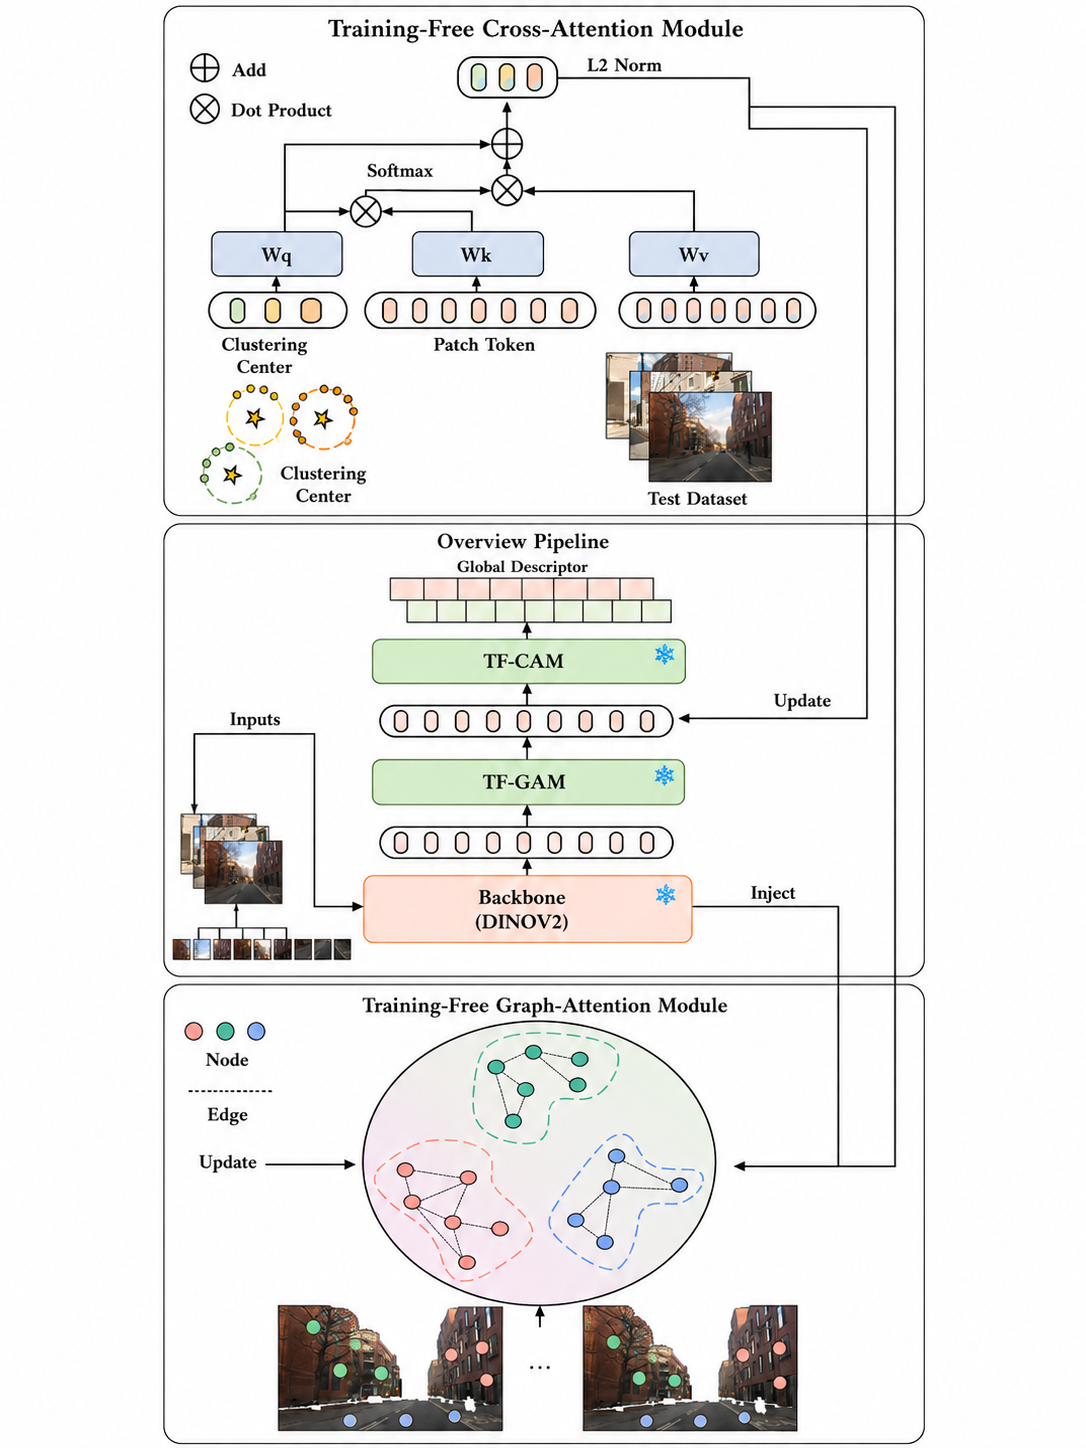
\includegraphics[width=\linewidth,height=0.40\textheight,keepaspectratio]{images/chapter3/tf_vpr_method.png}
  \caption{TF-VPR framework. The method combines frozen DINOv2 feature extraction, a Training-Free Graph-Attention Module, and a Training-Free Cross-Attention Module to generate global descriptors for training-free visual place recognition \cite{wang2026tfvpr}.}
  \label{fig:tfvpr-method-framework}
\end{figure}

\subsection{Training-Free VPR Framework}
Given an input image, a frozen visual encoder extracts a class token and a set of patch tokens. These features are used to build an image descriptor through deterministic operations. Unlike training-based VPR methods, the backbone parameters remain fixed, and all descriptor generation, refinement, and matching operations are performed at inference time.

More specifically, following the TF-VPR formulation \cite{wang2026tfvpr}, let \(f_{\theta}\) denote a pretrained visual foundation model with fixed parameters \(\theta\). For an image \(I\), the backbone outputs a class token \(x_{\mathrm{cls}} \in \mathbb{R}^{d}\) and \(N\) patch tokens:
\begin{equation}
  X = [x_1; x_2; \ldots; x_N] \in \mathbb{R}^{N \times d}.
\end{equation}
The goal of training-free VPR is to construct a global image descriptor \(g(I)\) through a deterministic and label-free mapping:
\begin{equation}
  g(I) = \phi(x_{\mathrm{cls}}, X),
\end{equation}
where \(\phi(\cdot)\) contains no trainable parameters and does not use annotated place pairs, triplets, hard negatives, or scene-specific losses. After descriptor generation, all descriptors are \(L_2\)-normalized and compared by cosine similarity.

Simple training-free baselines can be expressed within the same framework. The class-token baseline directly uses \(g_{\mathrm{CLS}}(I)=\operatorname{Norm}(x_{\mathrm{cls}})\). The mean-token baseline uses the normalized average of all patch tokens:
\begin{equation}
  g_{\mathrm{Mean}}(I) =
  \operatorname{Norm}\left(\frac{1}{N}\sum_{i=1}^{N}x_i\right).
\end{equation}
Other variants concatenate the class token with pooled patch descriptors, or apply GeM pooling over multiple spatial grids before normalization. These baselines are simple and reproducible, but they do not explicitly model local structure or cross-image semantic alignment.

TF-VPR addresses this limitation with a cascaded training-free pipeline. First, TF-GAM refines patch tokens within each image by propagating information along a sparse token-similarity graph. Second, TF-CAM aggregates the refined tokens by using unsupervised clustering centers as fixed queries, which projects images into a shared prototype-based descriptor space. In the coordinate-missing optical setting of this thesis, this design is useful because the system must retrieve coordinate-known references without collecting new VPR labels for each scene.

This training-free design reduces the dependence on annotated place recognition data and avoids task-specific optimization. In the context of this thesis, this property is important because coordinate-missing optical images may come from new scenes where additional VPR training data are not available.

\subsection{Training-Free Graph-Attention Module}
The Training-Free Graph-Attention Module refines patch-level visual features by modeling local structural relations among image patches. Patch tokens extracted from the frozen visual encoder are treated as nodes, and their similarities are used to construct a graph-like relation structure. Through parameter-free attention-based propagation, local structural consistency can be enhanced without updating model weights.

In conventional graph attention modules, node features are usually transformed by learned query, key, and value projections, and the attention parameters are optimized through gradient descent. TF-GAM removes these learned projections. Given the patch token matrix \(X \in \mathbb{R}^{N \times d}\), it directly sets
\begin{equation}
  Q = K = V = X.
\end{equation}
The pairwise token affinity matrix is then computed from normalized dot-product similarity:
\begin{equation}
  S = \frac{QK^{\top}}{\sqrt{d}} \in \mathbb{R}^{N \times N}.
\end{equation}
For each token \(i\), only the indices of the top-\(k\) most similar tokens are retained as its neighborhood \(\mathcal{N}_{k}(i)\). The masked affinity matrix is defined as
\begin{equation}
  \tilde{S}_{ij} =
  \begin{cases}
    S_{ij}, & j \in \mathcal{N}_{k}(i),\\
    -\infty, & \text{otherwise}.
  \end{cases}
\end{equation}
Applying row-wise softmax gives the sparse attention matrix \(A=\operatorname{Softmax}(\tilde{S})\). The graph-refined patch tokens are obtained by
\begin{equation}
  X_{\mathrm{att}} = AV.
\end{equation}
Finally, TF-GAM uses a residual convex combination to preserve the original token identity while injecting neighborhood context:
\begin{equation}
  X_{\mathrm{GAM}} = \lambda X + (1-\lambda)X_{\mathrm{att}},
\end{equation}
where \(\lambda\) controls the balance between the raw frozen features and the graph-propagated features. In the TF-VPR experiments, sparse neighborhoods and a residual weight around the high-preservation range are shown to be more stable than fully replacing raw features with propagated features \cite{wang2026tfvpr}.

The purpose of this module is to suppress unstable or isolated visual responses and strengthen coherent scene structures. This is useful for place recognition because stable structural regions usually provide more reliable cues than transient or noisy image regions.

This design is particularly relevant to coordinate-missing optical images. When viewpoint, illumination, occlusion, or dynamic targets disturb individual patches, raw patch tokens may produce noisy local responses. The top-\(k\) graph prevents every patch from attending to all other patches and reduces spurious long-range interactions. The residual update then reinforces semantically coherent structures such as roads, facades, and stable background regions while avoiding excessive smoothing. Therefore, TF-GAM provides a training-free way to make the subsequent global descriptor less sensitive to local visual noise.

\subsection{Training-Free Cross-Attention Module}
The Training-Free Cross-Attention Module aggregates graph-refined patch tokens into a compact and more comparable global descriptor. Its main purpose is to address a limitation that remains after TF-GAM. Although TF-GAM improves intra-image structural coherence, descriptors from different images may still be difficult to compare if their patch tokens are pooled without a shared reference frame. TF-CAM therefore introduces unsupervised clustering prototypes as fixed semantic anchors and uses them as queries in a parameter-free cross-attention operation \cite{wang2026tfvpr}.

The prototypes are constructed offline without labels. A pool of patch tokens is first sampled from database images or from another unlabeled image corpus:
\begin{equation}
  \mathcal{S} = \{u_1,u_2,\ldots,u_M\}, \quad u_m \in \mathbb{R}^{d}.
\end{equation}
K-means clustering is then applied to this token pool to obtain \(K\) centroids:
\begin{equation}
  P = [p_1;p_2;\ldots;p_K] \in \mathbb{R}^{K \times d}.
\end{equation}
These centroids are fixed after construction and are not optimized with place labels. In the original TF-VPR implementation, \(K=16\) is used as the default number of clustering centers, which provides a balance between descriptor compactness and prototype expressiveness \cite{wang2026tfvpr}. Since the clustering process only uses unlabeled tokens, it satisfies the training-free constraint of the benchmark.

For an input image, let \(X_{\mathrm{GAM}} \in \mathbb{R}^{N \times d}\) denote the patch tokens refined by TF-GAM. TF-CAM treats the prototype matrix \(P\) as the query matrix, while the graph-refined patch tokens serve as keys and values:
\begin{equation}
  Q_{\mathrm{CAM}} = P, \quad
  K_{\mathrm{CAM}} = X_{\mathrm{GAM}}, \quad
  V_{\mathrm{CAM}} = X_{\mathrm{GAM}}.
\end{equation}
The prototype-to-patch attention score is computed as
\begin{equation}
  S_{\mathrm{CAM}} =
  \frac{Q_{\mathrm{CAM}}K_{\mathrm{CAM}}^{\top}}{\sqrt{d}}
  \in \mathbb{R}^{K \times N}.
\end{equation}
After row-wise softmax, each prototype obtains an attention distribution over all refined patch tokens:
\begin{equation}
  W_{\mathrm{CAM}} = \operatorname{Softmax}(S_{\mathrm{CAM}}).
\end{equation}
The prototype-aligned feature matrix is then obtained by weighted aggregation:
\begin{equation}
  F_{\mathrm{CAM}} = W_{\mathrm{CAM}}V_{\mathrm{CAM}}
  \in \mathbb{R}^{K \times d}.
\end{equation}
Each row of \(F_{\mathrm{CAM}}\) describes how the image responds to one unsupervised prototype. In this way, different images are projected into the same prototype coordinate system before descriptor comparison.

The final TF-CAM descriptor is produced by vectorizing the prototype-aligned feature matrix and applying \(L_2\) normalization:
\begin{equation}
  g_{\mathrm{CAM}}(I) =
  \operatorname{Norm}\left(\operatorname{vec}(F_{\mathrm{CAM}})\right).
\end{equation}
Following the full TF-VPR setting, this local prototype-aware descriptor can be concatenated with the class token to preserve both local structural information and global semantic context:
\begin{equation}
  g_{\mathrm{TF\mbox{-}VPR}}(I) =
  \operatorname{Norm}\left([x_{\mathrm{cls}};\operatorname{vec}(F_{\mathrm{CAM}})]\right).
\end{equation}
When \(K=16\), the prototype-aware part has dimension \(16 \times d\), and the concatenation with the class token gives the \(17 \times d\) descriptor reported in the experimental tables.

This design improves cross-image comparability because the same prototypes are used for every query and database image. Each centroid can be interpreted as a recurrent visual motif in the unlabeled token distribution, such as facade texture, road surface, vegetation, sky, or foreground structures. Cross-attention aligns image patches to these anchors, which reduces the effect of token permutation, partial occlusion, and local appearance variation. For coordinate-missing optical images, this shared prototype space helps retrieve coordinate-known references that are visually and semantically related to the query image.

The computational cost of TF-CAM is also moderate. The offline clustering step depends on the sampled token count \(M\) and the prototype number \(K\), and it can be performed once before inference. During inference, the main cost is computing \(S_{\mathrm{CAM}}\) and \(F_{\mathrm{CAM}}\), which is \(O(KNd)\) per image. This cost is acceptable for moderate \(K\) and \(N\), especially because it avoids any supervised training or fine-tuning.

\subsection{Similarity Computation and Top-k Retrieval}
After descriptors are generated for coordinate-missing query images and coordinate-known reference images, image-level similarity is computed between them. Let \(g(q)\) denote the normalized descriptor of a query image \(q\), and let \(g(r_j)\) denote the normalized descriptor of the \(j\)-th reference image. The similarity score is computed by cosine similarity:
\begin{equation}
  s(q,r_j) = g(q)^{\top}g(r_j).
\end{equation}
Because all descriptors are \(L_2\)-normalized, this dot product directly measures descriptor similarity.

For each coordinate-missing image, all coordinate-known reference images are ranked by \(s(q,r_j)\). The TF-VPR module outputs the top-\(k\) most similar reference images and their similarity scores:
\begin{equation}
  \mathcal{R}_k(q)=
  \operatorname{TopK}_{r_j \in I_r}\ s(q,r_j).
\end{equation}
These candidate reference images form the search space for the downstream target association step. This separation is important for the overall thesis framework: TF-VPR provides scene-level candidate references, while the following association module performs target-level correspondence within the reduced candidate set.

\section{Integration with Downstream Target Association}
The target association step is implemented using an existing model. In this thesis, it serves as a downstream module that consumes the candidate reference images returned by TF-VPR. The target association model is not proposed as a new contribution in this chapter.

The integration process is as follows. First, TF-VPR retrieves a small set of coordinate-known reference images for each coordinate-missing query image. Second, the existing target association model is applied only within the retrieved candidate set. Third, the association output is used to link pixel-level target observations in the coordinate-missing image to target identifiers or trajectory identifiers in the reference data.

This design separates image-level retrieval from target-level association. TF-VPR reduces the candidate search space and provides scene-level constraints, while the downstream model provides target-level correspondence within that constrained space.

\section{Experiments and Analysis}
The experiments in this chapter evaluate whether TF-VPR is a suitable optical reference retrieval front-end for coordinate-missing images. The numerical results are taken from the original TF-VPR study and are used here as verified evidence for module selection and system integration. They are not presented as a newly proposed target-level matching experiment. Because the downstream target association model is not the contribution of this chapter, the evaluation focuses on image-level retrieval: whether a correct coordinate-known reference can be retrieved into a small Top-\(k\) candidate set without additional VPR training.

\subsection{Experimental Purpose and Evaluation Protocol}
The evaluation follows the training-free VPR protocol introduced by TF-VPR \cite{wang2026tfvpr}. Under this protocol, all database and query images are processed by the same frozen descriptor extraction pipeline. Place labels, positive-negative pairs, triplets, hard-negative mining, and scene-specific fine-tuning are not used for parameter optimization. Ground-truth annotations are used only to measure whether the retrieved references are correct.

The benchmark used in the original TF-VPR evaluation covers urban driving, campus-scale navigation, long-term monitoring, weather and illumination changes, structured indoor or outdoor scenes, and unstructured environments. The main datasets reported in the primary result table include Pitts30k, MSLS-val, SPED, AmsterTime, St-Lucia, Nordland, Eynsham, and five SVOX condition splits. These scenarios are relevant to this thesis because coordinate-missing optical images may also be affected by viewpoint changes, partial occlusion, lighting variation, weather changes, and visually similar scenes.

For each query image, database descriptors are ranked by cosine similarity after \(L_2\) normalization. The main metric is Recall@\(N\), denoted by \(R@N\):
\begin{equation}
  R@N = \frac{1}{|\mathcal{Q}|}\sum_{q \in \mathcal{Q}} \mathbf{1}
  \left( \exists r \in \mathrm{TopN}(q),\ r \in \mathcal{G}(q) \right),
\end{equation}
where \(\mathcal{Q}\) is the query set, \(\mathrm{TopN}(q)\) is the Top-\(N\) retrieved reference set for query \(q\), and \(\mathcal{G}(q)\) is the set of ground-truth positive references. In this thesis, \(R@5\) and \(R@10\) are particularly important because the retrieved candidates constrain the downstream target association stage. Even when the Top-1 result is incorrect, retaining a correct reference within a small Top-\(k\) set can still support subsequent target-level matching.

\subsection{Implementation Details and Baselines}
The implementation follows the original TF-VPR paper. A frozen ViT-based visual foundation model, such as DINOv2-Base, is used as the backbone. Images are resized to a fixed resolution and normalized before feature extraction. The backbone parameters remain frozen throughout evaluation. The backbone outputs a class token and patch tokens, which are then converted into global descriptors through deterministic operations.

The original TF-VPR paper evaluates several training-free baseline descriptors. The CLS token baseline directly uses the normalized class token. The Mean token baseline averages all patch tokens and normalizes the result. Mean+CLS concatenates the mean-pooled patch descriptor with the class token. GeM+Mean and GeM+CLS apply generalized mean pooling over multi-scale spatial grids, then combine the pooled descriptor with the mean token or class token. These baselines are important because they represent direct uses of frozen VFM features without TF-GAM or TF-CAM.

The full TF-VPR descriptor adds two training-free modules on top of the frozen backbone. TF-GAM refines patch tokens through sparse graph propagation, whereas TF-CAM aggregates the refined tokens using unsupervised prototype-guided cross-attention. In the original implementation, the prototype number is set to \(K=16\), the graph neighborhood size is set to 8, and the graph residual weight is set to \(\lambda=0.8\) \cite{wang2026tfvpr}. For comparison with supervised VPR, the original paper also reports trained methods such as BoQ, SALAD, and SciceVPR-B. These methods indicate the performance level achievable with supervised optimization, whereas TF-VPR emphasizes training-free deployment.

\subsection{Main Retrieval Results}
Tables~\ref{tab:tfvpr-main-results-a} and~\ref{tab:tfvpr-main-results-b} reproduce the main retrieval results reported in the original TF-VPR paper in LaTeX format. The original table is split into two parts for readability. The results report Top-1, Top-5, and Top-10 recall on standard VPR datasets and SVOX cross-condition splits.

\begin{table}[!htbp]
  \centering
  \caption{Main TF-VPR retrieval results on standard VPR datasets, part I \cite{wang2026tfvpr}.}
  \label{tab:tfvpr-main-results-a}
  \scriptsize
  \resizebox{\textwidth}{!}{%
  \begin{tabular}{llcccccccccccccccccc}
    \toprule
    Method & Dim & \multicolumn{3}{c}{Pitts30k} & \multicolumn{3}{c}{MSLS-val} & \multicolumn{3}{c}{SPED} & \multicolumn{3}{c}{AmsterTime} & \multicolumn{3}{c}{St-Lucia} & \multicolumn{3}{c}{Nordland} \\
    \cmidrule(lr){3-5}\cmidrule(lr){6-8}\cmidrule(lr){9-11}\cmidrule(lr){12-14}\cmidrule(lr){15-17}\cmidrule(lr){18-20}
    & & T1 & T5 & T10 & T1 & T5 & T10 & T1 & T5 & T10 & T1 & T5 & T10 & T1 & T5 & T10 & T1 & T5 & T10 \\
    \midrule
    \multicolumn{20}{l}{\textit{Trained methods}} \\
    BoQ & 12,288 & 93.7 & 97.1 & 97.9 & 93.8 & 96.8 & 97.0 & 92.5 & 95.9 & 96.7 & 63.0 & 81.6 & 85.1 & 100.0 & 100.0 & 100.0 & 90.6 & 96.0 & 97.5 \\
    SALAD & 8448 & 92.4 & 96.3 & 97.9 & 92.2 & 96.4 & 97.0 & 92.1 & 96.2 & 96.5 & 58.8 & 78.9 & 84.2 & 100.0 & 100.0 & 100.0 & 76.0 & 89.2 & 92.0 \\
    SciceVPR-B & 4096 & 92.9 & 96.9 & 98.0 & 89.3 & 95.0 & 96.5 & * & * & * & 58.8 & 82.0 & 85.2 & * & * & * & * & * & * \\
    \midrule
    \multicolumn{20}{l}{\textit{Training-free methods}} \\
    CLS token & \(1 \times 768\) & 76.6 & 90.3 & 94.4 & 41.1 & 53.5 & 58.0 & 62.4 & 79.6 & 85.2 & 40.7 & 63.0 & 70.4 & 69.3 & 85.4 & 90.4 & 14.3 & 24.3 & 30.4 \\
    GeM+CLS & \(14 \times 768\) & 83.5 & 92.6 & 95.5 & 43.5 & 54.3 & 57.4 & 73.1 & 88.3 & 91.3 & 40.6 & 60.7 & 69.0 & 90.7 & 95.5 & 96.7 & 35.3 & 49.5 & 58.8 \\
    GeM+Mean & \(14 \times 768\) & 82.1 & 91.3 & 94.1 & 39.9 & 49.5 & 54.1 & 71.0 & 85.5 & 89.3 & 31.8 & 48.9 & 56.9 & 89.6 & 95.4 & 97.0 & 33.8 & 44.6 & 55.7 \\
    Mean & \(1 \times 768\) & 78.6 & 89.4 & 93.2 & 37.3 & 48.6 & 52.6 & 60.0 & 75.3 & 80.9 & 29.0 & 49.3 & 57.4 & 77.2 & 90.2 & 93.4 & 12.5 & 22.6 & 28.4 \\
    Mean+CLS & \(2 \times 768\) & 77.6 & 91.0 & 94.9 & 42.0 & 54.1 & 58.2 & 63.9 & 80.9 & 85.8 & 41.4 & 63.6 & 70.8 & 71.4 & 87.2 & 91.6 & 15.6 & 26.6 & 33.3 \\
    \rowcolor[HTML]{C7EAF3}
    TF-VPR & \(17 \times 768\) & 84.3 & 93.9 & 96.4 & 57.7 & 70.8 & 75.1 & 77.6 & 88.8 & 91.1 & 44.9 & 68.4 & 75.8 & 90.8 & 96.7 & 97.9 & 38.0 & 53.7 & 61.2 \\
    \bottomrule
  \end{tabular}}
\end{table}

\begin{table}[!htbp]
  \centering
  \caption{Main TF-VPR retrieval results on standard VPR datasets, part II \cite{wang2026tfvpr}.}
  \label{tab:tfvpr-main-results-b}
  \scriptsize
  \resizebox{\textwidth}{!}{%
  \begin{tabular}{llcccccccccccccccccc}
    \toprule
    Method & Dim & \multicolumn{3}{c}{Eynsham} & \multicolumn{3}{c}{SVOX-rain} & \multicolumn{3}{c}{SVOX-snow} & \multicolumn{3}{c}{SVOX-sun} & \multicolumn{3}{c}{SVOX-night} & \multicolumn{3}{c}{SVOX-overcast} \\
    \cmidrule(lr){3-5}\cmidrule(lr){6-8}\cmidrule(lr){9-11}\cmidrule(lr){12-14}\cmidrule(lr){15-17}\cmidrule(lr){18-20}
    & & T1 & T5 & T10 & T1 & T5 & T10 & T1 & T5 & T10 & T1 & T5 & T10 & T1 & T5 & T10 & T1 & T5 & T10 \\
    \midrule
    \multicolumn{20}{l}{\textit{Trained methods}} \\
    BoQ & 12,288 & 92.2 & 95.6 & 96.4 & 98.8 & 99.7 & 99.8 & 99.4 & 99.7 & 99.9 & 97.5 & 99.4 & 99.5 & 97.7 & 99.5 & 99.8 & 98.5 & 99.3 & 99.4 \\
    SALAD & 8448 & 91.6 & 95.1 & 95.9 & 98.5 & 99.7 & 99.9 & 98.9 & 99.7 & 99.8 & 97.2 & 99.4 & 99.7 & 95.4 & 99.3 & 99.4 & 98.3 & 99.3 & 99.3 \\
    SciceVPR-B & 4096 & * & * & * & 96.4 & 98.8 & 99.1 & 96.6 & 99.3 & 99.5 & 94.4 & 98.5 & 98.9 & 88.3 & 97.0 & 98.4 & 97.0 & 99.0 & 99.2 \\
    \midrule
    \multicolumn{20}{l}{\textit{Training-free methods}} \\
    CLS token & \(1 \times 768\) & 68.6 & 81.7 & 86.0 & 51.8 & 71.3 & 77.4 & 51.8 & 77.0 & 85.1 & 39.2 & 65.8 & 75.5 & 23.7 & 43.3 & 54.8 & 51.1 & 73.3 & 78.9 \\
    GeM+CLS & \(14 \times 768\) & 75.6 & 85.8 & 89.1 & 36.4 & 54.0 & 60.7 & 30.6 & 49.8 & 57.5 & 27.9 & 44.5 & 53.2 & 14.9 & 28.2 & 35.8 & 32.5 & 51.6 & 60.2 \\
    GeM+Mean & \(14 \times 768\) & 71.1 & 82.4 & 86.2 & 16.8 & 30.7 & 36.2 & 11.6 & 24.9 & 30.1 & 12.3 & 22.6 & 30.1 & 6.2 & 15.7 & 20.9 & 15.6 & 25.9 & 30.7 \\
    Mean & \(1 \times 768\) & 61.8 & 74.2 & 78.9 & 27.6 & 50.2 & 58.0 & 24.0 & 45.2 & 53.6 & 20.8 & 43.8 & 53.6 & 12.4 & 23.7 & 33.3 & 28.8 & 47.7 & 58.1 \\
    Mean+CLS & \(2 \times 768\) & 69.8 & 82.4 & 86.7 & 53.9 & 73.4 & 80.1 & 56.1 & 80.0 & 86.7 & 43.0 & 70.1 & 77.9 & 24.7 & 45.8 & 57.4 & 54.5 & 75.8 & 81.1 \\
    \rowcolor[HTML]{C7EAF3}
    TF-VPR & \(17 \times 768\) & 78.0 & 88.3 & 91.3 & 57.6 & 74.3 & 82.0 & 72.6 & 87.9 & 93.3 & 61.7 & 81.6 & 87.1 & 40.7 & 60.6 & 66.3 & 60.1 & 74.7 & 82.5 \\
    \bottomrule
  \end{tabular}}
\end{table}

The results show that TF-VPR is the strongest or near-strongest training-free descriptor on most reported datasets. Compared with the direct CLS-token baseline, TF-VPR increases Top-1 recall from 41.1 to 57.7 on MSLS-val, from 62.4 to 77.6 on SPED, from 14.3 to 38.0 on Nordland, and from 23.7 to 40.7 on SVOX-night. These gains indicate that graph-attention refinement and prototype-guided cross-attention improve the use of frozen VFM representations, rather than merely increasing descriptor dimensionality.

Trained methods still perform better on several datasets, especially on some SVOX splits. This behavior is expected because these methods use supervised or task-specific optimization. For this thesis, the more relevant conclusion is that TF-VPR provides a competitive training-free retrieval front-end. It can produce a compact Top-\(k\) candidate set for coordinate-missing optical images without requiring new labels or scene-specific VPR training. This property matches the deployment assumption of the proposed trajectory completion framework.

\section{Chapter Summary}
This chapter presents a TF-VPR-based reference retrieval module for coordinate-missing optical trajectory completion. The main function of the chapter is to retrieve coordinate-known reference images for coordinate-missing optical images without additional VPR training.

The chapter does not propose a new target-level matching model. Instead, it uses an existing target association model as a downstream step. Through the combination of TF-VPR retrieval and downstream association, pixel-level observations from coordinate-missing optical images can be connected to the existing trajectory system and used as input for multimodal target fusion in the next chapter.

\chapter{Multimodal Target Fusion and Entity-Level Registration}

\section{Introduction}
After the optical trajectory completion module in Chapter 3 has connected coordinate-missing optical observations to the existing trajectory system, the remaining challenge is to establish entity-level consistency across heterogeneous modalities. In the target fusion scenario considered in this thesis, optical, electromagnetic, SAR, and trajectory-based observations may all describe the same physical target, but they do so with different temporal sampling rates, localization accuracy, and attribute spaces. Therefore, even when each modality provides a completed trajectory, the identity relationship across modalities is still unknown.

This chapter addresses that problem through a trajectory-encoding and multi-set graph matching framework for cross-modal entity registration. The main idea is to treat each completed entity trajectory as a structured observation sequence, encode it into a compact embedding, and then perform joint registration across modality-specific entity sets instead of relying on isolated pairwise matching. Compared with direct one-to-one matching based only on local similarity, this design is more suitable for heterogeneous target fusion because it can simultaneously use temporal evolution, intra-set relational structure, and cross-set interaction. Related registration frameworks have shown similar value in robotics, remote sensing, multimodal model fusion, and medical-image analysis \cite{cattaneo2022lcdnet,maintz1998survey,zhou2025higoreg,chen2026multimodal,zhang2025optsar}.

Another important issue is that different modalities usually exhibit different observation quality. Optical trajectories may provide relatively intuitive spatial information but can be disturbed by occlusion and viewpoint changes. Electromagnetic observations may contain stable temporal signatures but weak spatial semantics. SAR observations often have sparse or structurally distorted target responses. For this reason, the proposed registration framework does not treat all cross-modal evidence equally. Instead, it introduces a reliability-aware fusion mechanism so that more reliable cross-set relations contribute more strongly to the final registration result.

The output of this chapter is a unified fused entity representation for each registered target. These fused entities preserve the trajectory information and modality-specific attributes collected across multiple sources, and they serve as the direct input to the behavior analysis tasks in Chapter 5. Accordingly, this chapter forms the methodological bridge between single-modal trajectory preparation and high-level group behavior understanding.

\section{Related Work}

\subsection{Single-Modal Trajectory Completion and Data Association}
Single-modal trajectory completion and data association are commonly formulated as the recovery of temporally coherent identities from fragmented observations. Early work treated this as a probabilistic association problem under clutter, missed detections, and local ambiguity, as represented by multiple-hypothesis and joint probabilistic data association frameworks \cite{reid1979mht,fortmann1983jpda}. Subsequent formulations introduced stronger global constraints by optimising association over graphs or network-flow structures, thereby improving long-range consistency under occlusion and fragmented detections \cite{schulter2017deepnetworkflow,dendorfer2021motchallenge}. In modern tracking-by-detection pipelines, the dominant strategy is to combine motion prediction with appearance or attribute embeddings, while more recent methods increasingly replace hand-crafted association rules with query propagation, memory, and end-to-end identity reasoning \cite{bewley2016sort,wojke2017deepsort,zhang2022bytetrack,aharon2022botsort,sun2021transtrack,meinhardt2022trackformer,zeng2022motr,gao2023memotr,gao2025motip}. Recent surveys describe this development as a shift from uncertainty-aware matching toward unified deep association models \cite{adzemovic2025motsurvey}. For the present thesis, however, the main role of these methods is upstream: they convert raw observations into temporally coherent entities within each modality. They do not by themselves resolve the central difficulty of multimodal fusion, namely how to establish correspondence between modality-specific entities when sampling density, localisation quality, and semantic representation differ across sensors.

\subsection{Multimodal Spatiotemporal Fusion}
Once single-modal completion has produced several modality-specific trajectory sets, multimodal spatiotemporal fusion aims to combine their complementary evidence into a more reliable target representation. Existing studies typically distinguish between feature-level fusion, which seeks a shared latent space for heterogeneous observations, decision-level fusion, which combines outputs from modality-specific predictors, and target-level fusion, which emphasises consistency of identity and trajectory across sources \cite{wu2024jointsemantic,chen2026multimodal,zhang2025optsar}. A common conclusion across these lines of work is that direct feature concatenation is rarely sufficient when modalities are asynchronous, noisy, or spatially misaligned. Effective fusion usually requires explicit treatment of temporal context, observation uncertainty, and inter-target structure. In the setting of this thesis, the inputs to fusion are no longer raw sensor measurements but completed modality-specific entities. The key issue therefore shifts from low-level feature combination to cross-modal correspondence establishment, because fusion quality is ultimately limited by whether the system can align the correct entities before aggregation.

\subsection{Graph Modeling and Graph Matching}
Graph-based modelling is attractive in trajectory analysis because identity is often supported not only by the attribute of one target, but also by its temporal continuity, neighbourhood configuration, and role within a local group. A graph representation can preserve these dependencies explicitly through node attributes and relation edges, and relation-aware graph reasoning has been shown to improve robustness when observations are incomplete or structurally ambiguous \cite{zhao2022graphreg,fu2023deepgraphmatching,liu2024s2anet}. Graph matching extends this idea from representation to correspondence: instead of matching isolated nodes independently, it searches for assignments that remain consistent with both local similarity and higher-order structure \cite{gold1996softassign,fu2023deepgraphmatching}. This is particularly relevant to heterogeneous target registration, where appearance may change substantially across modalities whereas aspects of the surrounding configuration may remain comparatively stable. For this reason, the present chapter adopts graph interaction and graph matching as the core route for cross-modal registration, so that modality-specific internal structure can be preserved while multiple entity sets are aligned jointly rather than by purely local comparisons.

\subsection{Entity-Level Target Registration and Alignment}
Entity-level target registration concerns whether observations or trajectories from different sources correspond to the same physical object. Compared with intra-modal association, this problem is harder because the entities to be aligned may differ simultaneously in feature space, localisation precision, temporal density, and noise characteristics. Existing work has approached this challenge through three broad lines. Classical geometric registration methods rely on rigid alignment and local correspondence consistency under relatively stable structure \cite{besl1992icp,rusinkiewicz2001icpvariants,chen1991rangeimages,segal2009gicp,tam2013registration}. Probabilistic and deformable formulations relax hard assignments and model uncertainty more explicitly, which improves robustness when overlap is partial or correspondence is ambiguous \cite{myronenko2010cpd,chui2003nonrigid}. More recent learning-based methods infer correspondences from learned descriptors or relation-aware features, while multi-set formulations attempt to reduce error accumulation by aligning several sets jointly rather than independently \cite{yew2020rpmnet,wang2019dcp,aoki2019pointnetlk,yanagi2025singleoptimization,maset2017multiview,torsello2011multiview,evangelidis2018joint,zhu2020multiviewem}. What remains less developed for the setting considered here is the case in which the registration units are not raw points but temporally aggregated entity trajectories with heterogeneous semantics across modalities. This gap motivates the strategy of this chapter, namely to encode trajectories into entity-level descriptors and then perform multi-set graph matching for cross-modal alignment.

\section{Trajectory Encoding for Entity Representation}

\subsection{Unified Representation of Completed Entity Trajectories}
Let \(m \in \mathcal{M}\) denote a sensing modality, where \(\mathcal{M}\) may include optical, electromagnetic, SAR, and other trajectory-producing sources. After single-modal completion, the \(m\)-th modality provides a set of completed entity trajectories
\begin{equation}
  \mathcal{T}^{(m)} = \{\tau_1^{(m)},\tau_2^{(m)},\ldots,\tau_{N_m}^{(m)}\},
\end{equation}
where \(N_m\) is the number of entities observed in modality \(m\). Each trajectory is organized as a time-ordered sequence of target states:
\begin{equation}
  \tau_i^{(m)} = \{x_{i,t_1}^{(m)},x_{i,t_2}^{(m)},\ldots,x_{i,t_{L_i}}^{(m)}\},
\end{equation}
where \(L_i\) is the trajectory length and \(x_{i,t}^{(m)}\) denotes the target state of entity \(i\) at time index \(t\).

To support subsequent cross-modal registration, all trajectories are converted into the same target-centered representation introduced in Chapter 2. For each state \(x_{i,t}^{(m)}\), this chapter writes
\begin{equation}
  x_{i,t}^{(m)} = \big[p_{i,t}^{(m)},\, v_{i,t}^{(m)},\, f_{i,t}^{(m)},\, c_{i,t}^{(m)},\, \mu_{i,t}^{(m)}\big],
\end{equation}
where \(p_{i,t}^{(m)}\) denotes spatial information, \(v_{i,t}^{(m)}\) denotes motion-related information, \(f_{i,t}^{(m)}\) denotes modality-specific attributes, \(c_{i,t}^{(m)}\) denotes confidence or observation quality, and \(\mu_{i,t}^{(m)}\in\{0,1\}\) denotes the validity mask. This representation is kept consistent with Eq.~\eqref{eq:chapter2-target-state}. In the subsequent encoding and fusion steps, invalid states are suppressed through the mask rather than treated as ordinary observations.

The detailed completion algorithm used to generate each \(\mathcal{T}^{(m)}\) is not the focus of this chapter. Instead, this chapter assumes that every modality has already produced a collection of reasonably complete trajectories and focuses on how these trajectory-level entities can be aligned across modalities. As illustrated in Fig.~\ref{fig:chapter4-trajectory-completion}, the single-modal completion stage is treated as a functional preparation step: missing or low-confidence segments are identified, spatio-temporal continuity constraints are used to recover a more continuous trajectory, and the resulting completed trajectory set is passed to the following graph matching stage.

\begin{figure}[htb]
  \centering
  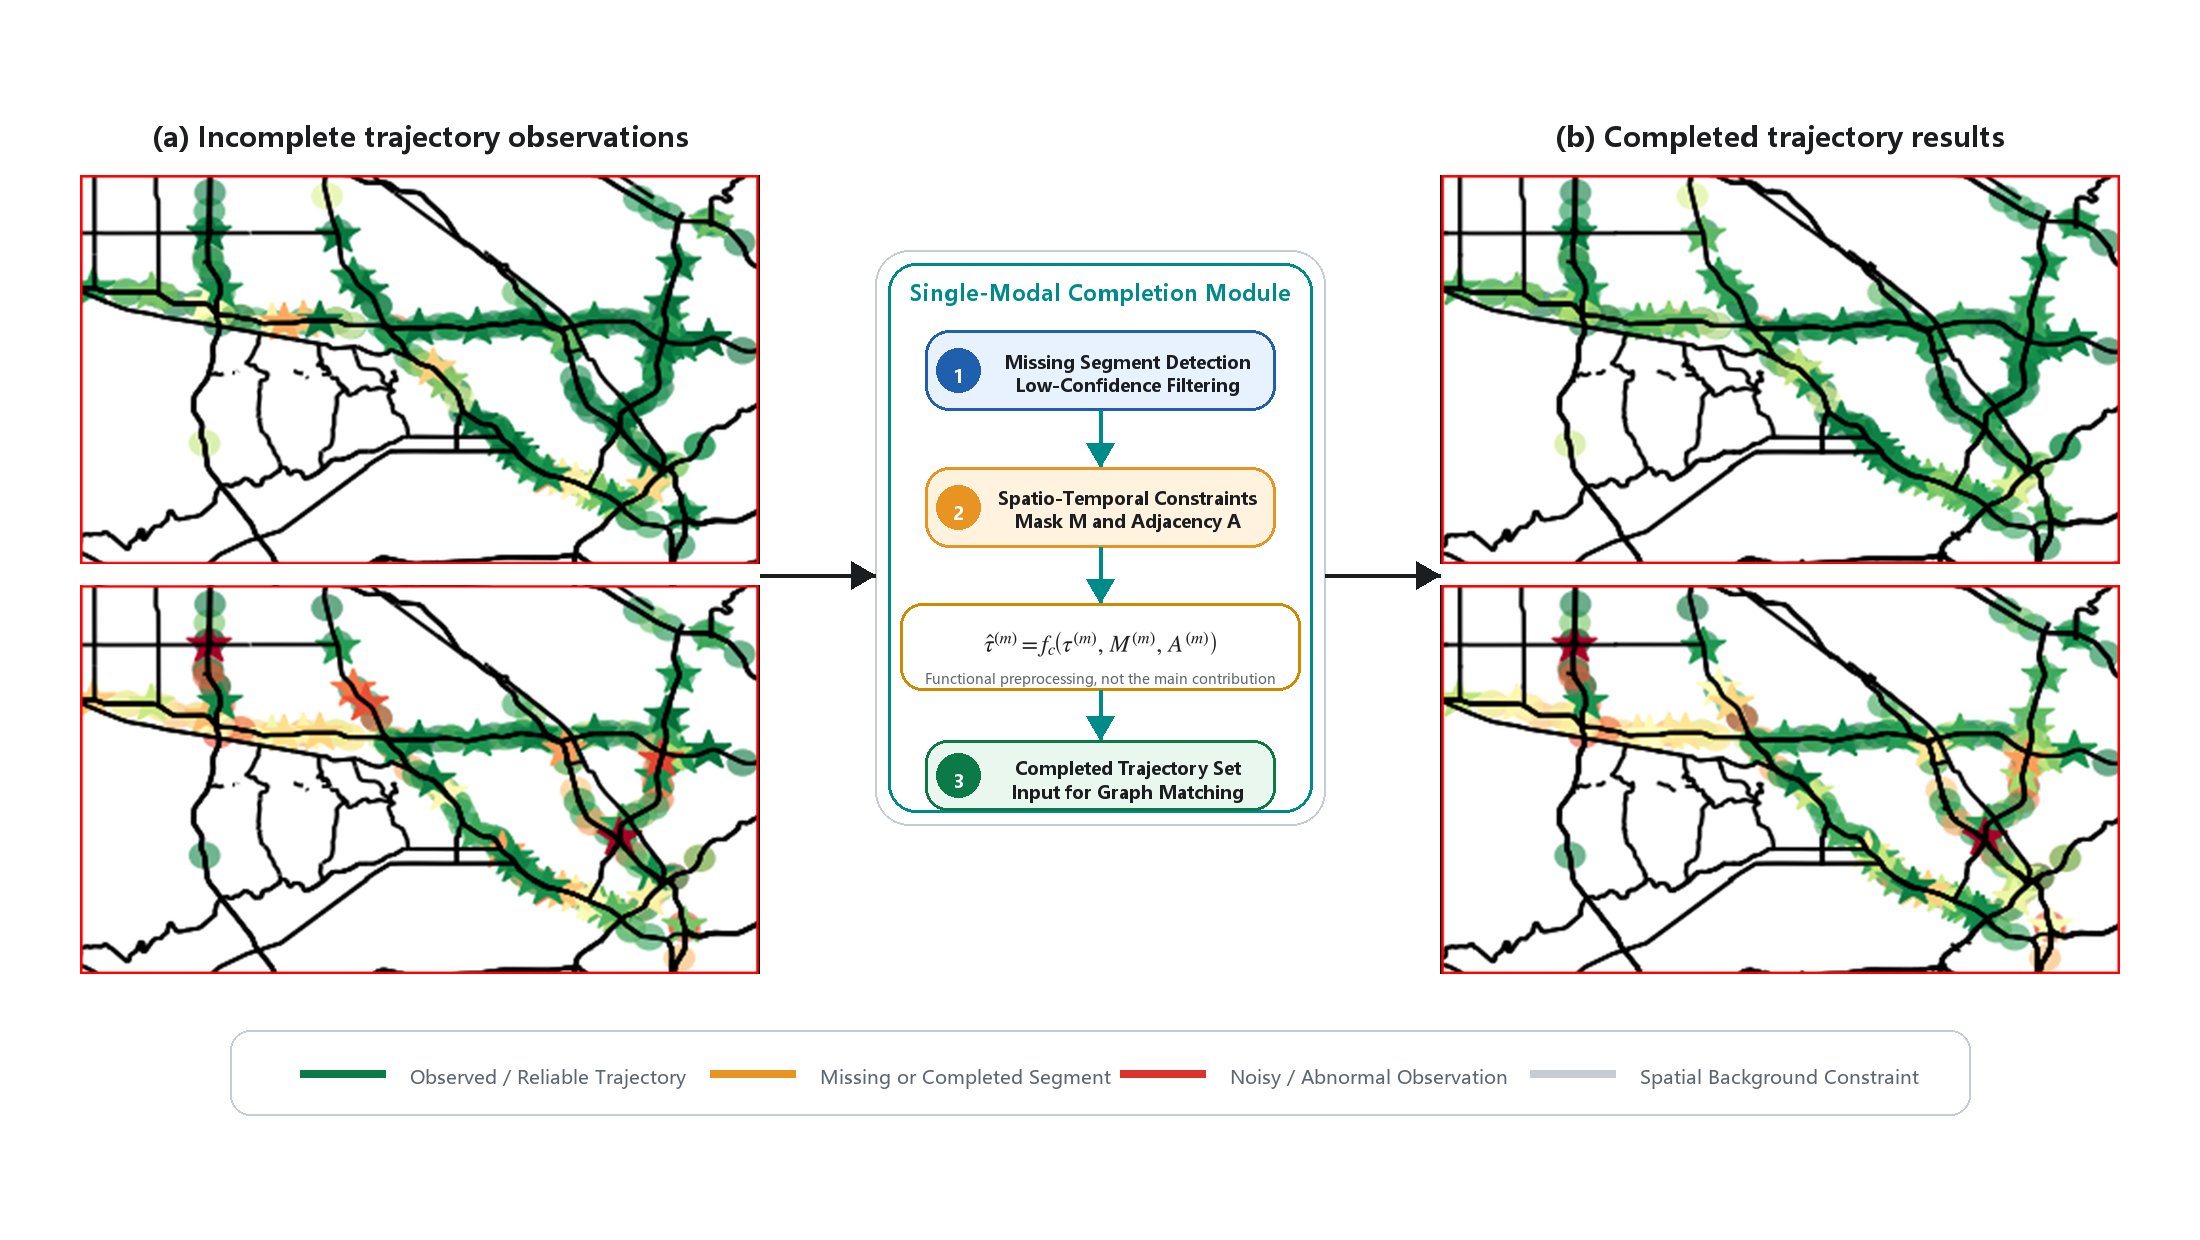
\includegraphics[width=\linewidth]{images/chapter4/trajectory_completion_original_based.png}
  \caption{Functional illustration of single-modal trajectory completion. Incomplete observations are organized through missing-segment detection and spatio-temporal continuity constraints, producing completed trajectory sets that serve as stable inputs for subsequent cross-modal graph matching.}
  \label{fig:chapter4-trajectory-completion}
\end{figure}

Therefore, the completed trajectory set serves as the direct input to the cross-modal registration framework. The notation below starts from \(\mathcal{T}^{(m)}\) and further encodes each completed trajectory into an entity-level descriptor for multi-set matching.

\subsection{Temporal Encoding of Entity Trajectories}
After the upstream completion stage has produced modality-specific entity trajectories, the next step is not to revisit the completion algorithms themselves, but to convert these trajectories into comparable units for cross-modal registration. Although the completed trajectories have a unified format, they still consist of variable-length state sequences. A direct comparison between raw sequences across modalities is inefficient and unstable, especially when the trajectories have different sampling intervals or different attribute dimensions. Therefore, the first task of this chapter is to encode each completed trajectory into a compact embedding that summarizes its temporal dynamics and target-level characteristics.

For each trajectory \(\tau_i^{(m)}\), a temporal encoder \(\Phi_{\mathrm{time}}(\cdot)\) is applied:
\begin{equation}
  h_i^{(m)} = \Phi_{\mathrm{time}}\big(\tau_i^{(m)}\big) \in \mathbb{R}^{d},
\end{equation}
where \(h_i^{(m)}\) is the \(d\)-dimensional entity embedding of the \(i\)-th trajectory in modality \(m\). The encoder may be implemented with a temporal aggregation network, a sequence encoder, or another trajectory modelling backbone. In this thesis, the exact architecture is less important than the role of the encoder: it compresses temporal evolution into a fixed-dimensional representation that can be compared and refined in the later graph matching stage. This step plays a role similar to the feature extraction stage used in feature-based registration pipelines such as PointNet, PointNetLK, DCP, and RPM-Net \cite{qi2017pointnet,aoki2019pointnetlk,wang2019dcp,yew2020rpmnet}.

The temporal embedding is expected to preserve three kinds of information. First, it should encode the motion evolution of the entity, including direction changes, velocity patterns, and temporal continuity. Second, it should retain modality-specific target attributes that remain informative after temporal aggregation. Third, it should be robust to local perturbations, missing states, and moderate observation uncertainty. In this way, the output embedding becomes a stable target-level descriptor rather than a simple average of per-time-step features.

After temporal encoding, each modality-specific entity set can be written as
\begin{equation}
  \mathcal{H}^{(m)} = \{h_1^{(m)},h_2^{(m)},\ldots,h_{N_m}^{(m)}\}.
\end{equation}
These embeddings form the basic node features used in the multi-set graph matching framework. Therefore, the function of Section 4.3 is simply to transform completed trajectories into compact entity representations, which are then refined and aligned in the next section.

\section{Cross-Modal Entity Registration Based on Multi-Set Graph Matching}

\subsection{Problem Formulation of Cross-Modal Entity Registration}
Given one reference modality and multiple source modalities, the goal of cross-modal entity registration is to determine which entities correspond to the same physical target across heterogeneous entity sets. Let the reference entity set be denoted by
\begin{equation}
  \mathcal{R} = \{r_1,r_2,\ldots,r_M\},
\end{equation}
and let the source entity sets be denoted by
\begin{equation}
  \mathcal{S} = \{\mathcal{S}_1,\mathcal{S}_2,\ldots,\mathcal{S}_K\}, \qquad
  \mathcal{S}_k = \{s^k_1,s^k_2,\ldots,s^k_{N_k}\},
\end{equation}
where each \(r_j\) or \(s^k_i\) is represented by the trajectory embedding obtained in Section 4.3.

The registration task is not to estimate a rigid geometric transformation as in classical point-set registration. Instead, it is to infer an entity-level correspondence structure between the source sets and the reference set. Formally, for each source set \(\mathcal{S}_k\), the objective is to estimate a correspondence matrix
\begin{equation}
  \Pi_k \in [0,1]^{N_k \times M},
\end{equation}
where \(\Pi_k(i,j)\) indicates the confidence that source entity \(s^k_i\) and reference entity \(r_j\) belong to the same physical target.

Unlike independent pairwise registration, the present formulation jointly uses all source sets during matching. This is important because different source modalities may provide complementary evidence. One source may preserve clearer temporal regularity, another may preserve more stable spatial structure, and a third may contribute stronger target-level semantics. A multi-set formulation makes it possible to use these complementary cues together instead of aligning every source in isolation.

Therefore, the cross-modal registration problem in this chapter can be summarized as follows: given multiple modality-specific entity sets represented by trajectory embeddings, construct a relational matching framework that refines node features through intra-set and cross-set interaction, evaluates the reliability of cross-modal evidence, and outputs a soft correspondence structure for entity-level alignment.

\begin{figure}[htb]
  \centering
  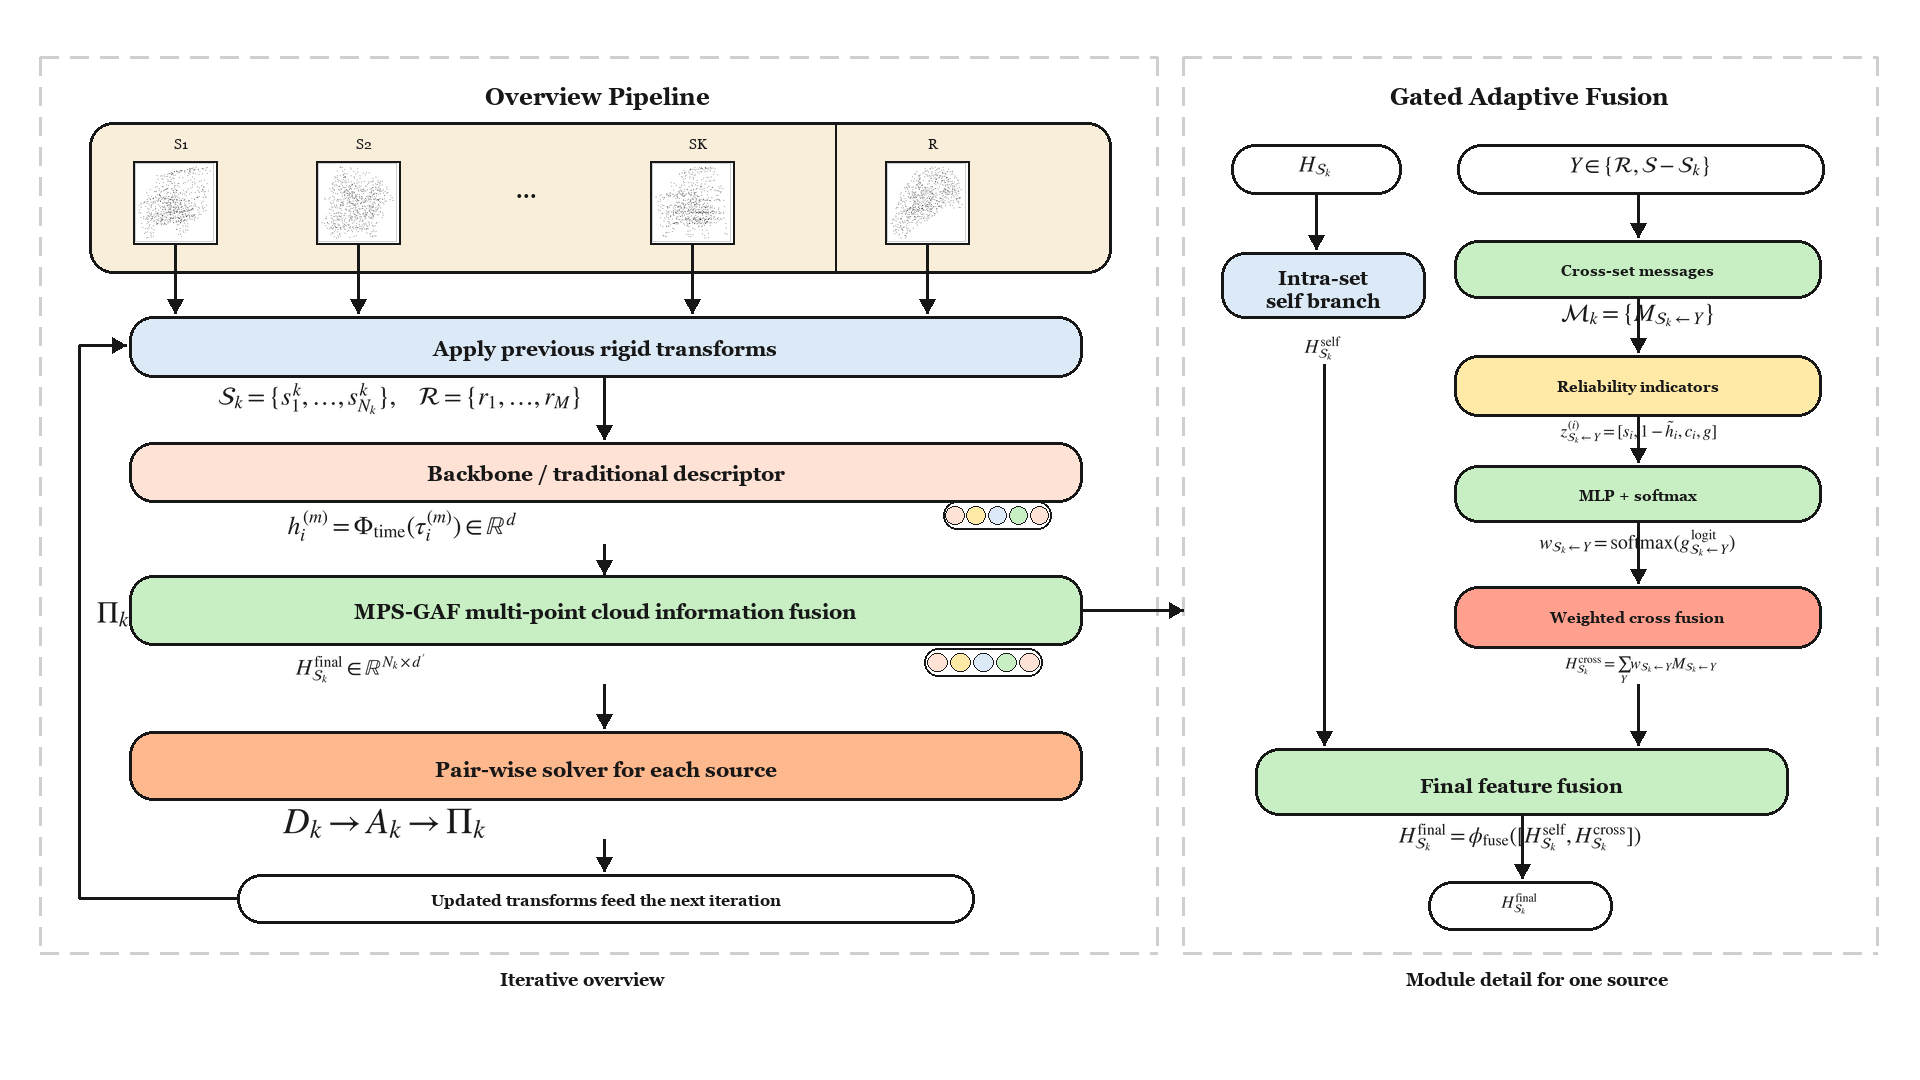
\includegraphics[width=\linewidth]{images/chapter4/multiset_graph_matching_framework.png}
  \caption{Overview of the multi-set graph matching framework. Completed entity trajectories are first encoded into target-level embeddings, then refined through intra-set interaction, cross-set information exchange, and reliability-aware fusion, and finally used to generate soft entity correspondences across modality-specific sets.}
  \label{fig:chapter4-framework}
\end{figure}

\subsection{Intra-Set and Cross-Set Feature Interaction}
The trajectory embeddings obtained in Section 4.3 provide compact target-level descriptors, but they do not yet fully encode the relational structure within each modality or the complementary interaction across modalities. To address this limitation, the proposed framework refines these embeddings in two stages: intra-set structural interaction and cross-set information exchange. The overall design follows the general idea of combining learned descriptors with relation-aware matching rather than relying only on isolated local similarity \cite{yew2020rpmnet,fu2023deepgraphmatching}.

For any entity set \(\mathcal{U}=\{u_1,\ldots,u_n\}\), where each \(u_i \in \mathbb{R}^{d}\), the framework first performs intra-set interaction to preserve modality-internal relational structure. The entity embeddings are projected into a latent interaction space:
\begin{equation}
  T_{\mathcal{U}} = U W_T,
\end{equation}
where \(U \in \mathbb{R}^{n \times d}\) is the stacked embedding matrix and \(W_T \in \mathbb{R}^{d \times d'}\) is a learnable projection. The pairwise similarity matrix inside the set is then computed as
\begin{equation}
  S^{\mathrm{intra}}_{\mathcal{U}} = T_{\mathcal{U}}T_{\mathcal{U}}^{\top}.
\end{equation}
After row-wise normalization, the resulting relation weights describe how strongly each entity should aggregate information from the other entities in the same set. This process helps the embedding of one entity absorb contextual information from neighboring entities and from the local group structure in the same modality.

The intra-set refined feature can therefore be written as
\begin{equation}
  H^{\mathrm{self}}_{\mathcal{U}} =
  \operatorname{softmax}\!\left(\frac{S^{\mathrm{intra}}_{\mathcal{U}}}{\tau}\right) U W_A + U W_S,
\end{equation}
where \(W_A\) and \(W_S\) are learnable mappings and \(\tau\) is a temperature parameter. The first term propagates structural information across related entities, while the second term preserves the original target identity branch.

After intra-set refinement, the framework performs cross-set interaction between different modality-specific entity sets. Let \(\mathcal{X}\) and \(\mathcal{Y}\) denote two distinct entity sets. Their embeddings are projected into a shared latent space:
\begin{equation}
  T^{\mathrm{cross}}_X = XW_X, \qquad T^{\mathrm{cross}}_Y = YW_Y,
\end{equation}
where \(X\) and \(Y\) are the stacked entity embedding matrices. The cross-set similarity matrix is then defined as
\begin{equation}
  S_{X \leftarrow Y}^{\mathrm{cross}} = T^{\mathrm{cross}}_X \big(T^{\mathrm{cross}}_Y\big)^\top.
\end{equation}
After normalization, the matrix gives the relevance of every entity in \(\mathcal{X}\) to all entities in \(\mathcal{Y}\). Based on this relation, a message from \(\mathcal{Y}\) to \(\mathcal{X}\) is aggregated:
\begin{equation}
  M_{X \leftarrow Y} =
  \operatorname{softmax}\!\left(\frac{S_{X \leftarrow Y}^{\mathrm{cross}}}{\tau}\right) YW_C.
\end{equation}

This design allows each entity set to receive complementary evidence from the reference set and from other source sets. In the present cross-modal scenario, such interaction is useful because one modality may compensate for another when local target evidence is weak, spatial precision is unstable, or a subset of entities is incompletely observed. Therefore, the role of this subsection is to refine the trajectory embeddings into relation-aware entity features before reliability-aware fusion is applied.

\subsection{Reliability-Aware Gated Fusion for Cross-Modal Matching}
If the messages collected from different entity sets are directly averaged, noisy or low-quality modality evidence may be propagated to the entire registration process. This problem is particularly serious in the present thesis setting because the sensing modalities do not have identical reliability. Their localization precision, observation density, and feature discriminability may vary significantly across scenes. Therefore, the cross-set messages should be fused adaptively rather than treated equally.

For a source entity set \(\mathcal{S}_k\), suppose that the framework has collected a group of incoming cross-set messages
\begin{equation}
  \mathcal{M}_k = \{M_{\mathcal{S}_k \leftarrow Y} \mid Y \in \{\mathcal{R}, \mathcal{S}\setminus \mathcal{S}_k\}\}.
\end{equation}
The objective of gated fusion is to determine how much information should be accepted from each incoming set \(Y\). To do this, the framework computes a group of reliability indicators from the cross-set similarity or correspondence distributions.

The first indicator is matching sharpness, which measures whether the relation distribution is concentrated around a few candidate correspondences. The second indicator is entropy, which measures uncertainty in the matching distribution. The third indicator is bidirectional consistency, which measures whether the relation from set \(X\) to set \(Y\) is supported by the reverse relation from \(Y\) back to \(X\). The fourth indicator is a global similarity measure between the two sets, which reflects their coarse semantic compatibility. Together, these indicators describe whether the message from \(Y\) should be trusted when refining the source set \(\mathcal{S}_k\).

More specifically, for the relation matrix \(E_{X \leftarrow Y}\), the sharpness of the \(i\)-th source entity is defined as
\begin{equation}
  s_i = \max_j E_{X \leftarrow Y}(i,j),
\end{equation}
the entropy is defined as
\begin{equation}
  \tilde{h}_i
  =
  - \frac{1}{\log |Y|}
  \sum_j E_{X \leftarrow Y}(i,j)\log E_{X \leftarrow Y}(i,j),
\end{equation}
and the bidirectional consistency is defined as
\begin{equation}
  c_i = \sum_j E_{X \leftarrow Y}(i,j) E_{Y \leftarrow X}(j,i).
\end{equation}
In addition, the global similarity score is written as
\begin{equation}
  g(X,Y) = \frac{\langle \bar{x},\bar{y} \rangle}{\|\bar{x}\|\,\|\bar{y}\|},
\end{equation}
where \(\bar{x}\) and \(\bar{y}\) denote the mean embeddings of the two sets. Since \(g(X,Y)\) is a set-level scalar while \(s_i\), \(\tilde{h}_i\), and \(c_i\) are entity-level indicators, the scalar value is broadcast to every entity in the source set before concatenation. These quantities allow the gate to jointly consider local matching confidence and coarse set-level compatibility.

For every incoming set \(Y\), the reliability vector is written as
\begin{equation}
  z_{\mathcal{S}_k \leftarrow Y}^{(i)}
  =
  \operatorname{Concat}[s_i,\ 1-\tilde{h}_i,\ c_i,\ g(X,Y)],
\end{equation}
where \(s_i\) denotes sharpness, \(\tilde{h}_i\) denotes normalized entropy, \(c_i\) denotes bidirectional consistency, and \(g(X,Y)\) denotes global similarity. The reliability vector is fed to a lightweight gating function \(G(\cdot)\):
\begin{equation}
  g_{\mathcal{S}_k \leftarrow Y}^{\mathrm{logit}} = \frac{1}{|\mathcal{S}_k|}\sum_i G\big(z_{\mathcal{S}_k \leftarrow Y}^{(i)}\big).
\end{equation}
The normalized fusion weight is then obtained by competitive softmax:
\begin{equation}
  w_{\mathcal{S}_k \leftarrow Y}
  =
  \frac{
    \exp\big(g_{\mathcal{S}_k \leftarrow Y}^{\mathrm{logit}}\big)
  }{
    \sum_{Y'} \exp\big(g_{\mathcal{S}_k \leftarrow Y'}^{\mathrm{logit}}\big)
  }.
\end{equation}

Based on these weights, the final cross-set feature of \(\mathcal{S}_k\) is written as
\begin{equation}
  H^{\mathrm{cross}}_{\mathcal{S}_k}
  =
  \sum_Y
  w_{\mathcal{S}_k \leftarrow Y} M_{\mathcal{S}_k \leftarrow Y}.
\end{equation}
This design makes the matching framework reliability-aware in two senses. First, high-confidence correspondence patterns contribute more strongly to the final feature. Second, unreliable modality evidence is suppressed instead of being injected into the registration stage without control. This is especially important in multimodal target fusion because the framework must tolerate modality-dependent localization errors and partial observation defects.

Finally, the self feature and the cross-set feature are fused into the refined registration feature:
\begin{equation}
  H^{\mathrm{final}}_{\mathcal{S}_k}
  =
  \phi_{\mathrm{fuse}}
  \big(
    \operatorname{Concat}[H^{\mathrm{self}}_{\mathcal{S}_k},\, H^{\mathrm{cross}}_{\mathcal{S}_k}]
  \big),
\end{equation}
where \(\phi_{\mathrm{fuse}}(\cdot)\) is a lightweight fusion mapping. The same operation is applied to the reference set. The output features then serve as the direct input to soft correspondence estimation.

\subsection{Soft Correspondence and Entity-Level Registration Output}
After relation-aware feature refinement, entity-level correspondences are estimated through a soft assignment mechanism. For each source set \(\mathcal{S}_k\) and the reference set \(\mathcal{R}\), the pairwise feature distance matrix is first computed:
\begin{equation}
  D_k(i,j)
  =
  \left\lVert
    H^{\mathrm{final}}_{\mathcal{S}_k}(i,:)
    -
    H^{\mathrm{final}}_{\mathcal{R}}(j,:)
  \right\rVert_2^2 .
\end{equation}
The distance matrix is then converted into an affinity matrix
\begin{equation}
  A_k(i,j) = -\beta_k \big(D_k(i,j)-\alpha_k\big),
\end{equation}
where \(\beta_k\) and \(\alpha_k\) control the scale and offset of the matching affinity.

To avoid forcing every entity into a hard one-to-one decision too early, the framework uses soft assignment and obtains a correspondence matrix
\begin{equation}
  \Pi_k = \operatorname{Sinkhorn}\big(\exp(A_k)\big).
\end{equation}
Here, \(\Pi_k(i,j)\) can be interpreted as the confidence that source entity \(s^k_i\) corresponds to reference entity \(r_j\). The soft assignment is more suitable than immediate hard matching because cross-modal alignment may remain ambiguous when observations are partially missing, local structures are similar, or modality gaps are strong. This formulation is consistent with the differentiable correspondence estimation strategy adopted in robust point matching pipelines such as RPM-Net \cite{yew2020rpmnet}.

The entity-level registration result is then derived from the soft correspondence structure. For each source entity, let
\begin{equation}
  j_i^{\ast} = \arg\max_j \Pi_k(i,j), \qquad
  p_i^{\ast} = \max_j \Pi_k(i,j).
\end{equation}
If \(p_i^{\ast} \ge \eta_{\mathrm{match}}\), the source entity is assigned to the reference identity \(r_{j_i^{\ast}}\). Otherwise, it is treated as an unmatched target:
\begin{equation}
  \mathcal{U}_k = \{s_i^k \mid p_i^{\ast} < \eta_{\mathrm{match}}\}.
\end{equation}
The unmatched set \(\mathcal{U}_k\) collects new, temporarily missing, or low-confidence entities that should not be forced into the current fusion groups. In this way, the output of registration is not limited to a closed-set one-to-one assignment, but remains compatible with realistic multimodal sensing conditions.

In implementation, the training objective of the registration stage follows the adopted underlying registration module rather than being redesigned independently in this chapter. More specifically, the entity-level formulation inherits the same correspondence-driven supervision and inlier regularization strategy used by the base matching framework \cite{wang2019dcp,yew2020rpmnet}. The emphasis of the present chapter is therefore on adapting the input representation, relation modeling, and output interpretation of the registration module to the multimodal entity-alignment setting.

Let \(\Gamma_k\) denote the final matched correspondence set between source set \(\mathcal{S}_k\) and reference set \(\mathcal{R}\). The registration output over all source modalities is written as
\begin{equation}
  \Gamma = \{\Gamma_1,\Gamma_2,\ldots,\Gamma_K\}, \qquad
  \Gamma_k = \{(s_i^k,r_{j_i^{\ast}})\mid p_i^{\ast}\ge \eta_{\mathrm{match}}\}.
\end{equation}
This output establishes the identity relationship required by multimodal target fusion, while \(\mathcal{U}_k\) preserves entities that should remain unmatched in the current step. Once the reliable entities have been aligned across modalities, the system can merge their trajectories and attributes into a unified target-level representation.

\section{Fusion Result Representation}

\subsection{Entity-Level Fusion Result Generation}
After the cross-modal correspondence structure \(\Gamma\) has been obtained, the next step is to convert registration results into entity-level fusion outputs. Let \(e_j\) denote the \(j\)-th fused entity in the unified representation space. All source entities that are assigned or strongly matched to the same reference identity are collected into one fusion group:
\begin{equation}
  \mathcal{C}_j = \{r_j\} \cup \{s^k_i \mid (s^k_i,r_j) \in \Gamma_k\}.
\end{equation}
For notational convenience, let the corresponding source-index set be
\begin{equation}
  \mathcal{I}_j = \{(k,i)\mid s_i^k \in \mathcal{C}_j\}.
\end{equation}

The trajectory information, modality-specific attributes, and correspondence confidence inside each group are then aggregated to generate the fused entity result. In generic form, the fused representation of entity \(e_j\) is written as
\begin{equation}
  e_j = \{T_j,\ F_j,\ C_j\},
\end{equation}
where \(T_j\) denotes the fused trajectory description, \(F_j\) denotes the fused multi-modal attribute representation, and \(C_j\) denotes confidence information derived from the registration stage.

For every member \(s_i^k \in \mathcal{C}_j\), let the registration-supported fusion score be
\begin{equation}
  \rho_{j}^{(k,i)} = \Pi_k(i,j)\,\bar{c}_i^{(k)},
\end{equation}
where \(\bar{c}_i^{(k)}\) denotes the average observation confidence of the \(i\)-th trajectory in modality \(k\). The normalized fusion weight is then written as
\begin{equation}
  \omega_{j}^{(k,i)} =
  \frac{\rho_{j}^{(k,i)}}{\sum_{(m,n)\in \mathcal{I}_j}\rho_{j}^{(m,n)}}.
\end{equation}
Based on these weights, the fused trajectory component at time index \(t\) is defined as
\begin{equation}
  T_j(t) =
  \frac{
    \sum_{(k,i)\in \mathcal{I}_j}
    \omega_{j}^{(k,i)} \mu_{i,t}^{(k)} p_{i,t}^{(k)}
  }{
    \sum_{(k,i)\in \mathcal{I}_j}
    \omega_{j}^{(k,i)} \mu_{i,t}^{(k)}
  },
\end{equation}
where \(\mu_{i,t}^{(k)}\in\{0,1\}\) is the validity mask defined in Chapter 2. In this way, missing observations do not force invalid trajectory values into the fused result.

The fused multi-modal attribute vector is obtained by weighted aggregation of modality-specific trajectory descriptors:
\begin{equation}
  F_j =
  \sum_{(k,i)\in \mathcal{I}_j}
  \omega_{j}^{(k,i)} \bar{f}_{i}^{(k)},
\end{equation}
where \(\bar{f}_{i}^{(k)}\) denotes the temporally aggregated attribute representation of the matched trajectory. Finally, the fusion confidence is computed as
\begin{equation}
  C_j =
  \sum_{(k,i)\in \mathcal{I}_j}
  \omega_{j}^{(k,i)} \rho_{j}^{(k,i)}.
\end{equation}
The quantity \(C_j\) jointly reflects matching confidence and trajectory quality, so that fused entities derived from weak correspondences or unreliable observations can be identified in later behavior analysis.

The trajectory component \(T_j\) therefore summarizes the motion of the entity after cross-modal alignment, while the feature component \(F_j\) preserves the modality-specific attributes contributed by optical, electromagnetic, SAR, and other sources. In practice, this means that the fused entity no longer belongs to one single modality, but becomes a target-centered object with cross-source information support.

Therefore, the registration stage and the fusion stage have different functions. Registration determines which entities correspond across modalities, while fusion determines how their information should be summarized into a single entity description. This distinction is important because the thesis does not equate correspondence estimation with full target fusion; instead, fusion is explicitly defined as a post-registration aggregation step.

\subsection{Unified Entity Representation for Behavior Analysis}
The final objective of this chapter is not merely to produce correspondence matrices, but to provide structured inputs for high-level behavior analysis. For that reason, the fused entity representation must remain interpretable and suitable for downstream temporal and group-level reasoning.

In this thesis, each fused entity is represented as a structured target record containing at least three categories of information: a trajectory component, a multi-modal attribute component, and a confidence component. The trajectory component supports later group motion analysis, spatiotemporal consistency modeling, and anomaly detection. The attribute component preserves complementary evidence that may help distinguish similar motion patterns under different sensing conditions. The confidence component records the reliability of the underlying cross-modal alignment and can later be used to control the influence of uncertain entities in behavior analysis.

Let the final fused entity set be denoted by
\begin{equation}
  \mathcal{F} = \{e_1,e_2,\ldots,e_{N_f}\},
\end{equation}
where \(N_f\) is the number of registered entities after cross-modal fusion. The set \(\mathcal{F}\) serves as the direct input to Chapter 5. In this way, the present chapter completes the transition from modality-specific trajectory sets to a unified entity space, which is the necessary basis for subsequent group behavior modeling and situation understanding.

\section{Experiments and Result Analysis}

\subsection{Experimental Setup and Evaluation Metrics}
The experiments in this chapter are designed to evaluate whether the proposed trajectory-encoding and multi-set graph matching framework can produce robust registration under both standard and degraded observation conditions. Since the core registration module is developed from an existing multi-set matching pipeline, the present experiments first validate its behavior in a controlled setting and then use the results to support its integration into the multimodal target fusion framework.

The experimental data are constructed on ModelNet40 \cite{wu2015shapenets}. Following the standard preprocessing protocol of the multi-set registration module, 2,048 points are uniformly sampled from each mesh and normalized to a unit sphere. During both training and testing, each example contains one target set and \(N\) source sets. Each source set is perturbed by a random rigid transformation, while the target set remains fixed. In the multi-set setting, the source sets are independently sampled for the same target object so that the registration method must jointly exploit complementary evidence across multiple views.

Although these experiments are performed on point-set data rather than directly on the multimodal target trajectories in the final system, they provide a controlled validation of the graph matching module used in this thesis. Their purpose is to verify whether the multi-set interaction and reliability-aware fusion design remain effective under clean, noisy, and incomplete conditions before the method is embedded into the entity-level registration stage of the target fusion framework.

The bridge between the benchmark setting and the thesis task lies in the matching mechanism rather than in the physical meaning of the raw data. In the benchmark experiments, each point set acts as a structured node set whose internal relations and cross-set correspondences must be inferred jointly. In the target-fusion system, the same role is played by modality-specific entity sets after temporal encoding, where each node corresponds to an entity trajectory or target state rather than a geometric point. Under this view, point-set correspondence matrices correspond to cross-modal entity association matrices, jitter and perturbation correspond to localization errors and attribute noise, and cropping or partial overlap correspond to missed detections, occlusion, and incomplete target observations. Therefore, the ModelNet40 experiments do not claim to reproduce the full multimodal fusion pipeline directly; instead, they provide controlled evidence that the underlying graph matching and reliability-aware registration mechanism is suitable for the entity-level alignment problem considered in this chapter.

Five metrics are used to evaluate registration quality, following \cite{yew2020rpmnet,wang2019dcp}. Two isotropic metrics are the Mean Isotropic Error of Rotation, denoted as \(\mathrm{MIE(R)}\), and the Mean Isotropic Error of Translation, denoted as \(\mathrm{MIE(t)}\). Two anisotropic metrics are the Mean Absolute Error of Rotation, denoted as \(\mathrm{MAE(R)}\), and the Mean Absolute Error of Translation, denoted as \(\mathrm{MAE(t)}\). In addition, the Corrected Chamfer Distance, denoted as \(\mathrm{CCD}\), measures the geometric discrepancy after registration while suppressing far outliers. In the present chapter, these metrics are used to evaluate the quality and robustness of the underlying registration module that supports cross-modal entity alignment.

The compared methods include classical registration baselines, deep pairwise registration methods, and representative multi-set registration methods, including ICP \cite{besl1992icp}, FGR \cite{zhou2016fgr}, MAC \cite{zhang2023mac}, PointNetLK \cite{aoki2019pointnetlk}, DCP \cite{wang2019dcp}, RPM-Net \cite{yew2020rpmnet}, JRMPC \cite{evangelidis2018joint}, and EMPMR \cite{zhu2020multiviewem}. In particular, the registration framework is implemented on top of RPM-Net \cite{yew2020rpmnet} so that the improvement introduced by multi-set interaction and gated fusion can be evaluated against a strong pairwise backbone. This comparison directly supports the main claim of this chapter: entity-level registration becomes more robust when multiple sets are jointly modeled instead of aligned independently. Additional dataset-wise benchmark results are reported in Appendix~\ref{chap:appendix-registration-benchmark}; they are kept outside the main chapter so that the main text can focus on the controlled ModelNet40 analysis.

\subsection{Performance Under Standard Conditions}
Under standard observation conditions, the purpose of the experiment is to examine whether the proposed framework can accurately align multiple source entity sets to the reference set when the observations are relatively complete and the noise level is moderate. In this setting, the main challenge is not severe corruption, but the need to exploit complementary cross-set information better than independent pairwise matching.

The expected behavior of the proposed framework is as follows. First, the temporal encoder provides compact entity embeddings that already preserve meaningful target evolution patterns. Second, intra-set interaction improves these embeddings by injecting structural context from the same modality. Third, cross-set interaction allows different source sets to exchange complementary evidence before correspondence estimation. As a result, the final soft correspondence matrices should be more stable and more discriminative than those obtained from direct pairwise matching.

Quantitatively, the results confirm this expectation. As shown in Table~\ref{tab:chapter4-clean}, the proposed multi-set graph matching framework achieves the best performance on all five metrics under clean conditions, with consistent improvements over the pairwise backbone RPM-Net. Although the gap is not large in this relatively easy setting, the result demonstrates that the explicit use of intra-set structure and cross-set complementarity can still reduce both rotation and translation errors.

\begin{table}[htb]
  \centering
  \caption{Performance under standard conditions. Bold and underline denote the best and second-best results.}
  \label{tab:chapter4-clean}
  \begin{tabular}{lccccc}
    \toprule
    Method & MIE(R) & MIE(t) & MAE(R) & MAE(t) & CCD \\
    \midrule
    ICP & 19.776 & 0.1370 & 11.710 & 0.0792 & 0.00358 \\
    FGR & 10.235 & 0.0603 & 6.506 & 0.0348 & 0.000869 \\
    MAC & 8.340 & 0.0539 & 6.774 & 0.0311 & 0.00110 \\
    PointNetLK & 8.842 & 0.0631 & 5.375 & 0.0323 & 0.00245 \\
    DCP & 6.733 & 0.0615 & 4.221 & 0.0313 & 0.00228 \\
    JRMPC & 3.578 & 0.0247 & 1.903 & 0.0142 & 0.00364 \\
    EMPMR & 20.141 & 0.1420 & 11.972 & 0.0819 & 0.00374 \\
    RPM-Net & \underline{0.468} & \underline{0.00347} & \underline{0.305} & \underline{0.00200} & \underline{0.0000496} \\
    RPM-Net + MPS-GAF & \textbf{0.465} & \textbf{0.00342} & \textbf{0.296} & \textbf{0.00198} & \textbf{0.0000485} \\
    \bottomrule
  \end{tabular}
\end{table}

The qualitative comparison in Fig.~\ref{fig:chapter4-clean} further shows that the jointly modeled source sets can be aligned more coherently to the target set. This observation is consistent with the role assigned to the method in this thesis: before the system aggregates information across modalities, it must first produce a stable correspondence structure, and the result under standard conditions verifies that the proposed framework is capable of doing so.

\begin{figure}[htb]
  \centering
  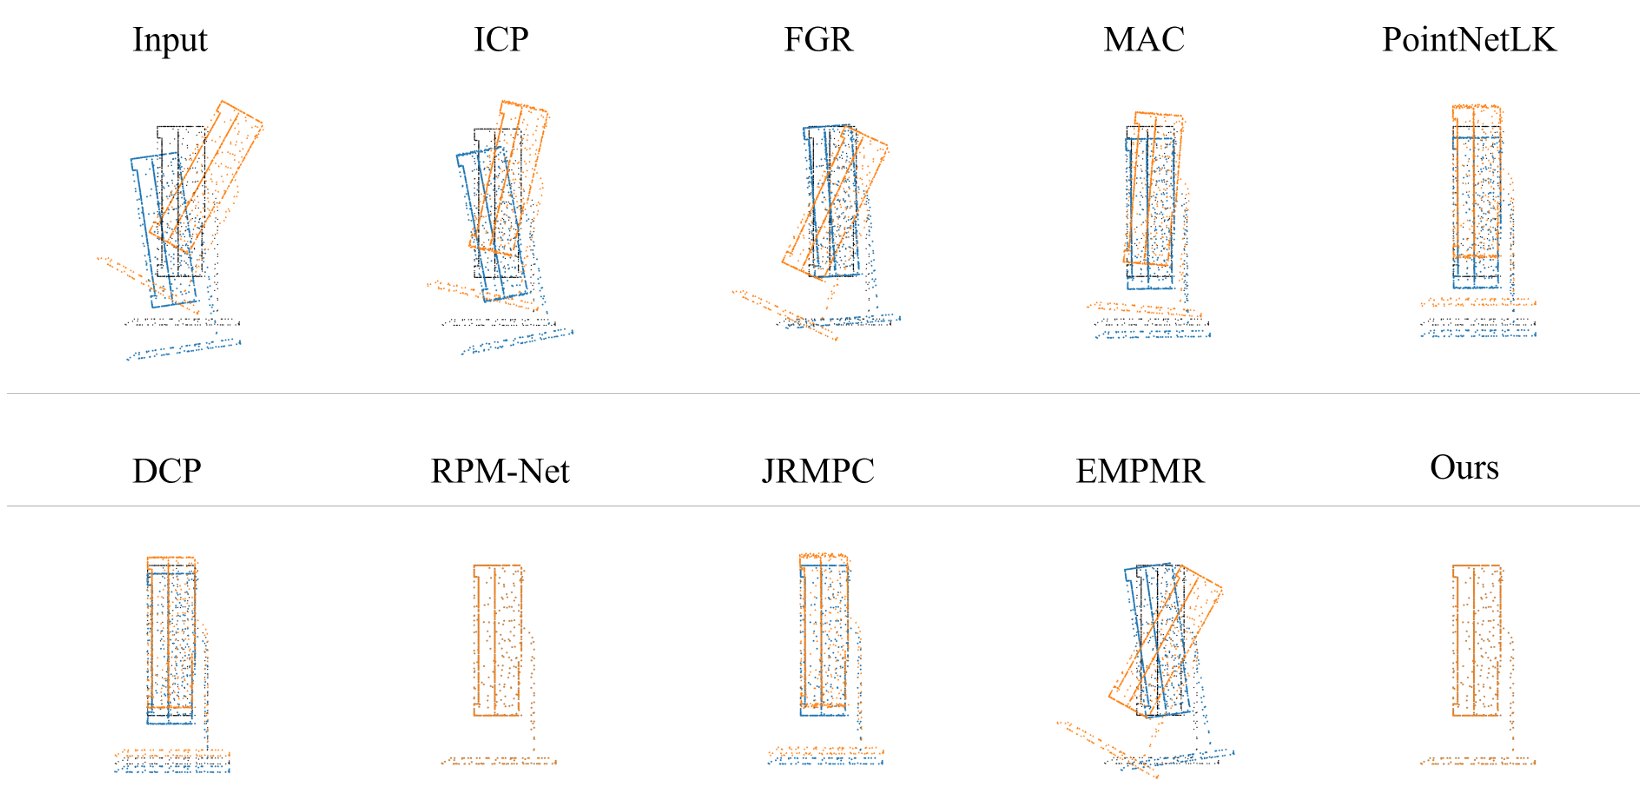
\includegraphics[width=\linewidth]{images/chapter4/registration_standard_conditions.png}
  \caption{Qualitative registration results under standard conditions. Black denotes the target set, while orange and blue denote two source sets.}
  \label{fig:chapter4-clean}
\end{figure}

\subsection{Performance Under Noisy or Incomplete Observations}
The more important test for multimodal target fusion lies in degraded conditions, where the observations are noisy, incomplete, or only partially available. This setting is closely related to real deployment because different sensing modalities rarely provide equally clean and complete target observations. In such cases, local entity descriptors may become ambiguous, and direct pairwise matching may be strongly affected by missing trajectories or unreliable spatial evidence.

The proposed framework addresses this difficulty in two ways. First, multi-set interaction allows one source set to benefit from complementary evidence in the others, reducing the risk that a single weak set dominates the registration result. Second, the reliability-aware gated fusion module explicitly down-weights low-confidence or conflicting incoming messages. Therefore, when observations are noisy or partially missing, the framework is expected to remain more stable than methods that simply average all cross-set information or match one source to the reference independently.

Under noisy conditions, random jitter is injected into both source sets and the target set. The quantitative results in Table~\ref{tab:chapter4-noise} show that the proposed framework still achieves the best performance on all five metrics. Relative to RPM-Net, the improvements are especially visible in the rotation and translation errors, indicating that the interaction modules and gated fusion improve stability under perturbation.

\begin{table}[htb]
  \centering
  \caption{Performance under noisy conditions. Bold and underline denote the best and second-best results.}
  \label{tab:chapter4-noise}
  \begin{tabular}{lccccc}
    \toprule
    Method & MIE(R) & MIE(t) & MAE(R) & MAE(t) & CCD \\
    \midrule
    ICP & 19.956 & 0.1360 & 11.772 & 0.0789 & 0.00320 \\
    FGR & 21.391 & 0.1630 & 13.076 & 0.0943 & 0.00771 \\
    MAC & 8.272 & 0.0572 & 6.234 & 0.0330 & 0.00123 \\
    PointNetLK & 8.842 & 0.0731 & 5.375 & 0.0423 & 0.00345 \\
    DCP & 8.733 & 0.0715 & 5.221 & 0.0413 & 0.00328 \\
    JRMPC & 3.761 & 0.0269 & 2.860 & 0.0155 & 0.00408 \\
    EMPMR & 20.219 & 0.1410 & 11.947 & 0.0817 & 0.00349 \\
    RPM-Net & \underline{1.955} & \underline{0.0137} & \underline{1.159} & \underline{0.00795} & \underline{0.000641} \\
    RPM-Net + MPS-GAF & \textbf{1.634} & \textbf{0.0128} & \textbf{1.016} & \textbf{0.00659} & \textbf{0.000624} \\
    \bottomrule
  \end{tabular}
\end{table}

The qualitative result in Fig.~\ref{fig:chapter4-noise} illustrates the same tendency. Even after perturbation, the multi-set framework produces a more coherent alignment than the pairwise strategy because it can integrate complementary evidence from multiple source sets rather than relying on one noisy matching path alone.

\begin{figure}[htb]
  \centering
  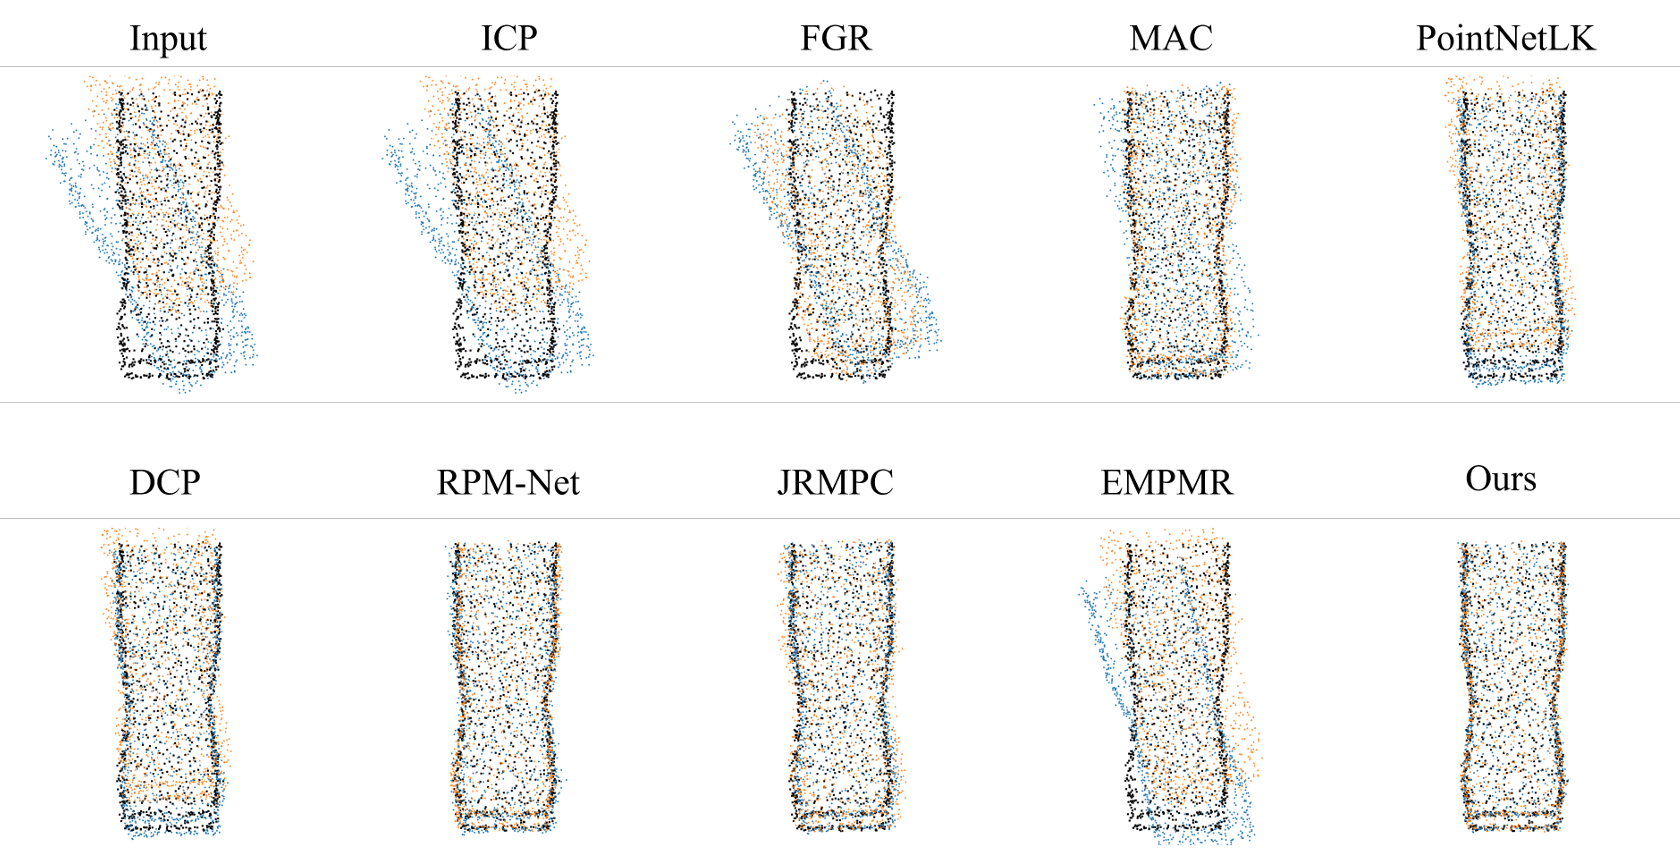
\includegraphics[width=\linewidth]{images/chapter4/registration_noisy_conditions.png}
  \caption{Qualitative registration results under noisy conditions. Black denotes the target set, while orange and blue denote two source sets.}
  \label{fig:chapter4-noise}
\end{figure}

The experiments further evaluate incomplete and partially observed conditions by cropping each set with a randomly oriented halfspace and combining the result with perturbation. This setting is especially relevant to the present thesis, because multimodal target observations are often spatially incomplete or only partially visible. As shown in Table~\ref{tab:chapter4-obstructed}, the proposed multi-set framework again outperforms all baselines under partial visibility.

\begin{table}[htb]
  \centering
  \caption{Performance under noisy and incomplete observations. Bold and underline denote the best and second-best results.}
  \label{tab:chapter4-obstructed}
  \begin{tabular}{lccccc}
    \toprule
    Method & MIE(R) & MIE(t) & MAE(R) & MAE(t) & CCD \\
    \midrule
    ICP & 38.195 & 0.3450 & 22.739 & 0.1990 & 0.0162 \\
    FGR & 48.141 & 0.3930 & 31.568 & 0.2270 & 0.0281 \\
    MAC & 9.409 & 0.0707 & 6.559 & 0.0408 & 0.0184 \\
    PointNetLK & 13.410 & 0.1650 & 8.803 & 0.0914 & 0.00817 \\
    DCP & 12.734 & 0.1500 & 8.094 & 0.0868 & 0.00773 \\
    JRMPC & 4.245 & 0.0418 & 2.363 & 0.0241 & 0.00503 \\
    EMPMR & 37.232 & 0.3370 & 22.058 & 0.1940 & 0.0153 \\
    RPM-Net & \underline{3.228} & \underline{0.0332} & \underline{2.137} & \underline{0.0193} & \underline{0.000852} \\
    RPM-Net + MPS-GAF & \textbf{2.956} & \textbf{0.0321} & \textbf{1.955} & \textbf{0.0172} & \textbf{0.000723} \\
    \bottomrule
  \end{tabular}
\end{table}

The qualitative case in Fig.~\ref{fig:chapter4-crop} shows why the gain is larger in this more difficult setting. The adaptive gate fusion mechanism suppresses inconsistent or weak source evidence and preserves cross-set support from the more reliable local structures. This characteristic is precisely the reason why the method is useful for multimodal target fusion, where incomplete observations are common.

\begin{figure}[htb]
  \centering
  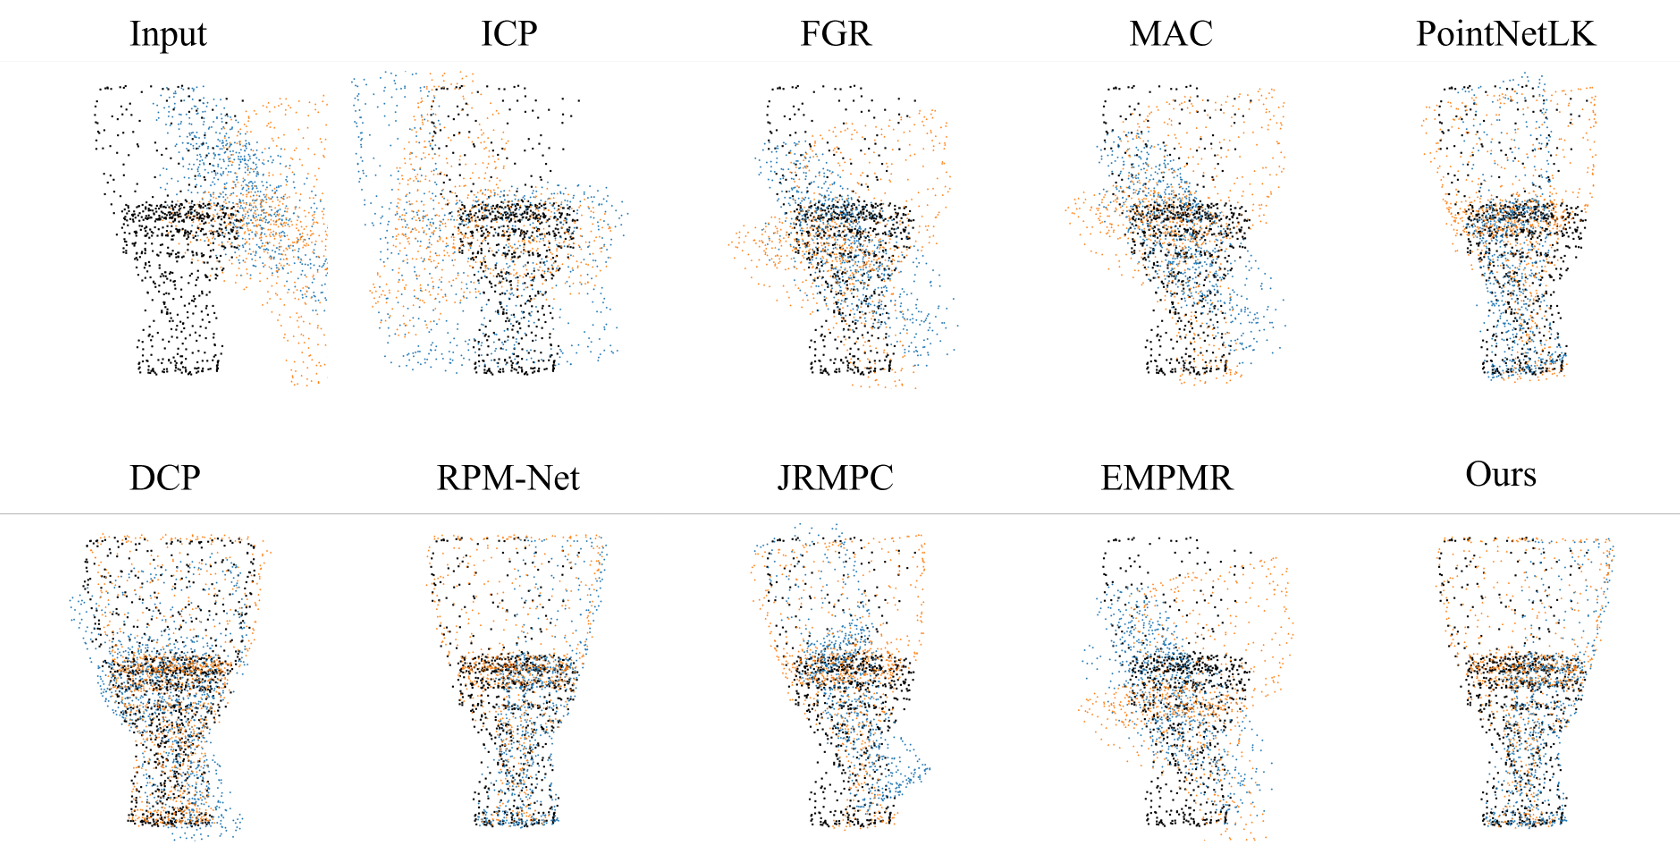
\includegraphics[width=\linewidth]{images/chapter4/registration_noisy_incomplete_conditions.png}
  \caption{Qualitative registration results under noisy and incomplete observations. Black denotes the target set, while orange and blue denote two source sets.}
  \label{fig:chapter4-crop}
\end{figure}

\subsection{Discussion of Cross-Modal Registration Results}
The experimental results should be interpreted from the perspective of the proposed registration mechanism rather than as isolated numerical gains. When the framework performs well, the improvement is mainly due to three factors. First, trajectory encoding converts variable-length entity observations into stable embeddings, making cross-modal comparison more feasible. Second, intra-set and cross-set interaction inject relation-aware context into the matching process, which reduces the ambiguity of local entity features. Third, reliability-aware fusion prevents low-quality source evidence from overwhelming the final registration decision.

From a multimodal target fusion viewpoint, the significance of these results is that entity registration becomes more robust when it is treated as a structured multi-set problem instead of a collection of independent pairwise tasks. This is consistent with the practical intuition that the same physical target should be supported by multiple forms of evidence across modalities, and that the registration framework should actively use this complementarity.

The first additional observation concerns the effect of increasing the number of source sets. As shown in Fig.~\ref{fig:chapter4-numsources}, the registration performance consistently improves when more source sets are introduced. This trend verifies the multi-set hypothesis of the present chapter: if the system can exploit complementary structure from multiple sources and selectively suppress unreliable evidence, then registration quality should improve as more informative sets become available.

This observation is also relevant to the implementation system described later. In the demonstration workflow, different sensing sources and different experimental outputs may not have identical quality, density, or temporal coverage. A registration module that can aggregate multiple source sets is therefore more suitable than a rigid pairwise matcher, because it can keep useful evidence while reducing the influence of incomplete observations. At the same time, the result should not be read as an unlimited scaling claim. Adding more sources is useful only when they provide complementary and reasonably reliable structure; otherwise, the reliability-aware fusion module is still needed to prevent noisy evidence from degrading the final correspondence.

\begin{figure}[H]
  \centering
  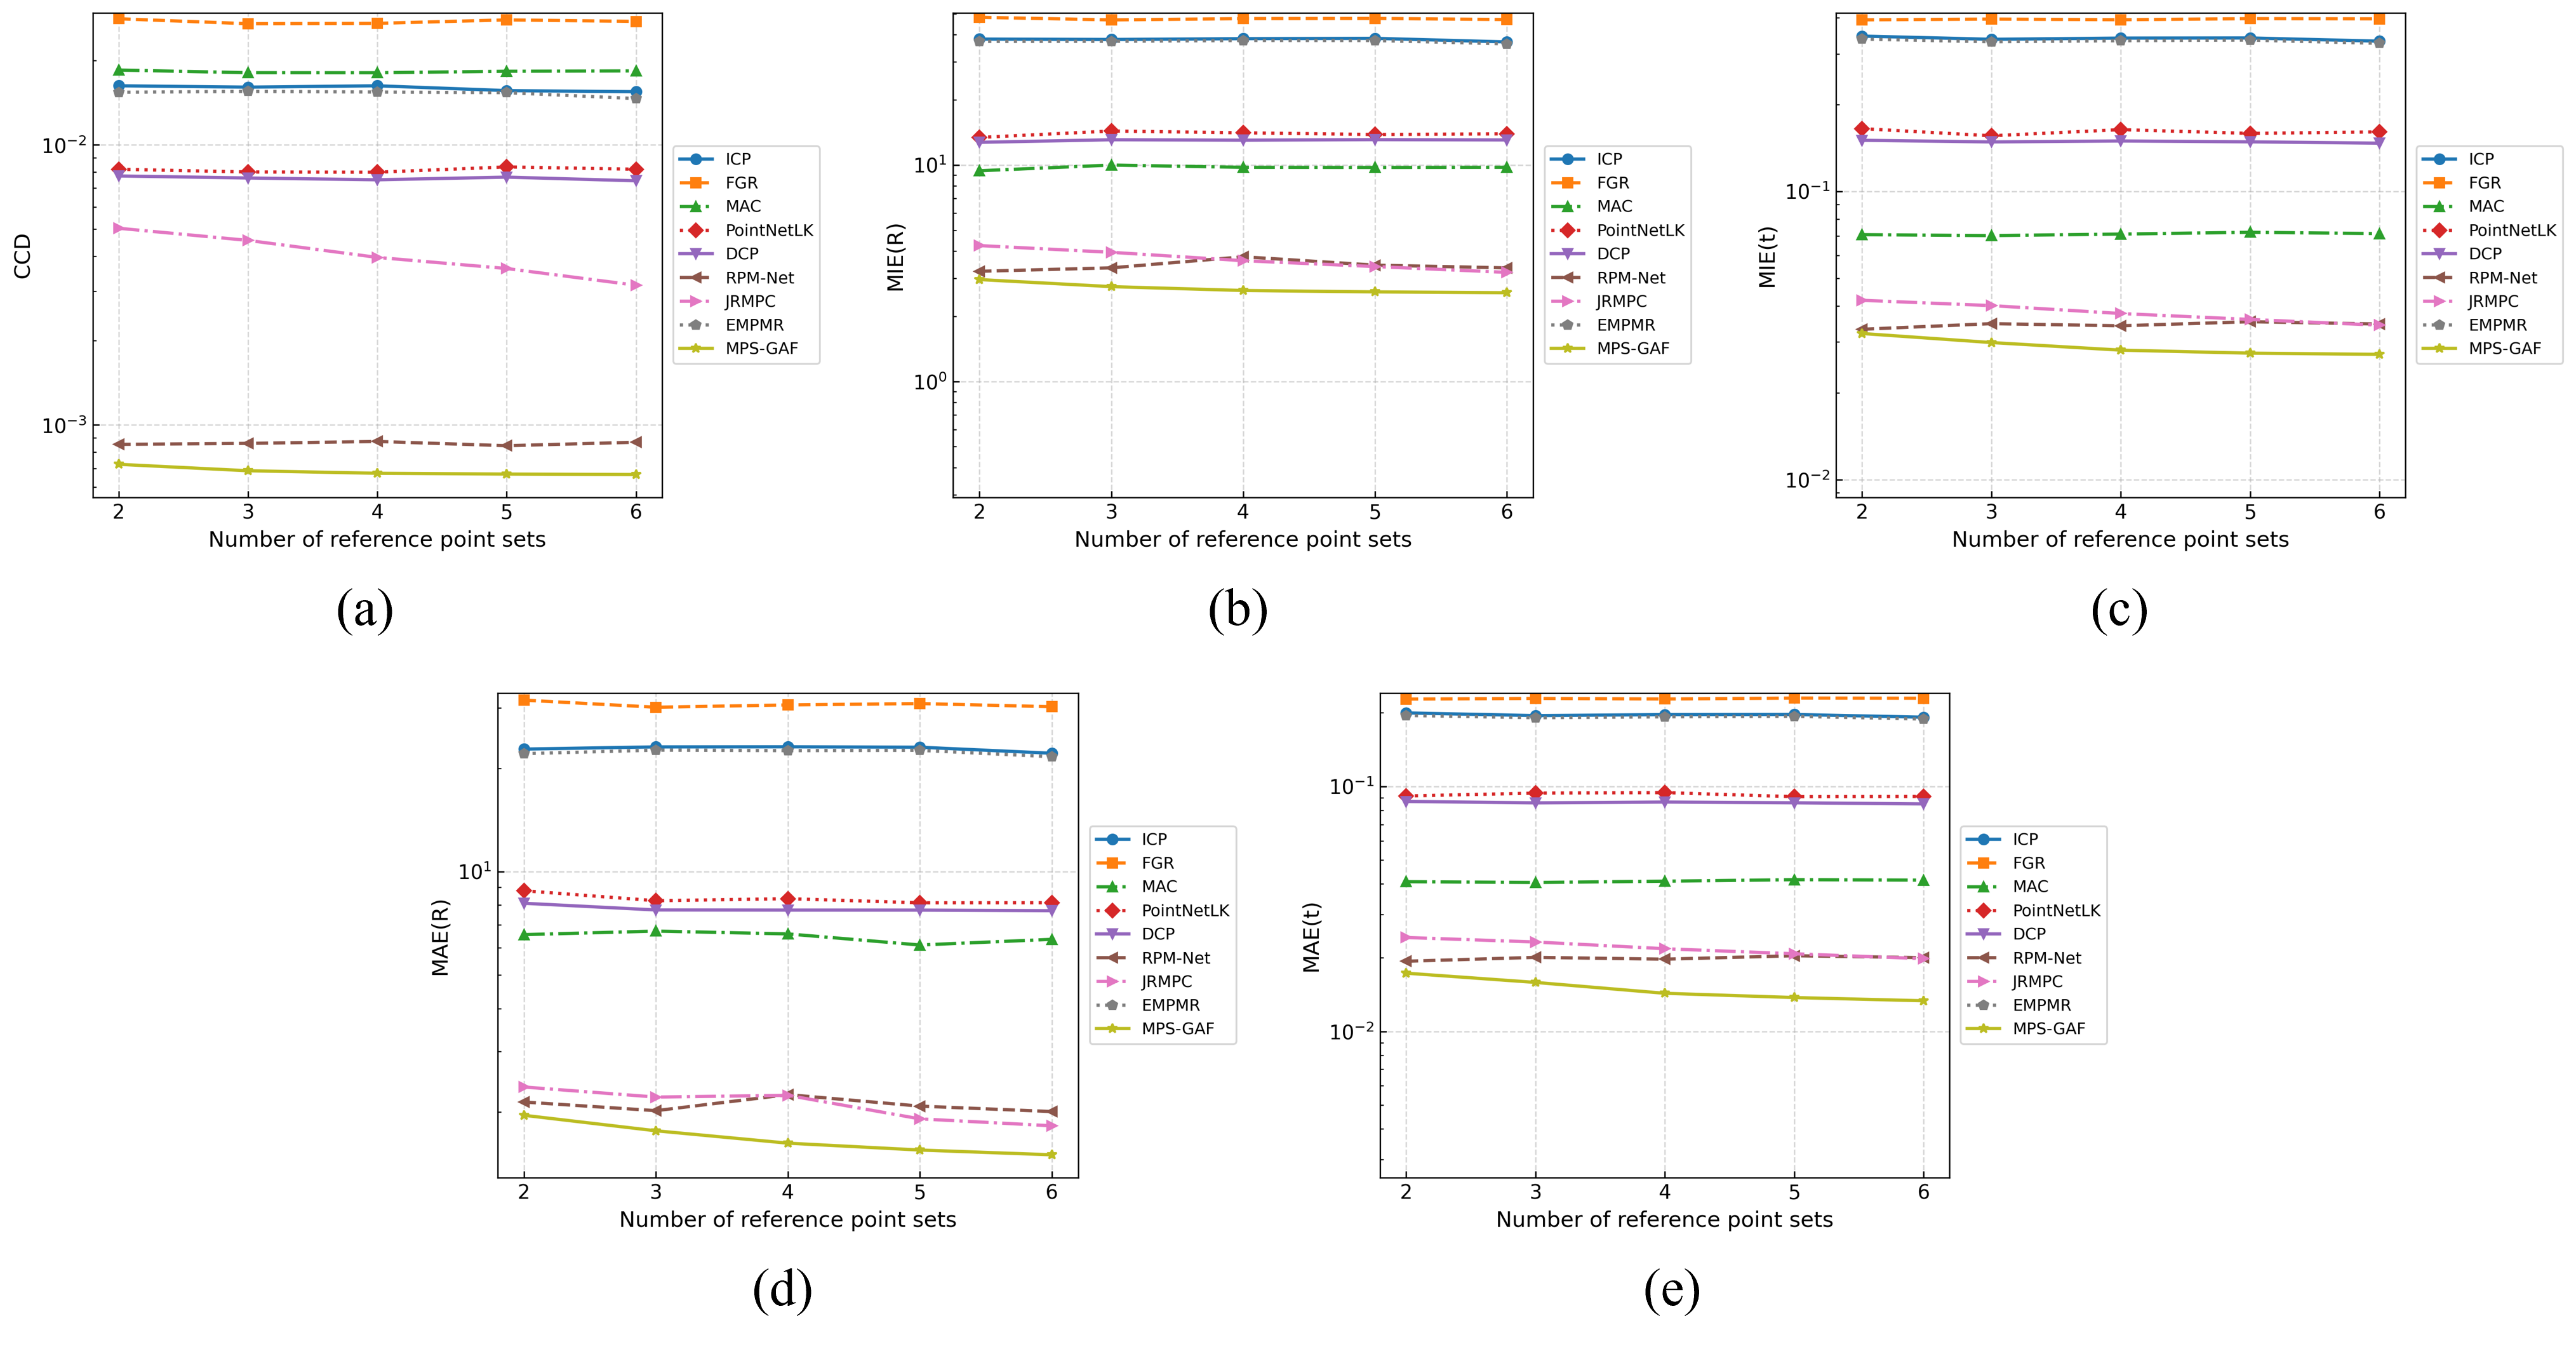
\includegraphics[width=\linewidth]{images/chapter4/registration_source_set_number.png}
  \caption{Registration performance across different numbers of source sets. The result shows that the multi-set interaction framework benefits from increasing source-set complementarity.}
  \label{fig:chapter4-numsources}
\end{figure}

The second observation concerns method generality. The results also show that the multi-set interaction module can improve several representative pairwise backbones. This is important for the present thesis because the cross-modal entity-registration stage should remain modular rather than tied to one single encoder or matcher. Table~\ref{tab:chapter4-backbone} and Fig.~\ref{fig:chapter4-backbone} summarize the evidence that the framework remains effective across multiple backbones under difficult conditions.

\begin{table}[H]
  \centering
  \caption{Performance gain across different backbone networks under difficult conditions.}
  \label{tab:chapter4-backbone}
  \begin{tabular}{lccccc}
    \toprule
    Method & MIE(R) & MIE(t) & MAE(R) & MAE(t) & CCD \\
    \midrule
    DCP & 34.431 & 0.478 & 20.450 & 0.275 & 0.0443 \\
    DCP + MPS-GAF & \textbf{29.074} & \textbf{0.397} & \textbf{16.824} & \textbf{0.229} & \textbf{0.0333} \\
    PointNetLK & 51.315 & 0.562 & 29.671 & 0.324 & 0.0681 \\
    PointNetLK + MPS-GAF & \textbf{45.828} & \textbf{0.535} & \textbf{26.493} & \textbf{0.309} & \textbf{0.0601} \\
    RPM-Net & 35.063 & 0.391 & 25.363 & 0.225 & 0.0113 \\
    RPM-Net + MPS-GAF & \textbf{30.124} & \textbf{0.343} & \textbf{22.531} & \textbf{0.202} & \textbf{0.0103} \\
    \bottomrule
  \end{tabular}
\end{table}

The table gives the quantitative evidence for the modularity of the framework. The following visual comparison complements this evidence by showing the same trend in registration quality under representative backbone choices.

\begin{figure}[htb]
  \centering
  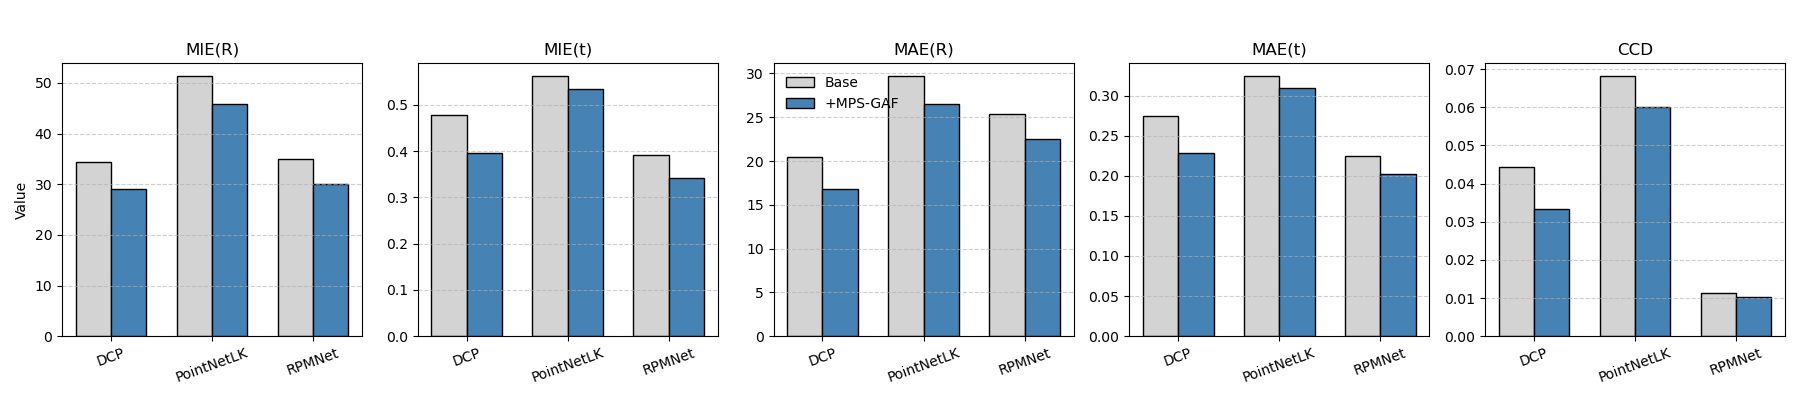
\includegraphics[width=0.9\linewidth]{images/chapter4/registration_backbone_comparison.png}
  \caption{Comparison of the multi-set graph matching framework across different backbones. The result shows that the reliability-aware multi-set interaction mechanism consistently improves several representative pairwise registration networks.}
  \label{fig:chapter4-backbone}
\end{figure}

At the same time, the experimental analysis also reveals the limitation of the present approach. If the trajectory embeddings are too weak, or if all source sets are simultaneously degraded, then even relation-aware matching may remain uncertain. In addition, the final fusion quality still depends on the quality of the completed trajectories supplied by the upstream modules. These limitations do not invalidate the present chapter, but they clarify the conditions under which multi-set registration is most effective and motivate later extensions that can further strengthen trajectory encoding and confidence modeling.

\section{Chapter Summary}
This chapter studies multimodal target fusion from the perspective of cross-modal entity registration. First, completed trajectories from different modalities are converted into a unified target-centered representation and encoded into compact trajectory embeddings. Second, a multi-set graph matching framework refines these embeddings through intra-set interaction and cross-set information exchange. Third, a reliability-aware gated fusion mechanism adaptively weights heterogeneous matching evidence and produces soft entity-level correspondences across modality-specific entity sets. Finally, the registered entities are merged into unified fused target representations, which serve as the input to the behavior analysis tasks in the next chapter.

\chapter{Behavior Analysis Based on Fused Multimodal Data}

\section{Introduction}
Chapter 4 established entity-level correspondences across heterogeneous modalities and produced a unified representation for each physical target. This representation retains trajectory information together with modality-specific attributes, making it richer than a single-source track. However, target fusion does not by itself determine whether an entity behaves normally. In monitoring scenarios, the system must also judge whether a target follows a plausible route, whether its speed and motion shape deviate from normal patterns, and whether its behavior remains coherent with nearby targets.

This chapter studies behavior anomaly detection for the fused entities generated in Chapter 4. The setting differs from conventional trajectory anomaly detection in two respects. First, the input is an object-aligned fused entity rather than a trajectory from one sensor. Its observations may come from optical, thermal, electromagnetic, SAR, or other modalities with different visibility and sampling characteristics. Second, abnormality may appear at multiple semantic levels. A target may be individually abnormal because its route, speed, or motion shape is unusual. It may also be group-wise abnormal when it departs from the local motion pattern of neighboring targets.

This chapter asks how object-aligned multimodal fusion results can be converted into reproducible anomaly evidence at the individual, group, and situation levels. To address this question, behavior analysis is organized into an individual-level detector, a group-level detector, and a score-fusion stage that projects object-level evidence into situation-level outputs. The individual-level detector follows a route-speed-shape design. Fused trajectories are converted into route, speed, and shape feature sequences, and an LSTM autoencoder learns the normal pattern of each feature type. Reconstruction errors are then adjusted by embedding-space neighborhoods, and multiple detector outputs are fused by rank-based ensemble scoring.

\section{Related Work}

\subsection{Trajectory-Based Anomaly Detection}
Trajectory-based behavior analysis studies how motion traces reflect normal movement patterns, abnormal deviations, and high-level target activities. Early trajectory mining methods relied mainly on geometric similarity, density statistics, clustering, and local trajectory segmentation. Representative work such as TRACLUS partitions trajectories into meaningful line segments and groups similar sub-trajectories to discover common movement patterns \cite{lee2007traclus}. The partition-and-detect framework further showed that abnormal behavior may appear in a local part of a trajectory rather than across the entire track \cite{lee2008traod}. Isolation-based trajectory anomaly detection demonstrated that unusual routes can be identified by measuring how easily a trajectory can be isolated from normal movement patterns \cite{zhang2011ibat}. These classical methods provide the basic intuition for this chapter: abnormal behavior should be analyzed from the full trajectory, local motion segments, speed changes, direction shifts, and route-level deviations.

With the development of deep representation learning, trajectory anomaly detection has moved from manually designed distances toward learned normal-pattern modeling. Recent studies attempt to model more complex trajectory distributions and richer abnormality types. CETrajAD explicitly decomposes trajectory anomalies into route, speed, and shape aspects and combines complementary detectors for different anomaly types \cite{cao2025cetrajectory}. DiffTAD introduces diffusion-based denoising for vehicle trajectory anomaly detection, treating anomaly detection as the reconstruction of a normal trajectory distribution from corrupted observations \cite{li2024difftad}. Context-aware trajectory anomaly detection further argues that coordinates alone are insufficient, and incorporates agent identity and geographic context into the reconstruction process \cite{hu2024contexttrajad}. More recently, graph-enhanced trajectory anomaly detection integrates movement-network topology, segment semantics, historical transition patterns, and confidence-weighted anomaly scoring \cite{mbuya2025getad}. These studies indicate that modern trajectory behavior analysis increasingly combines motion features, contextual semantics, and structural constraints.

The above work is highly relevant to the present thesis, but most existing methods still assume that the input trajectory is produced by a single observation source or by a relatively fixed movement network. In contrast, the behavior analysis problem considered here uses the fused entity representation generated in Chapter 4. Each entity contains both a trajectory component and modality-specific attributes. The behavior representation in this chapter therefore preserves useful motion descriptors from classical trajectory analysis while carrying forward multimodal information from the upstream fusion stage.

\subsection{Graph-Based Group Anomaly Detection}
Individual trajectory features are insufficient when the behavior of a target is constrained by surrounding targets. Early multi-agent trajectory models already recognized this issue. Social LSTM introduced social pooling to aggregate neighboring pedestrian information for trajectory prediction \cite{alahi2016sociallstm}, while Social GAN modeled socially plausible multimodal future trajectories \cite{gupta2018socialgan}. Graph-based methods then provided a more explicit way to describe target relations. Social-STGCNN represents pedestrians as graph nodes and models their interactions through spatio-temporal graph convolution \cite{mohamed2020socialstgcnn}. Trajectron++ extends this idea to heterogeneous agents and dynamically feasible prediction \cite{salzmann2020trajectronpp}, and AgentFormer uses agent-aware Transformer attention to jointly model social and temporal dependencies \cite{yuan2021agentformer}. These methods show that group behavior is better represented as a structured interaction process rather than as a set of independent trajectories.

Recent work further extends graph-based behavior modeling toward scene-aware, dynamic, and cooperative settings. SIF-TF combines past trajectories, social interaction, and semantic scene information through a scene-interaction fusion Transformer \cite{gao2024siftf}. Difficulty-guided feature enhancement emphasizes that different agents have different prediction difficulty and strengthens the representation of difficult agents \cite{xin2024dgfnet}. For cooperative driving, Co-MTP uses cooperative perception and multi-temporal fusion to model trajectory evolution in autonomous-driving scenes \cite{zhang2025comtp}. For aircraft trajectories, DA-STGCN models four-dimensional trajectory prediction through spatiotemporal feature extraction \cite{kuang2025dastgcn}. These recent studies are especially useful for this chapter because they treat interaction relations as dynamic and scene-dependent, which is consistent with the target groups considered in multimodal behavior analysis.

However, most of these graph-based studies focus on trajectory forecasting. Their objective is usually to predict future positions, whereas this chapter aims to describe behavior consistency, detect abnormal changes, and support situation interpretation. This chapter therefore adopts the graph representation idea for behavior analysis. Fused entities are treated as graph nodes, spatial proximity and motion correlation are encoded as edges, and graph evolution is used to measure whether a target remains consistent with its surrounding group.

\subsection{Anomaly Score Fusion and Situation Visualization}
Object-level anomaly detection is useful for monitoring only when its evidence can be fused, interpreted, and returned to the scene. Classical situation-awareness theory distinguishes object perception from situation comprehension and projection \cite{endsley1995situation}. Multisensor data fusion research makes a similar distinction between target-level estimation and higher-level situation assessment \cite{hall1997multisensor,blasch2009blueprint}. This distinction is consistent with the architecture of this thesis. Chapter 4 produces fused entities, whereas this chapter converts their behavior evidence into anomaly decisions and spatial situation indicators.

Recent graph-based anomaly detection offers practical mechanisms for this conversion. MTAD-GAT combines feature-oriented and temporal graph attention for multivariate time-series anomaly detection \cite{zhao2020mtadgat}. GDN learns a graph of variable dependencies and detects deviations through prediction errors \cite{deng2021gdn}. For multimodal time series, MST-GAT uses spatial-temporal graph attention to model dependencies within and across modalities \cite{ding2023mstgat}. GST-Pro further considers missing values and irregular observations through a graph spatio-temporal process and distribution-based scoring \cite{zheng2024gstpro}. These studies show that anomaly scores can be obtained from abnormal dependencies, not only from isolated reconstruction errors.

The final step is to make these scores interpretable at the situation level. Traditional hotspot analysis uses kernel density estimation or spatio-temporal kernel density estimation to map discrete events into continuous regional intensity fields. Spatio-temporal KDE has been used for predictive hotspot mapping and evaluation \cite{hu2018stkde}. Cyclically adjusted STKDE further incorporates temporal periodicity into hotspot prediction \cite{han2023cstkde}. Recent deep models learn multi-scale spatio-temporal dependencies for hotspot map prediction \cite{jing2024sthgnet}. Temporal network KDE improves KDE computation on road networks with multiple time periods \cite{shao2025tnkde}. These studies indicate that a situation heatmap should represent score-weighted risk rather than target density alone.

Taken together, prior studies provide useful tools for anomaly modeling, graph dependency analysis, and hotspot visualization. Less attention has been paid to how these components can be connected when the basic analysis unit is not a single-source trajectory but a fused entity produced by upstream multimodal registration. This chapter addresses this operational gap by estimating individual and group anomaly evidence from fused trajectories and projecting the resulting scores into quantitative situation indicators.

\section{Problem Definition}
Let \(\mathcal{O}=\{e_1,e_2,\ldots,e_N\}\) denote the fused object set generated by the multimodal target fusion module in Chapter 4. Following the notation of Chapter 4, each fused entity \(e_i\) corresponds to one physical target after cross-modal registration and can be written as
\begin{equation}
  e_i=\{T_i,F_i,C_i\},
\end{equation}
where \(T_i\) denotes the fused trajectory component, \(F_i\) denotes fused modality-specific attributes, and \(C_i\) denotes the confidence information inherited from the registration stage. For behavior analysis, the trajectory component is further written as a time-ordered behavior-state sequence
\begin{equation}
  T_i=\{\chi_{i,1},\chi_{i,2},\ldots,\chi_{i,L_i}\},
\end{equation}
where \(L_i\) is the trajectory length. At time \(t\), the behavior state \(\chi_{i,t}\) contains the fused position, motion-related information, and fused attributes:
\begin{equation}
  \chi_{i,t}=\big[p_{i,t},\,v_{i,t},\,f_{i,t}^{\mathrm{fuse}}\big],
\end{equation}
where \(p_{i,t}\) denotes the fused spatial position, \(v_{i,t}\) denotes fused motion information, and \(f_{i,t}^{\mathrm{fuse}}\) denotes the fused attribute representation. The source fragments that support this fused entity are retained for traceability:
\begin{equation}
  \mathcal{T}_i^{\mathrm{src}}=\{\tau_i^{(m)} \mid m\in\mathcal{M}_i\},
\end{equation}
where \(\mathcal{M}_i\) is the set of available modalities for entity \(i\), and \(\tau_i^{(m)}\) denotes the trajectory fragment observed by modality \(m\). In this chapter, however, individual anomaly detection is performed on the fused trajectory \(T_i\), rather than on separate modality-specific fragments. In the individual-level detector, only the trajectory-derived part of \(T_i\) is used to construct route, speed, and shape features. The fused attributes \(F_i\) and confidence information \(C_i\) are retained for traceability and later score interpretation, but they are not treated as independent detector branches in this section.

The objective of this chapter is to estimate anomaly evidence from these fused entities. For each target \(e_i\), the individual-level detector estimates a score \(S_i^{\mathrm{ind}}\), which measures whether the target's own motion pattern is abnormal relative to normal route, speed, and shape distributions. The group-level detector estimates a score \(S_i^{\mathrm{grp}}\), which measures whether the target is inconsistent with the spatio-temporal behavior of its local neighbors. The final behavior analysis stage combines these scores into an object-aligned anomaly score \(S_i\) and an event decision \(y_i\):
\begin{equation}
  S_i = \Psi\big(S_i^{\mathrm{ind}},S_i^{\mathrm{grp}}\big), \qquad
  y_i = \mathbb{I}(S_i>\theta),
\end{equation}
where \(\Psi(\cdot)\) is the score-fusion function, \(\theta\) is the anomaly decision threshold, and \(\mathbb{I}(\cdot)\) is the indicator function. In addition to object-level scores, anomaly evidence can be accumulated over space and time to produce a regional situation field \(\Xi(x,y,t)\). The output of this chapter therefore includes individual anomaly scores, group anomaly scores, fused anomaly decisions, and spatial situation indicators.

\section{Individual-Level Anomaly Detection}

Individual-level anomaly detection evaluates whether the motion pattern of a single fused entity is unusual without using group context. This design is useful because many abnormal behaviors are visible in the target trajectory itself, such as taking an uncommon route, moving with an unusual speed profile, or exhibiting an irregular motion shape. Because the multimodal fusion module has already produced object-aligned trajectories, this section applies the route-speed-shape detection design to the fused trajectory \(T_i\). As shown in Figure~\ref{fig:chapter5-route-speed-shape-feature}, the fused trajectory is decomposed into route, speed, and shape representations. One LSTM autoencoder detector is trained for each representation, and the detector outputs are fused into an individual anomaly score.

\begin{figure}[htbp]
  \centering
  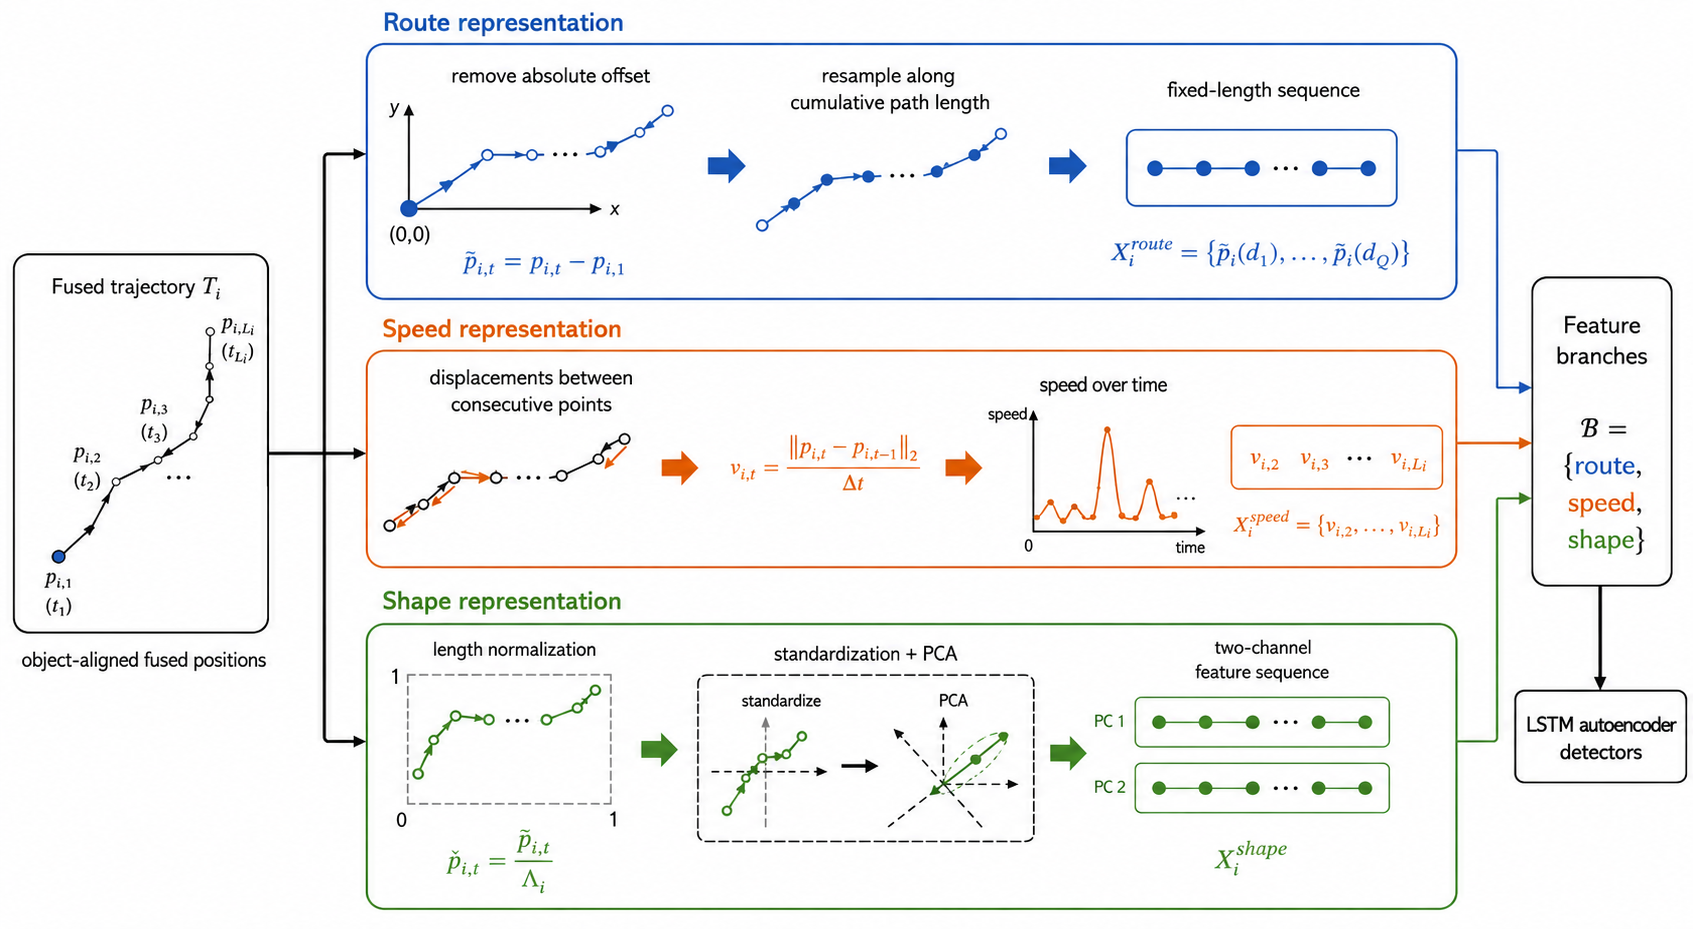
\includegraphics[width=\linewidth]{images/chapter5/route_speed_shape_feature_construction.png}
  \caption{Route, speed, and shape feature construction from a fused target trajectory. The fused trajectory is converted into a route sequence by removing the initial offset and resampling along cumulative distance, a speed sequence by frame-wise displacement over elapsed time, and a shape sequence by length normalization, standardization, and principal component projection.}
  \label{fig:chapter5-route-speed-shape-feature}
\end{figure}

\subsection{Route-Speed-Shape Feature Construction}
For a fused entity \(e_i\), let \((p_{i,t},\gamma_{i,t})\) denote the \(t\)-th observation extracted from the fused trajectory \(T_i\), where \(p_{i,t}=[x_{i,t},y_{i,t}]\), \(\gamma_{i,t}\) is the observation timestamp, and \(t=1,\ldots,L_i\). Feature construction is applied only when the number of valid observations and the path length exceed predefined thresholds used throughout the experiment. The numerical constant \(\epsilon\) is also fixed before testing. The first representation is the route feature, which describes the target's spatial path after removing the absolute starting position. Each point is converted into a relative coordinate
\begin{equation}
  \tilde{p}_{i,t} = p_{i,t} - p_{i,1}.
\end{equation}
The cumulative path length is then computed as
\begin{equation}
  d_{i,t}=\sum_{r=2}^{t}\left\|\tilde{p}_{i,r}-\tilde{p}_{i,r-1}\right\|_2,
\end{equation}
which gives the traveled distance from the starting point to the \(t\)-th observation. The relative trajectory is then resampled on this cumulative-distance axis to a fixed number of positions. Let \(d_q\), \(q=1,\ldots,Q\), denote uniformly selected distance values between the start and the end of the trajectory. The notation \(\tilde{p}_{i}(d_q)\) denotes the relative position obtained by linear interpolation at distance \(d_q\), rather than the position at a particular frame index. This produces a fixed-length route sequence
\begin{equation}
  X_{i}^{\mathrm{route}}=\{\tilde{p}_{i}(d_1),\tilde{p}_{i}(d_2),\ldots,\tilde{p}_{i}(d_Q)\}.
\end{equation}
Thus, fused trajectories with different frame numbers or sampling rates are converted into comparable route features. This representation emphasizes the path followed by the target and reduces sensitivity to the absolute coordinate offset between scenes.

The second representation is the speed feature. For consecutive observations in the fused trajectory, the scalar speed is estimated by
\begin{equation}
  u_{i,t}=
  \frac{\left\|p_{i,t}-p_{i,t-1}\right\|_2}
  {\max(\gamma_{i,t}-\gamma_{i,t-1},\epsilon)},
\end{equation}
where \(\epsilon\) is a small constant used to avoid numerical instability. The speed sequence is written as
\begin{equation}
  X_{i}^{\mathrm{speed}}=\{u_{i,2},u_{i,3},\ldots,u_{i,L_i}\}.
\end{equation}
Compared with the route representation, the speed representation is more sensitive to abrupt acceleration, abnormal stopping, and unusually fast movement.

The third representation is the shape feature. Shape is intended to describe the geometry of the motion rather than the absolute position or the total path length. Consecutive duplicate positions are removed first. If the remaining trajectory has a path length below the predefined threshold or is shorter than the minimum sequence length, the shape feature is treated as unavailable. Otherwise, the relative coordinates are normalized by the total path length
\begin{equation}
  \Lambda_i=\sum_{t=2}^{L_i}\left\|\tilde{p}_{i,t}-\tilde{p}_{i,t-1}\right\|_2,\qquad
  \breve{p}_{i,t}=\frac{\tilde{p}_{i,t}}{\Lambda_i}.
\end{equation}
The normalized curve is resampled along a normalized temporal axis and standardized using training-set statistics. The principal component projection is fitted on the training shape sequences only and then applied unchanged to validation and test trajectories. The resulting two-channel sequence is denoted as \(X_{i}^{\mathrm{shape}}\). The detector set therefore contains three fused-trajectory feature branches:
\begin{equation}
  \mathcal{B}=\{\mathrm{route},\mathrm{speed},\mathrm{shape}\}.
\end{equation}
The multimodal information enters this stage through the fused trajectory itself, so no separate RGB or thermal detector branch is introduced here.

\subsection{LSTM Autoencoder-Based Detector}
For each feature branch \(a\in\mathcal{B}\), all valid sequences are collected as \(\{X_i^{(a)}\}\), where \(X_i^{(a)}\in\mathbb{R}^{L_i^{(a)}\times d_a}\), \(L_i^{(a)}\) is the branch-specific sequence length, and \(d_a\) is the feature dimension. Before training, the sequence values are normalized using statistics estimated from the training split. Because different targets have different valid lengths, sequences are padded within each mini-batch and a binary mask \(M_i^{(a)}\) identifies valid time steps. The complete individual-level detection workflow is summarized in Figure~\ref{fig:chapter5-individual-anomaly-workflow}: branch-specific LSTM autoencoders provide reconstruction evidence, embedding-space neighborhoods adjust branch scores, and rank-based ensemble scoring produces the final individual anomaly score.

\begin{figure}[htbp]
  \centering
  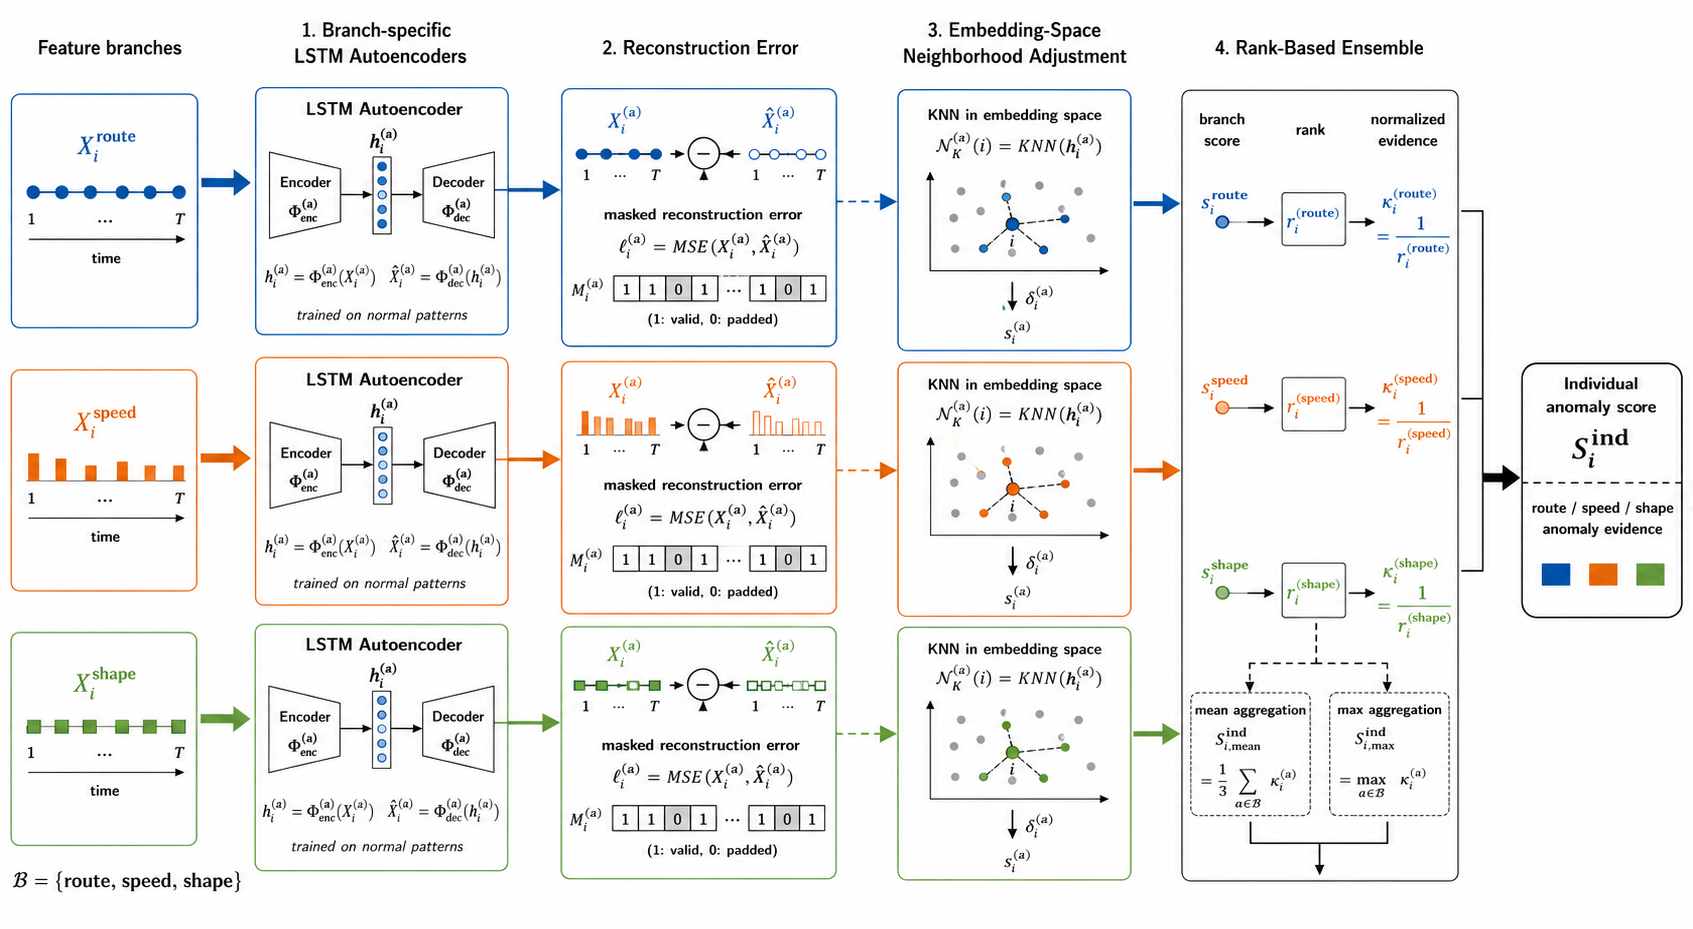
\includegraphics[width=\linewidth]{images/chapter5/individual_anomaly_detection_workflow.png}
  \caption{Individual-level anomaly detection workflow. Route, speed, and shape feature sequences are processed by branch-specific LSTM autoencoders. Masked reconstruction errors are adjusted by embedding-space neighborhoods, and branch-level scores are fused through rank-based ensemble scoring to obtain the individual anomaly score.}
  \label{fig:chapter5-individual-anomaly-workflow}
\end{figure}

Each branch is modeled by an LSTM autoencoder. The encoder maps a normalized feature sequence to a compact embedding:
\begin{equation}
  h_i^{(a)}=\Phi_{\mathrm{enc}}^{(a)}\big(X_i^{(a)}\big),
\end{equation}
where \(h_i^{(a)}\) is the latent representation of entity \(i\) under branch \(a\). The decoder repeats this latent vector along the temporal dimension and reconstructs the original sequence:
\begin{equation}
  \hat{X}_i^{(a)}=\Phi_{\mathrm{dec}}^{(a)}\big(h_i^{(a)},L_i^{(a)}\big).
\end{equation}
The model is trained to minimize the reconstruction error on valid, non-padded positions:
\begin{equation}
  \mathcal{L}^{(a)} =
  \frac{1}{|\mathcal{D}_{\mathrm{tr}}|}
  \sum_{i\in\mathcal{D}_{\mathrm{tr}}}
  \frac{
  \sum_{t=1}^{L_i^{(a)}} M_{i,t}^{(a)}
  \left\|X_{i,t}^{(a)}-\hat{X}_{i,t}^{(a)}\right\|_2^2
  }
  {
  d_a\sum_{t=1}^{L_i^{(a)}}M_{i,t}^{(a)}+\epsilon
  }.
\end{equation}
After training, the per-sample reconstruction error is used as the initial anomaly evidence:
\begin{equation}
  \ell_i^{(a)} =
  \frac{
  \sum_{t=1}^{L_i^{(a)}} M_{i,t}^{(a)}
  \left\|X_{i,t}^{(a)}-\hat{X}_{i,t}^{(a)}\right\|_2^2
  }
  {
  d_a\sum_{t=1}^{L_i^{(a)}}M_{i,t}^{(a)}+\epsilon
  }.
\end{equation}
A high value of \(\ell_i^{(a)}\) indicates that the corresponding route, speed, or shape sequence is difficult to reconstruct using the normal-pattern model.

\subsection{Neighborhood-Adjusted Anomaly Score}
Directly using reconstruction error may be unstable when some normal trajectory groups are intrinsically difficult to reconstruct. To reduce this effect, the detector adjusts the reconstruction error by comparing each trajectory with its nearest neighbors in the learned embedding space. For branch \(a\), the neighborhood of entity \(i\) is defined as
\begin{equation}
  \mathcal{N}_K^{(a)}(i)=
  \operatorname{KNN}
  \big(h_i^{(a)},
  \{h_j^{(a)}\mid j\in\mathcal{D}_{\mathrm{ref}}^{(a)}, j\neq i\},K\big),
\end{equation}
where \(K\) is the number of neighbors and \(\mathcal{D}_{\mathrm{ref}}^{(a)}\) denotes a fixed reference embedding set, such as the normal training set or a historical reference set. This prevents the neighborhood adjustment from depending on the composition of a test batch. The local loss deviation of entity \(i\) is then computed as
\begin{equation}
  \delta_i^{(a)}=
  \frac{1}{|\mathcal{N}_K^{(a)}(i)|}
  \sum_{j\in\mathcal{N}_K^{(a)}(i)}
  \left|\ell_i^{(a)}-\ell_j^{(a)}\right|.
\end{equation}
This term measures whether the reconstruction error of the target is unusual compared with trajectories that have similar latent motion patterns. The final branch-level anomaly score is normalized by the average local deviation of its neighbors:
\begin{equation}
  s_i^{(a)}=
  \frac{\delta_i^{(a)}}
  {
  \frac{1}{|\mathcal{N}_K^{(a)}(i)|}
  \sum_{j\in\mathcal{N}_K^{(a)}(i)}\delta_j^{(a)}+\epsilon
  }.
\end{equation}
If the neighborhood is too small or the denominator is numerically close to zero, the unnormalized local deviation is used as a fallback. In this way, a trajectory receives a high branch-level score only when its reconstruction behavior is locally inconsistent with similar trajectories, not merely when its raw reconstruction loss is large.

\subsection{Multi-Representation Detector Ensemble}
The above process produces one score vector for each valid branch \(a\in\mathcal{B}\). Because route, speed, and shape features have different validity requirements, the detector outputs are first aligned by fused entity identifier. If a branch does not produce a score for a target, for example because the fused trajectory is too short or its path length is below the predefined threshold, the missing value is filled with the median score of that branch. This keeps all valid fused entities in the ensemble while avoiding an overly strong missing-value penalty.

The scores from different branches are not directly comparable in scale, so the ensemble uses rank-based normalization. Let \(r_i^{(a)}\) denote the descending rank of \(s_i^{(a)}\) among all targets in branch \(a\), where a smaller rank means a more suspicious target. The normalized branch evidence is defined as
\begin{equation}
  \kappa_i^{(a)}=\frac{1}{r_i^{(a)}}.
\end{equation}
Two aggregate scores are then computed:
\begin{equation}
  S_{i,\mathrm{mean}}^{\mathrm{ind}}=
  \frac{1}{|\mathcal{B}|}\sum_{a\in\mathcal{B}}\kappa_i^{(a)},\qquad
  S_{i,\mathrm{max}}^{\mathrm{ind}}=
  \max_{a\in\mathcal{B}}\kappa_i^{(a)}.
\end{equation}
The mean score reflects consistent evidence across multiple representations, while the max score preserves strong complementary evidence from any single route, speed, or shape branch. The final individual-level anomaly score used in the fusion stage is defined as
\begin{equation}
  S_i^{\mathrm{ind}}=S_{i,\mathrm{mean}}^{\mathrm{ind}}.
\end{equation}
The max score \(S_{i,\mathrm{max}}^{\mathrm{ind}}\) is retained as a complementary diagnostic score for branch-specific anomalies. The implementation also records a complementary elimination process. At each iteration, one detector is removed and the change in the Top-\(K\) anomaly set is measured by Jaccard similarity. Detectors whose removal causes little change are considered redundant, and the resulting curve helps analyze the contribution of each feature branch.

\section{Group-Level Spatio-Temporal Graph Anomaly Detection}

The individual-level detector evaluates whether a fused trajectory is unusual by itself. Some abnormal behaviors, however, are relational. A target may leave a stable group, move against nearby targets, or appear in a group whose population changes suddenly. To keep this part simple and interpretable, this section uses a lightweight spatio-temporal graph to describe local group relations and computes group anomaly scores from graph-structure changes and group statistics. As summarized in Figure~\ref{fig:chapter5-lightweight-st-graph-events}, fused target states are first organized as target-frame nodes with spatial and temporal edges. Connected components are then tracked as groups, and interpretable object-to-group and group-level event indicators are fused into group anomaly scores. No manually labeled group anomaly categories are required.

\begin{figure}[htbp]
  \centering
  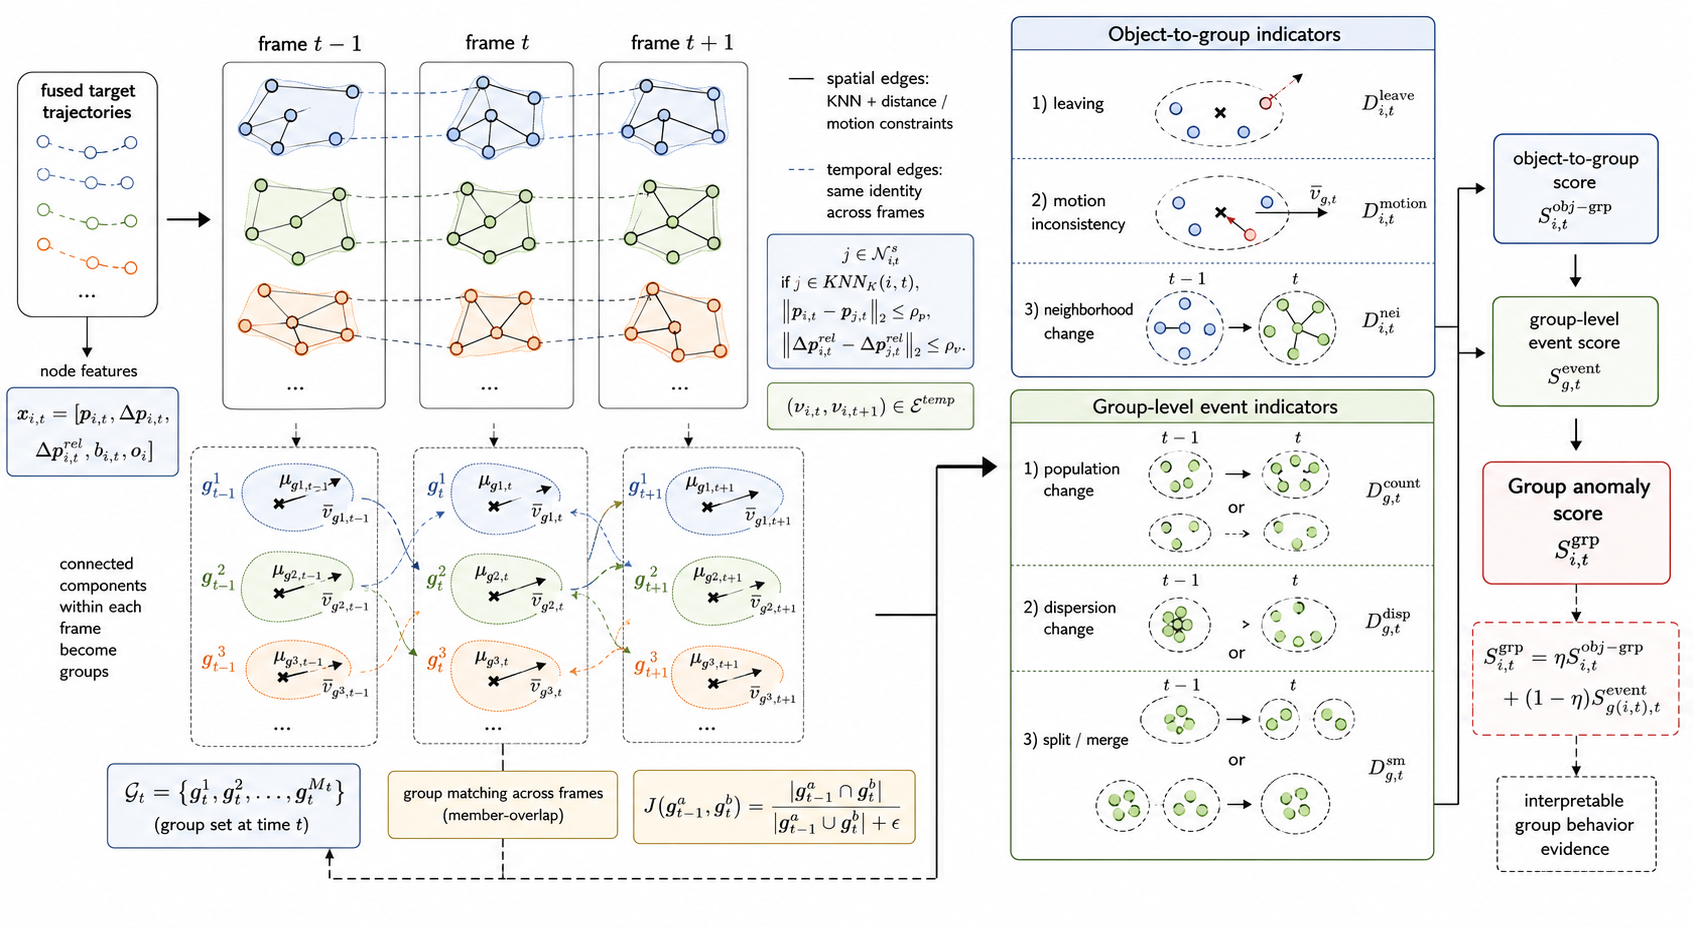
\includegraphics[width=\linewidth]{images/chapter5/lightweight_spatiotemporal_graph_group_events.png}
  \caption{Lightweight spatio-temporal graph and group event indicators. Fused target states are represented as target-frame nodes. Spatial edges describe local motion-consistent neighborhoods, and temporal edges preserve identity continuity. Connected components define candidate groups, while interpretable indicators describe object-to-group deviations and group-level events such as leaving, motion inconsistency, population change, dispersion change, split, and merge.}
  \label{fig:chapter5-lightweight-st-graph-events}
\end{figure}

\subsection{Spatio-Temporal Graph Construction}
For a sequence of frames, a sliding temporal window is defined as
\begin{equation}
  \mathcal{W}_t = \{t-L_{\mathrm{in}}+1,\ldots,t\},
\end{equation}
where \(L_{\mathrm{in}}\) is the input window length. Each visible fused target at each frame is represented as a target-frame node \(\nu_{i,\tau}\), where \(i\) denotes the target identity and \(\tau\in\mathcal{W}_t\). The node feature is constructed from the fused trajectory and basic target attributes:
\begin{equation}
  x_{i,\tau}=
  \big[p_{i,\tau},\,\Delta p_{i,\tau},\,\Delta p^{\mathrm{rel}}_{i,\tau},\,b_{i,\tau},\,o_i\big],
\end{equation}
where \(p_{i,\tau}\) is the fused target center, \(\Delta p_{i,\tau}=p_{i,\tau}-p_{i,\tau-1}\) is the target displacement, \(b_{i,\tau}\) denotes the bounding-box size, and \(o_i\) is the one-hot category vector. Because VT-Tiny-MOT is captured from aerial platforms, frame-level camera motion may cause many targets to move coherently in image coordinates. To reduce this effect, the relative displacement is defined as
\begin{equation}
  \Delta p^{\mathrm{rel}}_{i,\tau}
  =
  \Delta p_{i,\tau}
  -
  \mathrm{median}_{j\in\mathcal{V}_{\tau}}\big(\Delta p_{j,\tau}\big),
\end{equation}
where \(\mathcal{V}_{\tau}\) is the set of visible targets at frame \(\tau\). This term makes the graph focus on target motion relative to the local scene rather than on global image displacement.

The graph contains spatial edges and temporal edges. Spatial edges are constructed within each frame by a simple \(K\)-nearest-neighbor rule with distance and motion constraints:
\begin{equation}
  j\in\mathcal{N}_{i,\tau}^{s}
  \Longleftrightarrow
  j\in\operatorname{KNN}_{K}(i,\tau),\quad
  \|p_{i,\tau}-p_{j,\tau}\|_2\leq\rho_p,\quad
  \|\Delta p^{\mathrm{rel}}_{i,\tau}-\Delta p^{\mathrm{rel}}_{j,\tau}\|_2\leq\rho_v.
\end{equation}
Here \(\rho_p\) and \(\rho_v\) control the maximum spatial distance and relative-motion difference allowed for a local group relation. In implementation, \(p_{i,\tau}\) and \(\Delta p^{\mathrm{rel}}_{i,\tau}\) are measured in the unified plane provided by the fusion module. The parameters \(K\), \(\rho_p\), and \(\rho_v\) are fixed on the validation split and then kept unchanged for all test sequences. Temporal edges connect the same target across adjacent frames:
\begin{equation}
  \mathcal{E}^{\mathrm{temp}}=\{(\nu_{i,\tau},\nu_{i,\tau+1})\mid i \text{ is visible at both } \tau \text{ and } \tau+1\}.
\end{equation}
This graph is intentionally simpler than the relation-aware graph in Chapter 4. Chapter 4 uses graph reasoning for cross-modal entity fusion, whereas this chapter uses the graph to describe local behavior relations after fusion has been completed.

\subsection{Group Discovery and Event Indicators}
The spatial graph at each frame provides a direct basis for discovering target groups. Connected components in the spatial graph are treated as candidate groups:
\begin{equation}
  \mathcal{G}_{\tau}=\{g_{\tau}^{1},g_{\tau}^{2},\ldots,g_{\tau}^{M_{\tau}}\},
\end{equation}
where each group \(g_{\tau}^{m}\subseteq\mathcal{V}_{\tau}\) contains targets that are spatially close and motion-consistent at frame \(\tau\). Isolated targets are kept as single-target components, because isolation itself may be useful evidence for anomaly detection.

To describe group evolution across time, groups in adjacent frames are matched by member overlap. For two candidate groups \(g_{\tau-1}^{a}\) and \(g_{\tau}^{b}\), their temporal continuity score is
\begin{equation}
  J(g_{\tau-1}^{a},g_{\tau}^{b})
  =
  \frac{|g_{\tau-1}^{a}\cap g_{\tau}^{b}|}
  {|g_{\tau-1}^{a}\cup g_{\tau}^{b}|+\epsilon}.
\end{equation}
A temporal match is accepted when \(J(\cdot)\) is greater than the overlap threshold \(\theta_J\), which is fixed before testing. If a group in frame \(\tau\) has one accepted predecessor, it is considered a continuation of the previous group and inherits its propagated group identity. If one previous group corresponds to multiple current groups, a split event is recorded. If multiple previous groups correspond to one current group, a merge event is recorded. If a group has no reliable predecessor or successor, it is interpreted as group appearance or disappearance.

For each group \(g_{\tau}\), several interpretable group statistics are computed:
\begin{equation}
  n_{g,\tau}=|g_{\tau}|,\qquad
  \mu_{g,\tau}=\frac{1}{n_{g,\tau}}\sum_{i\in g_{\tau}}p_{i,\tau},
\end{equation}
\begin{equation}
  \delta_{g,\tau}=
  \frac{1}{n_{g,\tau}}\sum_{i\in g_{\tau}}\|p_{i,\tau}-\mu_{g,\tau}\|_2,
  \qquad
  \bar{v}_{g,\tau}=
  \frac{1}{n_{g,\tau}}\sum_{i\in g_{\tau}}\Delta p^{\mathrm{rel}}_{i,\tau}.
\end{equation}
Here \(n_{g,\tau}\) measures group size, \(\mu_{g,\tau}\) is the group center, \(\delta_{g,\tau}\) describes group dispersion, and \(\bar{v}_{g,\tau}\) describes group-level motion. These statistics provide interpretable evidence for distinguishing whether an anomaly is caused by an individual leaving the group, a group changing its population, or a structural event such as splitting or merging.

\subsection{Interpretable Group Anomaly Score}
The group detector converts the above graph statistics into a small set of interpretable anomaly scores. Let \(g(i,t)\) be the group containing target \(i\) at frame \(t\). The group-leaving score is defined as
\begin{equation}
  D_{i,t}^{\mathrm{leave}}
  =
  \left[
  \frac{
  \|p_{i,t}-\mu_{g(i,t),t}\|_2
  -
  \mathrm{median}_{\tau\in[t-W,t-1]}
  \|p_{i,\tau}-\mu_{g(i,\tau),\tau}\|_2
  }
  {
  \mathrm{MAD}_{\tau\in[t-W,t-1]}
  \|p_{i,\tau}-\mu_{g(i,\tau),\tau}\|_2+\epsilon
  }
  \right]_{+},
\end{equation}
where \([\cdot]_+=\max(\cdot,0)\). This score becomes high when a target moves farther away from its historical group center. The motion-inconsistency score is
\begin{equation}
  D_{i,t}^{\mathrm{motion}}
  =
  1-
  \frac{
  \langle \Delta p^{\mathrm{rel}}_{i,t},\bar{v}_{g(i,t),t}\rangle
  }
  {
  \|\Delta p^{\mathrm{rel}}_{i,t}\|_2\|\bar{v}_{g(i,t),t}\|_2+\epsilon
  },
\end{equation}
which detects targets moving against or away from the group direction. The neighborhood-change score is
\begin{equation}
  D_{i,t}^{\mathrm{nei}}
  =
  1-
  \frac{
  |\mathcal{N}_{i,t}^{s}\cap\mathcal{N}_{i,t-1}^{s}|
  }
  {
  |\mathcal{N}_{i,t}^{s}\cup\mathcal{N}_{i,t-1}^{s}|+\epsilon
  }.
\end{equation}
This term captures sudden neighbor replacement, which may correspond to leaving, entering, crossing, or merging with a group.

Group-level event deviation is measured for tracked groups whose identities are propagated through the overlap-based matching rule. For a tracked group \(g\), the population-change score is
\begin{equation}
  D_{g,t}^{\mathrm{count}}
  =
  \frac{
  |n_{g,t}-\mathrm{median}_{\tau\in[t-W,t-1]}n_{g,\tau}|
  }
  {
  \mathrm{MAD}_{\tau\in[t-W,t-1]}n_{g,\tau}+\epsilon
  },
\end{equation}
where the historical terms are computed only over frames in which the same propagated group identity is available. The dispersion-change score is
\begin{equation}
  D_{g,t}^{\mathrm{disp}}
  =
  \frac{
  |\delta_{g,t}-\mathrm{median}_{\tau\in[t-W,t-1]}\delta_{g,\tau}|
  }
  {
  \mathrm{MAD}_{\tau\in[t-W,t-1]}\delta_{g,\tau}+\epsilon
  }.
\end{equation}
The split-or-merge indicator is defined according to the same group matching results:
\begin{equation}
  D_{g,t}^{\mathrm{sm}}=
  \mathbb{I}(g \text{ is involved in a split or merge event}).
\end{equation}
These terms describe whether a group suddenly gains or loses members, becomes unusually compact or dispersed, or undergoes structural reorganization.

All component scores are robustly normalized by the median and median absolute deviation computed on the training set. Let \(\mathcal{R}(\cdot)\) denote this normalization. The weights \(\alpha_1,\alpha_2,\alpha_3,\beta_1,\beta_2,\beta_3\) are non-negative, and \(\eta\in[0,1]\). These parameters are fixed on the validation split and are not adjusted for individual test sequences. The object-to-group anomaly score is
\begin{equation}
  S_{i,t}^{\mathrm{obj\mbox{-}grp}}
  =
  \alpha_1\mathcal{R}(D_{i,t}^{\mathrm{leave}})
  +
  \alpha_2\mathcal{R}(D_{i,t}^{\mathrm{motion}})
  +
  \alpha_3\mathcal{R}(D_{i,t}^{\mathrm{nei}}).
\end{equation}
The group-event anomaly score is
\begin{equation}
  S_{g,t}^{\mathrm{event}}
  =
  \beta_1\mathcal{R}(D_{g,t}^{\mathrm{count}})
  +
  \beta_2\mathcal{R}(D_{g,t}^{\mathrm{disp}})
  +
  \beta_3D_{g,t}^{\mathrm{sm}}.
\end{equation}
Finally, the frame-level group anomaly score of target \(i\) is
\begin{equation}
  S_{i,t}^{\mathrm{grp}}
  =
  \eta S_{i,t}^{\mathrm{obj\mbox{-}grp}}
  +
  (1-\eta)S_{g(i,t),t}^{\mathrm{event}},
\end{equation}
and the object-level group anomaly score is obtained by a high-percentile aggregation:
\begin{equation}
  S_{i}^{\mathrm{grp}}
  =
  \operatorname{Percentile}_{95}
  \left(\{S_{i,t}^{\mathrm{grp}}\}_{t=1}^{L_i}\right).
\end{equation}
The dominant anomaly reason is determined by the largest normalized component in the score decomposition. For instance, a high \(D^{\mathrm{leave}}\) indicates group leaving, a high \(D^{\mathrm{nei}}\) indicates neighborhood restructuring, a high \(D^{\mathrm{count}}\) indicates sudden population change, and \(D^{\mathrm{sm}}\) directly indicates a split or merge event. Therefore, the group detector does not only output a scalar anomaly score, but also provides interpretable evidence for the type of group-level abnormal behavior.

\section{Individual-Group Fusion and Situation Output}

\subsection{Individual-Group Score Fusion}
The individual-level detector and the group-level detector describe different abnormality sources. The individual score \(S_i^{\mathrm{ind}}\) focuses on the target trajectory itself, while the group score \(S_i^{\mathrm{grp}}\) focuses on whether the target is consistent with its surrounding group and whether the group undergoes abnormal structural evolution. These two scores are therefore complementary rather than mutually exclusive. Before fusion, both scores are transformed to a comparable scale by robust normalization:
\begin{equation}
  \tilde{S}_i^{\mathrm{ind}}
  =
  \mathcal{R}\big(S_i^{\mathrm{ind}}\big),\qquad
  \tilde{S}_i^{\mathrm{grp}}
  =
  \mathcal{R}\big(S_i^{\mathrm{grp}}\big),
\end{equation}
where \(\mathcal{R}(\cdot)\) denotes median-and-MAD normalization estimated from the training split. The fused object-level anomaly score is then defined as
\begin{equation}
  S_i^{\mathrm{fuse}}
  =
  \alpha \tilde{S}_i^{\mathrm{ind}}
  +
  (1-\alpha)\tilde{S}_i^{\mathrm{grp}},
\end{equation}
where \(\alpha\in[0,1]\) controls the relative contribution of individual and group evidence. The fusion weight is selected on the validation split and is not adjusted separately for individual test sequences. When only an individual score is available, the fused score falls back to \(\tilde{S}_i^{\mathrm{ind}}\); when only a group score is available, it falls back to \(\tilde{S}_i^{\mathrm{grp}}\). This fallback design is necessary because some targets may be too short for all individual feature branches, while some frames may contain too few neighboring targets for reliable group modeling.

In addition to the scalar fused score, the fusion stage preserves the component scores:
\begin{equation}
  S_i^{\mathrm{obj\mbox{-}grp}}
  =
  \operatorname{Percentile}_{95}
  \left(\{S_{i,t}^{\mathrm{obj\mbox{-}grp}}\}_{t=1}^{L_i}\right),
  \qquad
  S_i^{\mathrm{event}}
  =
  \operatorname{Percentile}_{95}
  \left(\{S_{g(i,t),t}^{\mathrm{event}}\}_{t=1}^{L_i}\right),
\end{equation}
\begin{equation}
  \Omega_i=
  \{S_i^{\mathrm{ind}},S_i^{\mathrm{grp}},
  S_i^{\mathrm{obj\mbox{-}grp}},S_i^{\mathrm{event}}\}.
\end{equation}
The component record makes the final output interpretable. If \(S_i^{\mathrm{ind}}\) dominates, the abnormality is mainly caused by the target's own route, speed, or shape. If \(S_i^{\mathrm{obj\mbox{-}grp}}\) dominates, the abnormality is mainly a target-to-group deviation such as leaving, entering, or moving against the local group. If \(S_i^{\mathrm{event}}\) dominates, the abnormality is mainly caused by a group event such as population change, split, merge, or dispersion change.

\subsection{Anomaly Event Decision}
The fused score can fluctuate at a single frame because of detection noise, temporary occlusion, or short-term tracking instability. Therefore, event decisions are made after temporal smoothing. Let \(S_{i,t}^{\mathrm{fuse}}\) denote the frame-level fused score before target-level aggregation. A smoothed score is computed by an exponential moving average:
\begin{equation}
  \bar{S}_{i,t}^{\mathrm{fuse}}
  =
  \lambda_s\bar{S}_{i,t-1}^{\mathrm{fuse}}
  +
  (1-\lambda_s)S_{i,t}^{\mathrm{fuse}},
\end{equation}
where \(\lambda_s\in[0,1]\) controls the smoothing strength. The anomaly event decision is then defined as
\begin{equation}
  y_{i,t}
  =
  \mathbb{I}\left(
  \bar{S}_{i,t}^{\mathrm{fuse}}>\theta
  \right),
\end{equation}
where \(\theta\) is selected according to the desired false alarm level or by a fixed top-percentile rule on the validation split. The smoothing factor \(\lambda_s\) and the decision threshold \(\theta\) are fixed before testing. To avoid reporting many fragmented alarms for the same target, consecutive abnormal frames are merged into one event segment:
\begin{equation}
  \mathcal{I}_i^{\mathrm{evt}} =
  \{[t_s,t_e]\mid y_{i,t}=1,\ t_s\leq t\leq t_e\}.
\end{equation}
Each event segment is assigned an event score by the maximum or high-percentile value within the segment:
\begin{equation}
  S([t_s,t_e])
  =
  \operatorname{Percentile}_{95}
  \left(
  \{\bar{S}_{i,t}^{\mathrm{fuse}}\mid t\in[t_s,t_e]\}
  \right).
\end{equation}
The event type is determined from the largest component score inside the segment. This yields interpretable labels such as route anomaly, speed anomaly, shape anomaly, group leaving, motion inconsistency, neighborhood restructuring, population change, split, and merge.

\subsection{Situation Heatmap Generation}
The final output of behavior analysis should support situation interpretation rather than only provide object-level rankings. For this purpose, object-level anomaly evidence is projected back to the image plane or the unified spatial plane and accumulated into a regional situation heatmap. For frame \(t\), the heatmap value at location \((x,y)\) is defined as
\begin{equation}
  \Xi_t(x,y)
  =
  \sum_{i\in\mathcal{V}_t}
  \bar{S}_{i,t}^{\mathrm{fuse}}
  K_{\sigma}
  \big((x,y)-p_{i,t}\big),
\end{equation}
where \(K_{\sigma}(\cdot)\) is a Gaussian kernel with bandwidth \(\sigma\). The bandwidth is fixed for all sequences. This formulation differs from a conventional target-density map because each target is weighted by its anomaly score. Regions containing many normal targets do not necessarily become high-risk regions, while a small number of highly abnormal targets can still create a visible hotspot.

For temporal situation analysis, frame-level heatmaps can be accumulated with a decay factor:
\begin{equation}
  \bar{\Xi}_t(x,y)
  =
  \lambda_h\bar{\Xi}_{t-1}(x,y)
  +
  (1-\lambda_h)\Xi_t(x,y),
\end{equation}
where \(\lambda_h\) controls how long recent anomaly evidence remains visible and is fixed before testing. The regional situation intensity of a spatial cell \(\mathcal{P}\) is then
\begin{equation}
  I_t(\mathcal{P})
  =
  \frac{1}{|\mathcal{P}|}
  \int_{(x,y)\in\mathcal{P}}
  \bar{\Xi}_t(x,y)\,dx\,dy.
\end{equation}
This output connects object-level anomaly detection with situation-level visualization. It allows the system to identify not only which target is abnormal, but also where abnormal behavior is concentrated and how the regional risk changes over time.

\section{Experiments and Result Analysis}

\subsection{Dataset and Experimental Setting}
The experiment in this chapter uses the VT-Tiny-MOT dataset. VT-Tiny-MOT is a visible-infrared multi-object tracking dataset collected from aerial scenes. Each sequence contains paired image streams and target annotations, which makes it suitable for constructing object-centered trajectories and demonstrating downstream behavior analysis from fused target representations. The image sequences also cover different scene layouts, target densities, illumination conditions, and motion patterns. They therefore provide a practical input source for examining the visualization stage of the proposed anomaly detection framework.

This dataset is used here for two reasons. First, its tracking-oriented annotations are consistent with the input form required by this chapter: the behavior detector operates on fused trajectories rather than on isolated video frames. Second, the dataset contains multiple real aerial scenes, which makes the generated heatmaps easier to interpret at the situation level. However, VT-Tiny-MOT does not provide manually annotated individual or group anomaly labels. Therefore, the experiment in this chapter is organized as a qualitative visualization study rather than a supervised detection benchmark. Precision, recall, average precision, and other label-dependent metrics are not reported. The results are used only to examine whether object-aligned anomaly scores can be projected into interpretable scene-level heatmaps.

The test output contains ten video sequences. For each sequence, the final result is presented as an anomaly heatmap overlaid on the original scene. The heatmap is not a target-density map or a manual abnormal-region annotation. Each target point contributes to nearby spatial regions according to its anomaly score, so a high-value region means that model-derived anomaly evidence is spatially concentrated there.

\subsection{Qualitative Heatmap Results}
Figure~\ref{fig:chapter5-heatmap-examples} compares the original frames and the corresponding anomaly heatmaps for the ten test sequences used in this chapter. The upper row shows the original aerial frames, and the lower row overlays score-weighted anomaly evidence on the same scenes. Bright regions indicate where model-derived anomaly evidence is accumulated after spatial projection. In sequences with a concentrated response, the heatmap highlights a local road, waterway, or scene region where high-scoring trajectory points appear repeatedly. In sequences with a weaker or more dispersed response, the heatmap remains mostly low-valued, indicating that no dominant spatial hotspot is formed.

\begin{figure}[H]
  \centering
  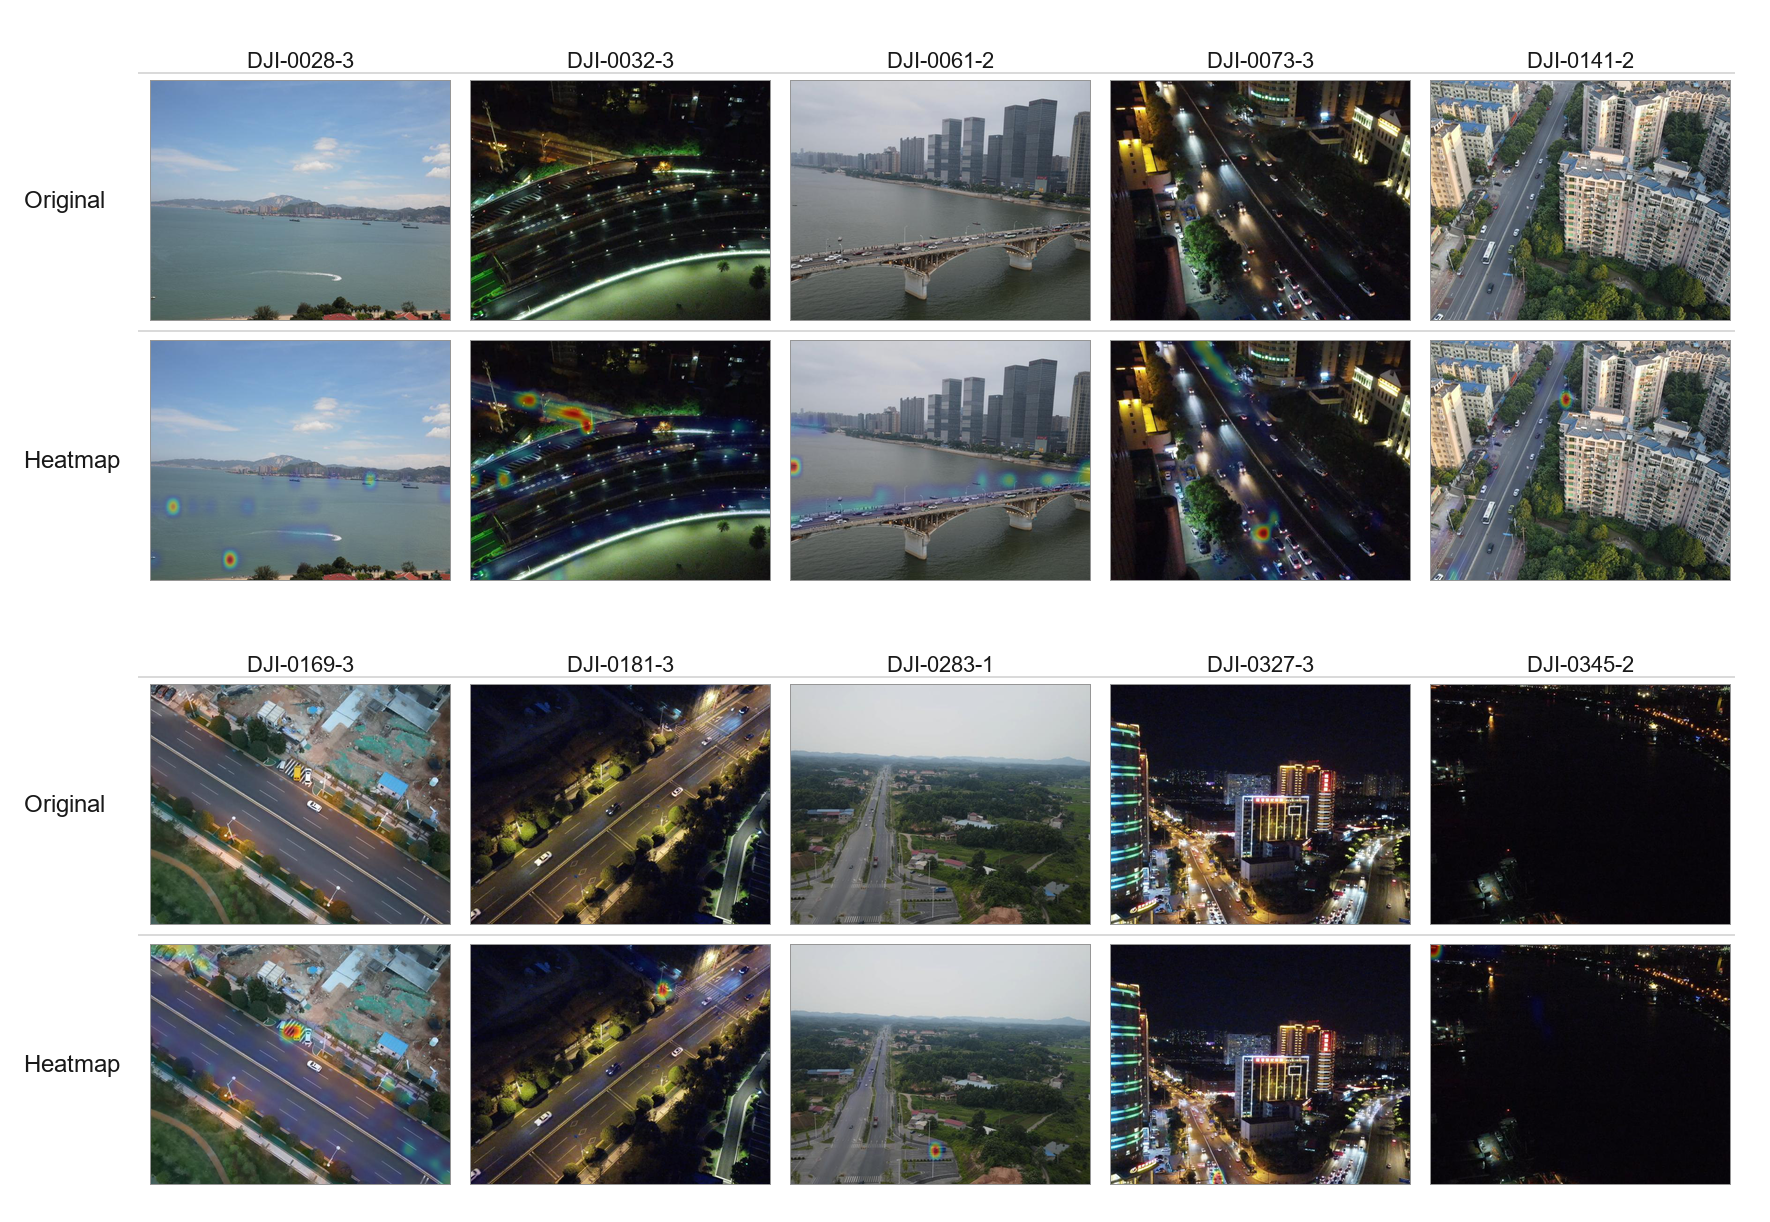
\includegraphics[width=0.88\linewidth]{images/chapter5/vt_tiny_mot_heatmap_overview.png}
  \caption{Original frames and anomaly heatmaps for the VT-Tiny-MOT test sequences. Each group contains five sequences. Within each group, the upper row shows the original frames, and the lower row shows the corresponding score-weighted heatmap visualization. The heatmaps visualize model-derived anomaly evidence rather than manually annotated abnormal regions.}
  \label{fig:chapter5-heatmap-examples}
\end{figure}

Across the ten test sequences, the heatmaps localize high-scoring trajectory evidence to specific scene regions when such evidence is spatially concentrated. Sequences with weaker or scattered scores produce diffuse low-intensity maps. These observations are consistent with the intended role of the heatmap as a scene-level visualization of object-aligned anomaly evidence.

\subsection{Discussion}
Because the current VT-Tiny-MOT output does not include manually verified anomaly labels, the experiment should be interpreted as a functional and qualitative demonstration rather than a quantitative detection benchmark. The experiment shows that fused trajectory-level anomaly evidence can be projected into spatial situation indicators, but it does not establish detection accuracy. A more complete evaluation would require frame-level or event-level anomaly annotations, which would make it possible to compare individual-only, group-only, and fused settings quantitatively.

\section{Chapter Summary}
This chapter developed a behavior anomaly detection framework based on the fused multimodal entities generated in Chapter 4. The task was defined as estimating individual and group anomaly evidence from fused trajectories, integrating them into object-level anomaly decisions, and projecting the results into regional situation indicators.

At the individual level, the method decomposes fused trajectories into route, speed, and shape representations. Masked LSTM autoencoders learn normal patterns, neighborhood-adjusted reconstruction errors produce branch-level scores, and rank-based ensemble scoring yields the final individual anomaly score.

At the group level, the chapter constructed a lightweight spatio-temporal graph in which target-frame nodes are linked by spatial group relations and temporal track continuity. Simple graph statistics describe interpretable events such as leaving, motion inconsistency, population change, split, and merge. Individual and group evidence are finally fused into anomaly-event scores and situation heatmaps. Under the qualitative evaluation setting used in this chapter, these outputs provide object-level anomaly cues and scene-level interpretation.

\chapter{System Implementation and Integrated Demonstration}

\section{Implementation Overview and Environment}
This chapter describes the implementation prototype of the multimodal target fusion and behavior analysis system. The purpose of this chapter is not to introduce a new algorithm, but to show how the system architecture defined in Chapter 2 and the methods developed in Chapters 3, 4, and 5 are organized into a runnable demonstration system.

The system environment is summarized in Table~\ref{tab:chapter6-env}. The implementation uses Python scripts for data processing, result adaptation, metric aggregation, and visualization payload generation. The demonstration interface is implemented as a static web page using HTML, CSS, and JavaScript. It can be opened locally in a browser or deployed as a static page for public demonstration. The experimental scripts are designed to use project-relative paths when transferring artifacts, so that the system is not bound to one fixed local directory.

\begin{table}[H]
  \centering
  \caption{Implementation environment of the demonstration system.}
  \label{tab:chapter6-env}
  \setlength{\tabcolsep}{4pt}
  \renewcommand{\arraystretch}{0.95}
  \small
  \begin{tabular}{p{0.24\linewidth}p{0.64\linewidth}}
    \toprule
    Component & Implementation description \\
    \midrule
    Offline processing & Python-based scripts for reading datasets, adapting experimental outputs, computing metrics, and generating visualization records. \\
    Data artifacts & Sequence metadata, trajectory records, anomaly labels or protocols, method scores, registration diagnostics, and frame-level visualization payloads. \\
    Demonstration interface & Static browser-based page implemented with HTML, CSS, and JavaScript. \\
    Deployment mode & Local browser preview and static-page deployment, such as GitHub Pages. \\
    Path organization & Relative project paths are used for generated artifacts to improve portability across local and remote environments. \\
    \bottomrule
  \end{tabular}
\end{table}

The implemented system follows the six functional layers introduced in Chapter 2: multimodal data input, preprocessing, optical reference retrieval, entity-level fusion, behavior analysis, and result presentation. In the prototype, algorithmic experiments and result generation are performed offline. The system then organizes the generated trajectories, anomaly scores, registration diagnostics, heatmaps, and explanation records into a unified visualization package. This design allows the experimental algorithms to be updated independently while keeping the presentation interface stable.

This environment summary defines the engineering boundary of the prototype. The following module description then explains how the implementation corresponds to the architectural layers introduced earlier.

\section{Open-source Repository and Reproducibility}
The implementation code, thesis source files, experimental scripts, and visualization materials of this project are organized in a public GitHub repository: \url{https://github.com/wcx12/FusionTrack}. The repository is used as the reproducibility entry for the implemented system. It provides the LaTeX source of the thesis, anomaly detection benchmark scripts, VPR and registration modules, static visualization materials, and workflow files for document building.

The open-source package is organized around the same modular boundary as the system implementation. The benchmark code defines data protocols, result adapters, metric computation, and key-audit rules. The visualization materials provide the static demonstration page and generated result files used for thesis presentation. The repository does not include large raw datasets, server credentials, private configuration files, or absolute local paths. This separation keeps the public materials inspectable while avoiding dependence on one local machine or remote server account.

\section{Implementation of Main Modules}
To keep the implementation consistent with the system model in Chapter 2, the prototype maps each architectural layer to a concrete system module. The data input and preprocessing modules form the entry of the system. They read the available dataset sequences and experimental results, then normalize them into records indexed by sequence, frame, target, method, and score. This organization follows the target-centered representation defined in Chapter 2 and makes later result comparison more direct.

The optical reference retrieval module corresponds to Chapter 3. In the system implementation, TF-VPR is treated as a reference retrieval component for coordinate-missing optical images. Its output is used as a scene-level constraint or as an experimental result interface, rather than as a direct target identity decision.

The entity-level fusion and registration module corresponds to Chapter 4. The implementation preserves the registration and fusion outputs in a form suitable for inspection, including correspondence-related records, fused trajectory information, and diagnostic indicators. These outputs support the later behavior analysis module.

The behavior analysis module corresponds to Chapter 5. It organizes individual anomaly results, group anomaly results, fused anomaly evidence, event explanations, and situation heatmaps. The module does not only output a scalar score; it also preserves the visual and textual evidence required for interpreting abnormal behavior.

The result presentation module finally converts these records into an interactive demonstration interface. It presents metrics, dynamic visualization, method comparison, explanation records, language switching, and report export, so that the outputs of the previous modules can be inspected in a unified page.

\section{System Workflow}
The runtime workflow of the implemented system is organized around experimental result loading and visualization generation. First, the system reads dataset metadata, frame resources, trajectory records, and method outputs. Second, the result adaptation module converts these files into a unified format. Third, the metric module summarizes sequence-level and method-level indicators. Fourth, the visualization module generates the dynamic payload used by the web interface, including original frames, trajectory overlays, heatmaps, and combined views. Finally, the static page loads these records and provides interactive inspection.

In compact form, the workflow consists of data and result loading, unified result adaptation, metric aggregation, visualization payload generation, and web-based demonstration with export.

This workflow separates algorithm execution from result presentation. Therefore, when a stronger detector, fusion method, or registration algorithm is added later, it only needs to provide outputs in the agreed result format. The visualization layer can then reuse the same interface to display the updated results.

\section{Integrated Demonstration Interface}
The integrated demonstration interface is designed to support thesis presentation and result inspection. The top part of the interface provides method selection, sequence selection, language switching, and core indicators. These controls allow the user to compare different methods and inspect the results of different sequences without changing the underlying data files.

The central visualization area provides four synchronized views: the original video, the anomaly heatmap, the trajectory view, and the combined heatmap-trajectory view. The original video keeps the scene context visible. The heatmap view shows where abnormal evidence is concentrated. The trajectory view highlights target movement patterns. The combined view is used as the default display because it presents spatial risk and target motion at the same time.

The system also separates different result types. Individual-level results focus on abnormal behavior of a single target, such as route deviation or motion irregularity. Group-level results focus on relational changes among multiple targets, such as leaving, merging, splitting, or neighborhood restructuring. Registration diagnostics are presented separately to avoid mixing cross-modal alignment quality with video anomaly detection results.

In addition to dynamic visualization, the interface provides explanation records, protocol information, data audit information, and result export. These functions make the system more suitable for thesis demonstration: the main page can remain concise during presentation, while detailed evidence can still be expanded when needed.

\section{Chapter Summary}
This chapter presented the implementation prototype and integrated demonstration of the proposed system. Different from Chapter 2, which defines the system architecture and data model, this chapter focuses on how the architecture is realized in an offline processing and web-based presentation workflow.

The implemented prototype connects the TF-VPR reference retrieval interface, entity-level fusion and registration outputs, individual and group anomaly analysis results, and situation heatmap visualization. Through unified result adaptation and static web presentation, the system provides a runnable demonstration for the methods developed in the previous chapters. The prototype also keeps the result interface modular, allowing later algorithmic improvements to be integrated without redesigning the whole visualization system.

\chapter{Conclusion and Future Work}

\section{Summary of the Thesis}
This thesis studied multimodal target trajectory completion, fusion, and behavior analysis under incomplete and heterogeneous observations. The core problem is that different sensing sources may observe the same physical target with different coordinate availability, sampling density, attribute form, and reliability. Directly combining such observations can easily produce unstable identities or noisy behavior results. To address this issue, the thesis built a progressive framework from optical reference retrieval to multimodal entity fusion and behavior analysis.

First, the thesis established a unified target-centered representation for heterogeneous observations. Optical, electromagnetic, SAR, thermal, and trajectory-based sources are organized with position, motion, attributes, confidence, and validity information. This representation provides the basis for subsequent module connection.

Second, for coordinate-missing optical images, the thesis adopted TF-VPR as the optical reference retrieval module. The module retrieves coordinate-known reference images instead of directly estimating geographic coordinates from a single query image. The retrieved Top-\(k\) references provide scene-level anchors for downstream target association, allowing coordinate-missing optical observations to enter the trajectory system.

Third, the thesis formulated multimodal target fusion as an entity-level registration problem. Completed trajectories from different modalities are encoded into entity embeddings, refined through multi-set graph matching, and merged through reliability-aware fusion. The result is a fused target representation that combines trajectory information, modality-specific attributes, and confidence information.

Finally, the fused entities were used for behavior analysis. Individual behavior is described through route, speed, and shape features, while group behavior is modeled through dynamic spatiotemporal relations. Individual and group evidence are then combined into anomaly scores, event decisions, and regional situation heatmaps.

Overall, the thesis provides a coherent technical route from incomplete multimodal observations to fused target representation and behavior-level interpretation. The main value of the work lies in connecting optical reference retrieval, entity-level fusion, and behavior analysis into one consistent framework.

\section{Limitations}
Several limitations remain. First, the optical completion stage still depends on the quality of both reference retrieval and downstream target association. TF-VPR provides scene-level candidate references, but target-level correspondence may remain uncertain under large viewpoint changes, occlusion, weak target appearance, or inaccurate detections.

Second, multimodal fusion and behavior analysis depend on the coverage and quality of upstream trajectories. When all modalities are severely incomplete or entity embeddings are weak, graph matching and reliability-aware fusion may still produce uncertain correspondences. In addition, group-level behavior evaluation is limited by the lack of complete anomaly annotations, so some results rely on ranking analysis and qualitative inspection.

Finally, the current system is still a research prototype. It verifies the feasibility of the overall pipeline, but real-time processing, large-scale data management, automatic parameter adaptation, and long-term deployment stability still require further work.

\section{Future Work}
Future work can proceed in three directions. First, optical trajectory completion can be strengthened by combining scene-level VPR retrieval with more explicit target-level matching. Object appearance, local geometry, temporal consistency, and detection confidence could be jointly used after Top-\(k\) retrieval.

Second, more complete multimodal datasets are needed. Such datasets should include cross-modal target identities, incomplete trajectory segments, coordinate-missing optical images, and behavior anomaly annotations. They would support more direct evaluation of optical completion, entity registration, fusion quality, and behavior analysis within the same benchmark.

Third, the framework can be improved for practical deployment. Future work should propagate calibrated uncertainty across modules, expand behavior analysis with richer semantic and group context, and optimize the system for efficient retrieval, incremental graph matching, streaming anomaly analysis, and stable long-sequence visualization.


% 后置内容
\backmatter

% 参考文献：
% 添加文献时，请按 BibTeX 格式添加至 misc/ref.bib，并在正文所需位置使用 \cite{…} 引用。
% 如无特殊需要，无需改动相应 TeX 文件。
\input{misc/2_references.tex}
% 附录：暂不使用，如需恢复可取消下一行注释
% \chapter{Additional Registration Benchmark Results}
\label{chap:appendix-registration-benchmark}

This appendix collects the extended registration results that are not required for the main argument of Chapter 4 but are useful for checking the behavior of the registration module across datasets. All tables use the same source-to-reference convention. Rotation error is reported in degrees, translation error is the Euclidean translation error, and Chamfer distance is computed after applying the predicted transformation. The scalar pose metric is
\begin{equation}
  \mathrm{Pose}= \mathrm{RRE} + 50 \times \mathrm{RTE}.
\end{equation}
Lower values indicate better performance. A missing Chamfer entry means that the corresponding official log did not provide point-level outputs needed for this metric.

\section{ModelNet40 Source-2/Crop Protocol}

Table~\ref{tab:appendix-modelnet40-registration} reports the ModelNet40 source-2/crop results. The learned rows use the completed full-set evaluation, while the non-learning rows use the protocol-aligned 20-batch validation subset. The two groups therefore should not be read as having identical sample counts, but they do share the same transformation direction and metric definitions. The latest long MPS-GAF convergence run is not included here because its final evaluation had not been completed when this appendix was prepared.

This protocol is kept in the appendix rather than the main chapter because it is mainly used as supporting evidence. The main body only needs the conclusion that MPS-GAF remains competitive on the intended object-level source-2/crop setting. The appendix gives the detailed rows so that the comparison with learning-based and non-learning baselines can be checked directly without interrupting the main argument.

When reading the table, the most relevant comparison is between MPS-GAF and RPM-Net because both are evaluated on the same completed learning-based split. The non-learning rows are retained as calibration baselines for local registration behavior, so their smaller pair count should be interpreted as a protocol note rather than as a direct full-set ranking.

\begin{table}[H]
  \centering
  \caption{ModelNet40 source-2/crop registration results.}
  \label{tab:appendix-modelnet40-registration}
  \scriptsize
  \begin{tabular}{llrrrrr}
    \toprule
    Method & Type & Pairs & Pose & RRE & RTE & Chamfer \\
    \midrule
    MPS-GAF & learning & 4936 & \textbf{15.875} & \textbf{9.982} & 0.118 & 0.033 \\
    RPM-Net & learning & 4936 & 16.242 & 10.428 & \textbf{0.116} & 0.036 \\
    DCP-DGCNN & learning & 4936 & 40.356 & 24.094 & 0.325 & 0.057 \\
    PointNetLK & learning & 4936 & 47.444 & 31.708 & 0.315 & 0.041 \\
    PRNet-DGCNN & learning & 4936 & 51.879 & 31.763 & 0.402 & 0.077 \\
    IDAM-GNN & learning & 4936 & 56.648 & 37.875 & 0.375 & 0.075 \\
    OMNet & learning & 4936 & 173.830 & 127.799 & 0.921 & 1.034 \\
    ICP point-to-point & non-learning & 160 & 34.662 & 22.619 & 0.241 & 0.024 \\
    ICP point-to-plane & non-learning & 160 & 36.604 & 25.401 & 0.224 & 0.059 \\
    CPD rigid & non-learning & 160 & 38.109 & 25.328 & 0.256 & \textbf{0.021} \\
    Trimmed ICP & non-learning & 160 & 38.148 & 24.658 & 0.270 & 0.041 \\
    SC2-PCR-FPFH & non-learning & 160 & 90.881 & 71.574 & 0.386 & 0.038 \\
    MAC-FPFH & non-learning & 160 & 103.229 & 81.698 & 0.431 & 0.049 \\
    KISS-Matcher & non-learning & 160 & 114.931 & 86.175 & 0.575 & 0.170 \\
    \bottomrule
  \end{tabular}
\end{table}

The ModelNet40 result is the clearest completed evidence for the proposed method. MPS-GAF and RPM-Net have similar translation error, but MPS-GAF gives the lower pose metric because its rotation error is smaller. The ICP and CPD rows remain useful local-registration references, especially for Chamfer distance, but their pose errors are higher under the two-source crop setting. The recent robust estimators based on FPFH correspondences are weaker in this object-level protocol, which suggests that the correspondence stage is the limiting factor for those rows.

\section{3DMatch}

Table~\ref{tab:appendix-3dmatch-registration} reports the 3DMatch results. This benchmark uses indoor fragment pairs rather than object-level ModelNet shapes. The stronger rows are therefore the methods designed for this benchmark family, especially GeoTransformer-style models. The MPS-GAF rows are included as adapter-based generalization checks.

This table is mainly used to show the cross-domain behavior of the registration module. It separates object-level performance from indoor-fragment performance and prevents the main chapter from overclaiming a single method as universally strongest across all registration protocols.

\begin{table}[H]
  \centering
  \caption{3DMatch registration results.}
  \label{tab:appendix-3dmatch-registration}
  \scriptsize
  \resizebox{\textwidth}{!}{%
  \begin{tabular}{llrrrrr}
    \toprule
    Method & Type & Pairs & Pose & RRE & RTE & Chamfer \\
    \midrule
    PointRegGPT GeoTransformer-16w & learning & 1623 & \textbf{12.701} & 5.387 & 0.146 & 0.383 \\
    RoITr & learning & 1623 & 12.850 & \textbf{5.038} & 0.156 & n/a \\
    PointRegGPT GeoTransformer-2w & learning & 1623 & 13.413 & 5.636 & 0.156 & 0.378 \\
    GeoTransformer & learning & 1623 & 14.310 & 6.010 & 0.166 & 0.382 \\
    RPM-Net & learning & 1623 & 75.478 & 31.375 & 0.882 & 0.171 \\
    MPS-GAF no-normals & learning & 1623 & 87.580 & 35.224 & 1.047 & 0.238 \\
    ICP point-to-point & non-learning & 1623 & 90.941 & 37.234 & 1.074 & \textbf{0.157} \\
    KISS-Matcher & non-learning & 1623 & 143.361 & 58.484 & 1.698 & 0.644 \\
    SC2-PCR-FPFH & non-learning & 1623 & 171.613 & 75.110 & 1.930 & 0.242 \\
    MAC-FPFH & non-learning & 1623 & 193.811 & 85.778 & 2.161 & 0.314 \\
    TurboReg & non-learning & 1623 & 204.595 & 87.252 & 2.347 & 0.605 \\
    TEASER++ & non-learning & 1623 & 236.522 & 99.907 & 2.732 & 0.648 \\
    \bottomrule
  \end{tabular}}
\end{table}

The 3DMatch table shows a clear domain effect. GeoTransformer, PointRegGPT, and RoITr are much stronger than the ModelNet-oriented learned baselines and the FPFH-driven robust estimators. MPS-GAF is close to simple ICP in pose but does not reach the indoor-fragment methods. This is not a contradiction with the ModelNet40 result; it reflects a change in data distribution, overlap pattern, and descriptor requirement.

\section{3DLoMatch}

Table~\ref{tab:appendix-3dlomatch-registration} reports the low-overlap 3DLoMatch results. This split is more difficult than 3DMatch because the valid common region between fragments is smaller. The same pattern appears, but the gap between specialized indoor-fragment methods and general adapters becomes larger.

The low-overlap setting is included because it is a useful stress test for correspondence quality. If a method relies too heavily on dense overlap or stable local neighborhoods, the degradation on this split becomes visible in both rotation and translation errors.

\begin{table}[H]
  \centering
  \caption{3DLoMatch registration results.}
  \label{tab:appendix-3dlomatch-registration}
  \scriptsize
  \resizebox{\textwidth}{!}{%
  \begin{tabular}{llrrrrr}
    \toprule
    Method & Type & Pairs & Pose & RRE & RTE & Chamfer \\
    \midrule
    PointRegGPT GeoTransformer-16w & learning & 1781 & \textbf{43.915} & \textbf{19.109} & \textbf{0.496} & 1.198 \\
    RoITr & learning & 1781 & 49.261 & 22.016 & 0.545 & n/a \\
    PointRegGPT GeoTransformer-2w & learning & 1781 & 49.570 & 22.182 & 0.548 & 1.199 \\
    GeoTransformer & learning & 1781 & 52.085 & 23.064 & 0.580 & 1.173 \\
    DCP-DGCNN & learning & 1781 & 132.011 & 58.091 & 1.478 & 0.344 \\
    RPM-Net & learning & 1781 & 139.609 & 61.549 & 1.561 & \textbf{0.260} \\
    MPS-GAF no-normals & learning & 1781 & 159.735 & 68.663 & 1.821 & 0.390 \\
    ICP point-to-point & non-learning & 1781 & 163.244 & 70.714 & 1.851 & 0.324 \\
    KISS-Matcher & non-learning & 1781 & 245.428 & 109.374 & 2.721 & 1.182 \\
    SC2-PCR-FPFH & non-learning & 1781 & 255.500 & 118.516 & 2.740 & 0.370 \\
    MAC-FPFH & non-learning & 1781 & 259.660 & 119.976 & 2.794 & 0.475 \\
    TurboReg & non-learning & 1781 & 264.655 & 118.473 & 2.924 & 0.854 \\
    TEASER++ & non-learning & 1781 & 273.181 & 120.558 & 3.052 & 0.844 \\
    \bottomrule
  \end{tabular}}
\end{table}

The MPS-GAF row remains slightly better than point-to-point ICP in pose, but it is far behind the 3DMatch-family networks. Low overlap makes the correspondence problem more dependent on benchmark-specific descriptors and robust correspondence filtering. The result is still useful because it marks the current boundary of the method: the multi-source mechanism helps in the controlled object setting, but it does not by itself solve low-overlap indoor fragment registration.

\section{ETH Laser Benchmark}

Table~\ref{tab:appendix-eth-registration} reports the ETH laser benchmark results. These rows should be read as cross-dataset generalization tests. The learned models were not trained specifically on ETH, and the point sampling differs from the indoor-fragment setting.

The ETH rows are therefore not used to replace the main ModelNet40 conclusion. They are included to clarify the current boundary of the implementation and to show that classical local registration can still be stronger when the scan statistics differ substantially from the learning-based training domain.

\begin{table}[H]
  \centering
  \caption{ETH laser benchmark registration results.}
  \label{tab:appendix-eth-registration}
  \scriptsize
  \resizebox{\textwidth}{!}{%
  \begin{tabular}{llrrrrr}
    \toprule
    Method & Type & Pairs & Pose & RRE & RTE & Chamfer \\
    \midrule
    ICP point-to-point & non-learning & 713 & \textbf{130.479} & 56.305 & \textbf{1.483} & \textbf{2.491} \\
    ICP point-to-plane & non-learning & 713 & 139.088 & 55.665 & 1.668 & 2.960 \\
    RANSAC-ICP & non-learning & 713 & 140.915 & 58.550 & 1.647 & 2.669 \\
    Trimmed ICP & non-learning & 713 & 144.889 & 57.732 & 1.743 & 2.933 \\
    Identity / FPFH-RANSAC 5k & non-learning & 713 & 147.959 & 59.179 & 1.776 & 3.113 \\
    MPS-GAF PPF & learning & 713 & 154.034 & 58.881 & 1.903 & 2.936 \\
    RPM-Net & learning & 713 & 154.968 & 57.363 & 1.952 & 2.716 \\
    MPS-GAF no-normals & learning & 713 & 176.900 & 57.272 & 2.393 & 3.115 \\
    TurboReg & non-learning & 713 & 237.778 & 107.603 & 2.603 & 11.737 \\
    GeoTransformer & learning & 713 & 287.792 & 119.915 & 3.358 & 17.397 \\
    PointRegGPT GeoTransformer-16w & learning & 713 & 345.705 & 97.922 & 4.956 & 23.101 \\
    TEASER++ & non-learning & 713 & 400.827 & 121.112 & 5.594 & 14.453 \\
    \bottomrule
  \end{tabular}}
\end{table}

ETH gives a different conclusion from ModelNet40. The completed rows are led by ICP variants, while the learned rows are weaker. The most likely reason is not a single implementation error: the same source-to-reference metric convention was used, and the inverse-transform diagnostic did not improve the learned rows. The result is better understood as a cross-domain limitation. ETH laser scans have different density, scale, and surface statistics from the object-level ModelNet40 setting and from the 3DMatch indoor fragments.

Overall, the appendix supports a narrower claim than a single aggregate table would suggest. MPS-GAF is strong on the intended ModelNet40 source-2/crop protocol and has completed checks on 3DMatch, 3DLoMatch, and ETH. On indoor fragment benchmarks, methods trained around the 3DMatch family remain stronger. On ETH, classical local registration is still the most reliable among the completed rows. These results clarify where the current method is effective and where dataset-specific adaptation is still needed.

\chapter{Source Code and Reproducibility Materials}
\label{chap:appendix-source-code}

The source code and related reproducibility materials of this thesis are publicly available at \url{https://github.com/wcx12/FusionTrack}. This appendix summarizes the role of the repository so that the relationship between the written thesis, experimental code, and demonstration system can be inspected directly.

The repository contains five main types of materials. The \texttt{article\_content/} directory stores the LaTeX source files, figures, references, and build configuration of the thesis. The \texttt{code/anomaly\_detection/benchmark/} directory stores the benchmark implementation for individual and group anomaly analysis, including protocol definitions, method adapters, metric computation, and result checking scripts. The \texttt{code/vpr/} directory stores the visual place recognition related implementation used by the coordinate-missing optical access module. The \texttt{code/registration/} directory stores the registration and fusion related code used by the entity-level fusion experiments. The \texttt{visualization\_results/} directory stores the static web demonstration and generated visualization materials used in the system presentation.

The open-source package is intended to support three forms of inspection. First, the thesis source can be rebuilt to check whether the written report, figures, tables, and references are consistent. Second, the benchmark scripts can be used to inspect the evaluation protocol and reproduce or extend the anomaly detection experiments after the required data are prepared. Third, the visualization materials provide a browser-based demonstration entry for checking the integrated output of the system, including sequence-level results, trajectory overlays, heatmaps, and explanation records.

Some materials are intentionally excluded from the public repository. Large raw datasets, server-side temporary artifacts, private credentials, local absolute paths, and machine-specific configuration files are not version controlled. These files are either too large, environment-dependent, or unsuitable for public release. The public repository therefore focuses on source code, reproducibility scripts, thesis source files, and shareable visualization artifacts.

% 致谢：在相应 TeX 文件撰写
%%
% BIThesis 本科毕业设计论文模板（全英文） —— 使用 XeLaTeX 编译 The BIThesis Template for Undergraduate Thesis
% This file has no copyright assigned and is placed in the Public Domain.
%%

\begin{acknowledgements}
The completion of this thesis would not have been possible without the guidance, help, and support of many people. First, I would like to express my sincere gratitude to my university supervisor, Prof. Jinhui Pang, for her guidance throughout my graduation project. From the selection of the research topic and the clarification of the research ideas to the adjustment of the thesis structure and the revision of the manuscript, Prof. Pang provided patient support and valuable suggestions. Her guidance helped me gradually identify the focus of the work and complete the thesis.

I am also grateful to my external supervisor, Mr. Haitao Zhang, for her guidance and support in the practical and engineering aspects of this project. Her advice helped me gain a clearer understanding of the application background of multimodal target fusion and behavior analysis systems. During the research and implementation process, Zhuoyi Yang also provided direct and detailed assistance in technical discussions, experimental progress, and thesis improvement. I would like to express my sincere thanks to him as well.

In addition, I would like to thank all the teachers in the School for their instruction during my undergraduate study. Their teaching helped me build the professional foundation and engineering ability required for this project. I also thank my classmates and friends for their help in literature search, technical discussion, and thesis revision. Finally, I am deeply grateful to my family for their constant understanding and support in my study and daily life. Due to my limited ability and experience, this thesis may still contain shortcomings, and I sincerely welcome criticism and corrections from the teachers.
\end{acknowledgements}


\end{document}
